\input{preamble}
\title{More than One Way to Skin a Cat:\\
Preserving Verified Modes in RLVR}
\author{Anonymous Authors}
\begin{document}
\maketitle

\begin{abstract}
A mathematical reasoning model can become more accurate while losing alternative
correct solutions. To measure this loss, we introduce \mb{}, a benchmark of
five executable domains that identifies different correct outputs for one problem. We then show that ReplayMaxRL, which combines sampling-aware
reinforcement learning with a memory of previously verified outputs, improves
correctness while preserving more valid alternatives. We find gains from replay
with both GRPO and MaxRL, across three and two model scales respectively,
and on a harder graph-coloring task. These results separate two requirements
often treated as one: discovering successful behaviors and preserving them.
\end{abstract}

\section{Correct answers can conceal the loss of alternatives}
\label{sec:introduction}\label{sec:collapse}
Reinforcement learning with verifiable rewards (RLVR) trains from executable
correctness feedback \citep{guo2025deepseekr1}, rewarding
familiar and new correct solutions alike. In mathematical search, losing
alternatives narrows the verified candidate set available from repeated sampling
\citep{brown2024monkeys,snell2024testtime}. Figure~\ref{fig:story} shows this
failure: correctness rises while sampled alternatives disappear.

\begin{figure}[!htbp]
\centering
\includegraphics[width=\linewidth]{figures/modecollapse_story.pdf}
\caption{\textbf{Correctness can rise while alternatives disappear.}
One graph admits six valid colorings. Bars pool four eight-sample draws from
matched Qwen2.5-3B runs. At pass 6.5, Dr.GRPO produces 22/32 correct from one
mode; ReplayMaxRL produces 32/32 across four.}
\label{fig:story}
\end{figure}

The loss also appears across our datasets. Averaged over five domains, eight
passes of Dr.GRPO reduce the initial number of verified alternatives beyond
the first correct output in eight samples by $99.4\%$ at Qwen2.5-0.5B,
$71.6\%$ at Falcon3-1B, and $41.5\%$ at Qwen2.5-3B
(Appendix Figure~\ref{fig:baseline-precheck}).

In an idealized model, our analysis shows that additional parameters can
preserve more sampled alternatives at matched accuracy when they strengthen
updates shared across correct outputs
(Appendix~\ref{app:theory-size}, Theorem~\ref{thm:shared-correctness});
size alone provides no guarantee.
We therefore ask how training can retain alternatives after they become rare.

\section{ModeBench makes output identity executable}
\label{sec:modebench}
To distinguish a different solution from a different string, \mb{} assigns each
accepted output a canonical key; each distinct key defines a verified
\emph{mode}. The validator returns both correctness and identity
(Figure~\ref{fig:modebench-examples}): computation routes in
Countdown and MathIR, tested program behaviors in Python, and valid
configurations in Graph and PantryPlan. Cosmetic aliases merge; distinct routes can share an answer
(key rules: Appendix~\ref{app:domain-overview}).

\begin{figure}[!htbp]
\centering
\includegraphics[trim={0 9bp 0 0},clip,width=\linewidth]{figures/modebench_examples.pdf}
\caption{\textbf{One prompt, different verified outputs.}
Keys retain a color vector, normalized computation tree, tested return vector,
algebraic state trajectory, or ingredient support. Cosmetic aliases merge;
these keys identify task-defined outputs rather than free-form reasoning.}
\label{fig:modebench-examples}
\end{figure}

\section{ReplayMaxRL: learn from new samples and remember successes}
\label{sec:method}\label{sec:maxrl-method}\label{sec:replay}
Output identity also makes preservation actionable. A verified mode missing
from fresh rollouts supplies no direct on-policy signal. ReplayMaxRL pairs fresh learning with a memory of earlier successes
(Figure~\ref{fig:verified-support-story}).

\begin{figure}[!htbp]
\centering
% Crop only blank PDF margins; keep the figure itself unchanged.
\includegraphics[trim={4bp 23bp 4bp 10bp},clip,width=\linewidth]{figures/verified_support_story.pdf}
\caption{\textbf{Discovery and preservation use the same verified samples.}
MaxRL learns from fresh rewards; replay retains exemplars by key and revisits
rare successes. Memory cannot protect a mode before it is discovered.}
\label{fig:verified-support-story}
\end{figure}

MaxRL trains policy $\pi_\theta$ for success within $k$ samples across sampling
budgets \citep{tajwar2026maxrl}. Each training prompt $x$ keeps one
policy-generated exemplar $e_c$ per admitted key in bank $\mathcal B_x$.
With $|e_c|$ its token length, recurrent replay minimizes
\begin{equation}
L_{\mathrm{replay}}(x)=-\frac{1}{|\mathcal B_x|}
\sum_{c\in\mathcal B_x}\frac{\log\pi_\theta(e_c\mid x)}{|e_c|}.
\label{eq:lm-verified-replay}
\end{equation}
Equal averaging of per-token scores makes replay independent of discovery frequency. Replacing MaxRL with Dr.GRPO \citep{liu2025understanding},
which debiases GRPO \citep{shao2024deepseekmath}, yields our ReplayDr.GRPO.
Appendix~\ref{app:algorithm} gives
the full update. Appendix~\ref{app:theory} proves categorical collapse and
replay retention (Theorems~\ref{thm:grpo-collapse} and~\ref{thm:replay-retention}).

\noindent\textbf{Related work.} Prior work studies diversity collapse
\citep{cui2025entropy,dang2025diversity}, sampling-aware objectives, and success
replay \citep{zhang2025rlep}. Our focus is execution-defined identity for
measuring and retaining verified alternatives. Appendix~\ref{sec:related}
gives the full discussion.

\section{Does memory preserve useful output support?}
\label{sec:experiments}\label{sec:results}
We test whether remembering training successes benefits new problems.
\texttt{pass@8} is the chance that eight samples contain any correct response;
\texttt{distinct@8} is their average number of distinct verified modes. Reporting
both separates success from the alternatives available for selection, although
mode counts remain coupled to correctness (definitions: Appendix~\ref{app:metrics}).

Five seeds are registered per comparison for eight passes; each of 128 held-out prompts per
domain receives four eight-sample draws. Controls execute the replay code with its gradient zeroed. Figure~\ref{fig:cross-scale-terminal-effects} compares
Dr.GRPO with replay and alternatives targeting reward normalization, on-policy
diversity (UCPO; \citealp{lochab2026ucpo}), success replay (RLEP-Dr),
and semantic entropy. Protocols and uncertainty are in
Appendices~\ref{app:experimental-design} and~\ref{app:extended-results}.

\begin{figure}[!htbp]
\centering
\includegraphics[width=\linewidth]{figures/experiment1_retention_comparator_matrix.pdf}
\caption{\textbf{Replay improves correctness and verified support across scales.}
(A) ReplayDr.GRPO minus Dr.GRPO. (B) Qwen2.5-0.5B alternatives and the untrained
reference minus Dr.GRPO. Daggers mark four admissible pairs; others use five. Average uses shared seeds.
Left: probability differences. Right: key counts. Bold marks column maxima;
uncertainty: Appendix~\ref{app:supporting}.}
\label{fig:cross-scale-terminal-effects}
\end{figure}

\noindent\textbf{Memory improves the candidates available at evaluation.}
\label{sec:results-retention}
ReplayDr.GRPO improves both means in all 14 complete blocks and the remaining
four-seed block; \texttt{distinct@8} rises in all 74 admissible pairs
(source exclusion: Appendix~\ref{app:source-integrity}). On Qwen2.5-0.5B Countdown,
\texttt{pass@8} rises from $.48$ to $.67$ and \texttt{distinct@8} from $.49$
to $1.64$. The gain includes more computation routes alongside greater success.
These held-out prompts never enter the bank: replay improves candidates for new problems.
A matched weighting ablation favors uniform over fresh-frequency replay on
Graph, Countdown, and PantryPlan; Python and MathIR remain inconclusive
(Appendix~\ref{app:frequency-replay-progress}).

\clearpage
\begin{figure}[!htbp]
\centering
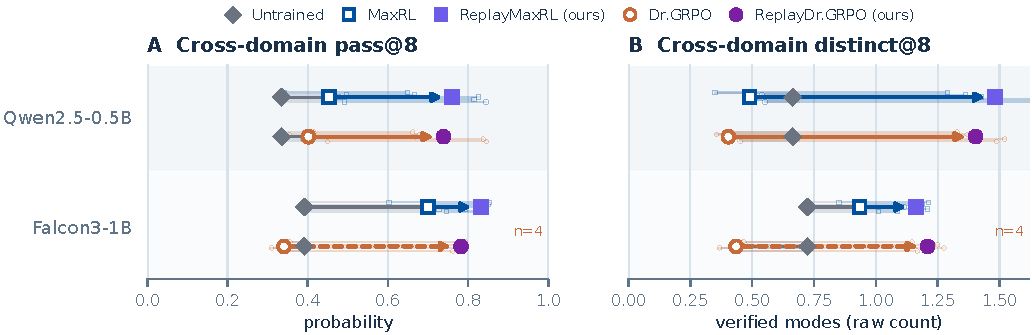
\includegraphics[width=\linewidth]{figures/e118_all_scale_factorial_progress.pdf}
\caption{\textbf{Memory adds value beyond sampling-aware MaxRL.}
Each track connects the untrained model, fresh-objective training, and its replay
counterpart. Faint paths are seeds; bold paths average domains within seed.
Falcon Dr.GRPO uses four common admissible seeds; other tracks use five. Both
means improve at both scales.}
\label{fig:maxrl-factorial}
\end{figure}

\noindent\textbf{Stronger fresh learning still benefits from memory.}
\label{sec:results-maxrl}
The first result leaves open whether a stronger fresh objective would suffice.
We therefore cross Dr.GRPO/MaxRL with replay absent/present
(Figure~\ref{fig:maxrl-factorial}). Replay improves both cross-domain averages
under both objectives; the Falcon Dr.GRPO track is descriptive at four seeds. For ReplayMaxRL, both
endpoints improve in all five Qwen domains; Falcon correctness improves in five
and breadth in four. The cross-domain averages are post-hoc summaries; paired intervals
are in Appendix~\ref{app:results-maxrl}. Improving success across sampling
budgets does not remove the value of revisiting earlier successes: fresh
learning still benefits from persistent memory.

\begin{figure}[!htbp]
\centering
\includegraphics[width=\linewidth]{figures/modebench_level_admission.pdf}
\caption{\textbf{Preservation matters on harder Graph.}
(A) Frozen-model success across levels. (B) Completed Level-2 Graph factorial:
small marks are five seeds, large marks their means. Every replay seed exceeds
every non-replay seed on both endpoints.}
\label{fig:level2-admission}
\end{figure}

\noindent\textbf{On harder problems, memory also changes the chance of success.}
\label{sec:results-levels}
We next test Level 2, which increases difficulty while preserving the validator,
key rule, and valid-mode-count histogram (Appendix~\ref{app:data}). On harder Graph,
Dr.GRPO/MaxRL reach $.20/.43$ \texttt{pass@8}, versus $.76/.74$ with replay.
The benefit extends to finding any correct candidate, giving memory a direct
performance stake (Figure~\ref{fig:level2-admission}). This complete
five-seed result covers Graph; other Level-2 domains remain incomplete.

\section{Conclusion and Limits}
\label{sec:conclusion}\label{sec:discussion}\label{sec:limitations}
Remembering earlier successes complements fresh learning: replay improves
held-out correctness and sampled output support. Evaluation should therefore
ask which verified alternatives remain available, alongside what training
learns to solve. These are small synthetic tasks, and replay can revisit only
discovered, retained modes. Individual mode survival
(Appendix~\ref{app:ablations}) and size-dependent update geometry remain
unmeasured. The results do not establish that broader support causes accuracy
gains, or that verified modes have downstream utility. Open-ended mathematical
reasoning remains an important test.

\label{main:lastpage}
\clearpage
\bibliographystyle{plainnat}
\bibliography{example_paper}
\clearpage
\appendix
% Supplementary material for the anonymous MATH-AI NeurIPS 2026 submission.
% The root document supplies \appendix, bibliography, packages, and macros.
% All original supplementary figures, tables, and labels are preserved.

\section*{Supplementary Material}
\label{app:organization}

The supplement expands the four-page paper in reading order.
Appendix~\ref{app:metrics} defines the measurements and explains the replay
objective. Appendix~\ref{app:experimental-design} gives the domain and
comparison designs; Appendix~\ref{app:extended-results} preserves the detailed
results behind the main figures. Related work appears in
Appendix~\ref{sec:related}, followed by the formal analysis in
Appendix~\ref{app:theory} and supporting comparisons in
Appendix~\ref{app:supporting}. The remaining sections specify the semantic
baseline, execution contracts, prompts, datasets, algorithm, mechanism checks,
scale extensions, and reproducibility record. Appendix~\ref{app:limitations}
states the limits and disclosures.


\long\def\directcomparatormaterial{%
\begin{table}[H]
  \centering
  \caption{\textbf{Direct alternatives to canonical mode-balanced replay.}
  Each method inherits the same eight-pass evaluation contract. Coverage counts
  source-admissible terminal runs; incomplete or excluded sources do not enter
  complete-block inference (Appendix~\ref{app:source-integrity}).}
  \label{tab:direct-comparators}
  \scriptsize
  \setlength{\tabcolsep}{3pt}
  \begin{tabularx}{\linewidth}{@{}P{.17\linewidth}P{.38\linewidth}YP{.12\linewidth}@{}}
    \toprule
    \textbf{Method} & \textbf{Active distinction} & \textbf{Question isolated}
      & \textbf{Coverage} \\
    \midrule
    Dr.GRPO & Group-centered binary reward; no auxiliary derivative &
      verifier-only reference & 75/75 \\
    GRPO & Reward-standardized group-relative update &
      estimator normalization & 75/75 \\
    ReplayDr.GRPO & One retained exemplar per verified key, sampled uniformly
      over keys & persistent canonical memory & 74/75 admissible \\
    UCPO & Reallocates positive advantage within the current rollout group &
      on-policy diversity incentive without memory & 50/75 \\
    Sparse RLEP-Dr & Replays verified successes in observed frequency, without
      canonical balancing & success memory without key balancing & 47/75 \\
    MaxRL & Optimizes best@\(k\) jointly across sampling budgets, without replay
      & sampling-aware fresh search without persistent memory & 11/15 blocks \\
    Fixed semantic entropy & Adds detached surprisal over verified canonical
      outcomes to Dr.GRPO & explicit within-rollout diversity incentive &
      10/15 blocks \\
    \bottomrule
  \end{tabularx}
\end{table}
}

\long\def\crossscaletablematerial{%

\begin{table}[H]
  \centering
  \caption{\textbf{Matched results after eight training passes.} Columns compare Dr.GRPO with ReplayDr.GRPO after exactly eight training passes. Entries are means over the displayed paired-seed intersection;
  $n$@pass gives its size and training pass. P, M, and D denote
  \texttt{pass@8}, \texttt{mean@8}, and \texttt{distinct@8}. Every available
  source-admissible terminal pair is included, no shallower checkpoint is carried forward, and
  no missing result is imputed. Falcon Countdown uses four admissible seeds
  (Appendix~\ref{app:source-integrity}). Pale green marks a ReplayDr.GRPO mean that is
  strictly higher than its matched Dr.GRPO mean.}
  \label{tab:core-terminal-endpoints}
  \scriptsize
  \setlength{\tabcolsep}{3.2pt}
  \resizebox{\linewidth}{!}{%
  \begin{tabular}{@{}llc*{6}{r}@{}}
    \toprule
    \textbf{Model} & \textbf{Domain} & \textbf{$n$@pass} &
      \multicolumn{3}{c}{\textbf{Dr.GRPO}} &
      \multicolumn{3}{c}{\textbf{ReplayDr.GRPO}} \\
    \cmidrule(lr){4-6}\cmidrule(l){7-9}
      & & & \textbf{P} & \textbf{M} & \textbf{D}
      & \textbf{P} & \textbf{M} & \textbf{D} \\
    \midrule
    \input{results/core_terminal_endpoints_table_body.tex}
  \end{tabular}}
\end{table}

}

\section{Extended Definitions and Objective Rationale}
\label{app:metrics}

Correctness and solution support are distinct properties of a policy. For a
prompt $x$ with reference specification $s_x$, the validator maps a response
to either failure or a canonical key:
\[
  V(\cdot,s_x):\mathcal Y\rightarrow \mathcal C_x\cup\{\bot\}.
\]
Here $\mathcal C_x$ is the set of valid solution keys and $\bot$ denotes
failure. The learner observes a key only for a response it generates; neither
the full set $\mathcal C_x$ nor its size is revealed.

For $Y\sim\pi_\theta(\cdot\mid x)$, the policy induces both a total probability
of verified success and a distribution over how that probability is allocated:
\[
 P_\theta^+(x)=\Pr[V(Y,s_x)\neq\bot],
 \qquad
 p_\theta^+(c\mid x)=\Pr[V(Y,s_x)=c\mid V(Y,s_x)\neq\bot].
\]
The conditional distribution is defined only when $P_\theta^+(x)>0$;
when $P_\theta^+(x)=0$, all three sampling metrics below are zero.
The first quantity measures correctness. The second describes the repertoire
of verified behaviors conditional on being correct. We call concentration of
$p_\theta^+$ onto fewer keys \emph{mode collapse}, particularly when
$P_\theta^+$ remains stable or increases.

\subsection{Measuring success and support}
\label{sec:collapse-metrics}

For $K$ independent samples $Y_{1:K}$, let
\[
  D_K=\bigl|\{V(Y_i,s_x):i\le K\}\setminus\{\bot\}\bigr|,
  \qquad
  F_K=K^{-1}\sum_i \1[V(Y_i,s_x)\neq\bot].
\]
ModeBench reports three averages with different units. \texttt{distinct@}$K
=\E[D_K]$ is an expected count in $[0,K]$ of unique verified keys;
\texttt{pass@}$K=\Pr[D_K>0]$ and \texttt{mean@}$K=\E[F_K]$ are probabilities
in $[0,1]$. For every draw, $F_K\le\1[D_K>0]\le D_K$; hence
$\texttt{mean@}K\le\texttt{pass@}K\le\texttt{distinct@}K$. The inequality is
valid, but equal numerical changes are not commensurate: $.02$ in
\texttt{pass@8} is two probability points, whereas $.02$ in
\texttt{distinct@8} is $.02$ expected verified keys.

For a fixed prompt, write $\mu_c(x)=\Pr[V(Y,s_x)=c]$. Independence gives
\[
 \texttt{pass@}K(x)=1-(1-P_\theta^+(x))^K,\qquad
 \texttt{distinct@}K(x)=\sum_{c\in\mathcal C_x}[1-(1-\mu_c(x))^K].
\]
These identities apply before averaging over prompts; applying the nonlinear
formula to an average success probability generally gives a different result.

Raw \texttt{distinct@}$K$ measures sampled coverage, not the total number of
positive-probability modes. For an uninformed reference, suppose a finite
space has $N$ actions and $n_c$ actions map to valid key $c$. Uniform independent
action sampling then gives $\sum_c[1-(1-n_c/N)^K]$ expected verified keys.
The simpler expression $m_x[1-(1-1/N)^K]$ applies when the $m_x$ valid actions
have distinct keys, as in our reported finite-action references.
Open-ended program and derivation spaces have no canonical nominal
``uniform'' generator.

The registered terminal co-primary endpoints are \texttt{pass@}$K$, the
probability of finding any correct output, and raw \texttt{distinct@}$K$, the
number of verified keys found. We report both separately for each
model--domain--level block. The derived contrast
$\texttt{distinct@}K-\texttt{pass@}K
=\E[D_K-\1[D_K>0]]$ is an interpretive decomposition: it estimates the
number of verified modes beyond the first. It is computable without knowing the
full valid set $\mathcal C_x$ and remains coupled to the number of successful
draws. We use it as an interpretive decomposition rather than a fully
success-matched diversity measure or a third primary endpoint. Because every
headline evaluation fixes $K=8$, reporting $\texttt{distinct@8}/8$ would add no
information beyond a linear rescaling; we retain the raw count and label its
units explicitly.

\subsection{Why binary rewards amplify common modes}
\label{sec:collapse-mechanism}

A binary reward identifies success but is indifferent among successful keys.
GRPO and Dr.GRPO center that reward within each sampled group, assigning every
correct response the same task credit regardless of its execution key. Key
frequency is therefore the remaining asymmetry: a common correct mode appears
in more updates, while an absent mode supplies no direct sampled signal.

A categorical reduction makes this feedback loop explicit. Let $p_c$ denote
the probability of correct mode $c$ and
$P=\sum_{c\in\mathcal C}p_c$ the total correct mass. Under Euclidean gradient
ascent in independently trained softmax logits on expected binary reward,
two correct modes $c$ and $d$ satisfy
\[
  \frac{d}{dt}\log\frac{p_c}{p_d}=(p_c-p_d)(1-P).
\]
Whenever incorrect mass remains, $p_c>p_d$ causes the log-odds gap to grow:
binary reward magnifies an existing imbalance rather than correcting it.
Finite on-policy groups add two sampling effects. An unsampled mode supplies
no direct sampled score term, while an all-correct group has zero centered
task advantage. The
full derivation and the GRPO/Dr.GRPO equivalence appear in
Appendix~\ref{app:theory}, which states the assumptions and distinguishes
this idealized mechanism from finite language-model training.



\subsection{Why key-balanced replay targets both success and support}
\label{app:replay-objective}

For a prompt $x$, the bank $\mathcal B_x$ contains one verified exemplar per
discovered key. The replay term applies equal weight to those keys.
Uniform sampling over keys prevents discovery frequency from determining replay
frequency. To explain its relationship to the evaluation metric, we first
analyze an equal-weight categorical surrogate, without length normalization.
A stored response's probability need not equal its key's total probability.
For $C=|\mathcal B_x|$ banked keys, write $p(c)$ for their probabilities
and $q_{\mathcal B}$ for their total mass. Then
\begin{equation}
 -\frac1C\sum_{c\in\mathcal B_x}\log p(c)
 =-\log q_{\mathcal B}+\log C+
   \mathrm{KL}\!\left(U_C\,\|\,
   p(c\mid c\in\mathcal B_x)\right).
 \label{eq:replay-bank-decomposition}
\end{equation}
The objective rewards greater banked verified mass, which can improve
\texttt{pass@}$K$, and a more balanced conditional distribution, which is
aligned with \texttt{distinct@}$K$. This decomposition does not guarantee
monotonic changes in both terms under a combined policy update. Indeed banked-key coverage contributes
$\sum_c[1-(1-p(c))^K]$ to expected \texttt{distinct@}$K$; at fixed
$q_{\mathcal B}$ and $C$, concavity makes it largest under uniform allocation,
while $1-(1-q_{\mathcal B})^K$, the probability of any banked key, depends
only on total mass. This deliberate objective--metric alignment motivates
treating held-out \texttt{pass@}$K$ as co-primary. Uniformity also maximizes the
smallest conditional banked-key mass, making equal retention explicit. Banks
contain only training-prompt responses; evaluation responses never enter
training. Canonical keys may recur across different prompts.



\section{Benchmark Construction and Experimental Design}
\label{app:experimental-design}

\subsection{Executable domains and matched levels}
\label{app:domain-overview}

A domain is mode-verifiable when the same execution both accepts a response and
produces its canonical identity. Cosmetic aliases must merge; different
executed outcomes must remain distinct. \mb{} instantiates this contract in
five domain families. Each family is generated rather than fixed: we release
two disjoint levels with the same validator and canonical-key definition, each
containing 384 training prompts and a fixed 128-prompt evaluation split.

Figure~\ref{fig:modebench-examples} illustrates the five executable domains at
Level 1:

\begin{list}{\textbullet}{%
  \setlength{\leftmargin}{1.35em}%
  \setlength{\labelwidth}{0.70em}%
  \setlength{\labelsep}{0.35em}%
  \setlength{\itemindent}{0pt}%
  \setlength{\listparindent}{0pt}%
  \setlength{\parsep}{0pt}%
  \setlength{\topsep}{0.3em}%
  \setlength{\itemsep}{0.25em}}
  \item \domlabel{domGraph}{Graph coloring} completes a partial three-color
  assignment. Execution checks every fixed color and edge; the full color
  vector is the key, yielding 6.27 valid modes per evaluation prompt on
  average across the fixed evaluation split of 128 prompts.

  \item \domlabel{domCountdown}{Countdown} builds an exact arithmetic
  expression from a fixed multiset of numbers. The key is its normalized
  executed syntax tree: commutative reorderings merge, while different
  computations remain distinct (4.52 modes per evaluation prompt).

  \item \domlabel{domPython}{Python factors} writes a restricted one-line
  function that is executed on frozen inputs. Its return vector is the key,
  so different source programs with identical behavior merge (229.44 modes).

  \item \domlabel{domMathIR}{MathIR} solves an equation by selecting
  executable algebra actions. The normalized state trajectory is the key,
  preserving different valid derivations of the same answer (5.00 modes).

  \item \domlabel{domPantry}{PantryPlan} selects ingredients for a constrained
  plan; a trusted environment finds and validates exact feasible quantities.
  The selected ingredient support is the key, abstracting away quantity and
  order aliases (18.19 modes per evaluation prompt).
\end{list}

ModeBench targets task-defined executable output support. ReplayMaxRL stores
one verified exemplar per observed task-defined key and samples uniformly over
those keys.
Appendices~\ref{app:prompts}, \ref{app:python}, and~\ref{app:data} give the
complete execution, alias, and split contracts.

\noindent\textbf{Matched levels.}
Level 2 preserves each validator, key, and valid-mode-count histogram while
adding structural difficulty: more hidden Graph vertices and Countdown
operands, Python inputs above the base range, variable-on-both-sides MathIR
equations, and tighter PantryPlan constraints. Frozen evaluation admits a level only when it is harder but
solvable; Section~\ref{sec:levels-design} gives the design.



\subsection{Registered comparisons and evidence policy}
\label{app:comparison-design}

Three experiments test replay retention and direct alternatives, cross
fresh objective with memory, and transfer the factorial to a harder matched
level. Appendix Table~\ref{tab:experiment-map} reports comparator coverage.

\noindent\textbf{Problem precheck: collapse without an intervention.}
We evaluate unmodified Dr.GRPO and GRPO at passes 0 and 8 across three
models, five domains, and five seeds per method (150 runs). Their
five-domain macro-average of extra modes falls by \(98.2\%\)--\(99.4\%\)
at Qwen2.5-0.5B and \(41.5\%\)--\(71.6\%\) at larger scales
(Appendix Figure~\ref{fig:baseline-precheck}). \texttt{pass@8} falls in 10 of
the 30 domain--method--scale comparisons, while macro \texttt{distinct@8} ends
above its pass-0 reference at Qwen2.5-3B. The
precheck characterizes the failure pattern before intervention comparison.


\subsection{Shared protocol and evidence policy}
\label{sec:shared-protocol}

Runs use 384 training
prompts, group size 16, temperature 1, top-\(p=1\), one PPO epoch,
\(\beta_{\mathrm{KL}}=0\), and eight passes (3,072 updates). Evaluation uses a
disjoint 128-prompt split, a separate temperature-0 greedy trace, and four
fixed \(K=8\) draws at temperature 1 and top-\(p=1\) at half-pass checkpoints.
Samples are independent within a draw; draw \(d\in\{0,1,2,3\}\) uses the
registered domain seed plus \(d\). Paired methods share model revision,
initialization, prompt order, optimizer, decoding, checkpoints, placement, and
recovery rules.
We average prompts and evaluation draws within each training seed before pairing. These are approximate, unadjusted intervals for training-seed variation conditional on the frozen evaluation prompts and seeds, not simultaneous bounds across comparisons.

The primary reporting unit is a five-seed model--domain--level terminal block. Only
complete blocks receive paired 95\% Student-\(t\) intervals; smaller admissible
intersections report descriptive means and exact \(n\) without intervals. We do not substitute
shallower checkpoints, impute final results, or pool models or levels.
\texttt{pass@8} and raw \texttt{distinct@8} are co-primary; adjusted breadth is
derived. Figure~\ref{fig:cross-scale-terminal-effects}'s within-seed,
equal-weighted domain Average is descriptive. Nominal exploratory sign tests use only the
14 complete block means and assume independent block signs; the two endpoint
tests are Holm-adjusted (Appendix~\ref{app:source-integrity}).
Appendix~\ref{app:reproducibility} gives the complete identities and fail-closed
checks.

\subsection{Experiment 1: retention and direct comparators}
\label{sec:retention-design}

We pair Dr.GRPO with ReplayDr.GRPO on five Level-1
domains, three model scales, and five registered seeds: 75 planned pairs, of
which 74 are source-admissible. Fourteen blocks contain five seeds; Falcon
Countdown contains four (Appendix~\ref{app:source-integrity}). The methods
share replay code and differ in whether its derivative is applied. Subsequent
banks, schedules, and realized workloads depend on each policy. Fully matched
Qwen2.5-0.5B blocks also provide direct alternatives: ordinary GRPO
normalization; UCPO on-policy advantage redistribution
\citep{lochab2026ucpo}; our frequency-weighted RLEP-Dr adaptation
\citep{zhang2025rlep}; memoryless binary MaxRL; and fixed Semantic-MaxEnt.
Figure~\ref{fig:cross-scale-terminal-effects}B compares them with
ReplayDr.GRPO. The semantic estimator is defined only as a comparator in
Appendix~\ref{app:semantic-maxent}.

\subsection{Experiment 2: objective--memory factorial}
\label{sec:factorial-design}

The central \(2\times2\) factorial crosses the fresh
objective (Dr.GRPO or binary MaxRL) with verified replay (absent or present),
yielding Dr.GRPO, ReplayDr.GRPO, MaxRL, and ReplayMaxRL. The two
within-objective replay contrasts identify memory; their difference is the
replay-by-objective interaction on the common admissible seed intersection.
The MaxRL pair is registered for five seeds in all five Level-1 domains and
three scales. Eleven MaxRL--ReplayMaxRL blocks are complete at five seeds; the
full four-arm intersection contains ten complete blocks and one Falcon
Countdown block with \(n=4\). All use shared final pass-8 evaluations; smaller
intersections are descriptive and report exact \(n\) without intervals.

\subsection{Experiment 3: transfer to a harder matched level}
\label{sec:levels-design}

ModeBench Level 2 preserves each domain's validator,
canonical key, split sizes, and split-wise valid-mode-count histogram while
changing structure: four hidden Graph vertices, four Countdown operands, four
Python cases including a value above 96, variable-on-both-sides MathIR
equations, and tighter PantryPlan constraints. The disjoint Level-2 prompts receive the same four-method,
five-seed Qwen2.5-0.5B factorial. We estimate
ReplayDr.GRPO\(-\)Dr.GRPO, ReplayMaxRL\(-\)MaxRL,
MaxRL\(-\)Dr.GRPO, and their interaction within level. Cross-level effect
patterns compare the unpaired prompt sets.



\section{Extended Experimental Results}
\label{app:extended-results}

The three experiments build one argument: replay retains verified support
across scale, remains useful after stronger fresh-rollout optimization, and
survives the first controlled increase in task difficulty. The main figures
incorporate validated results through the September 6 analysis update; every
claim uses the displayed terminal seed intersection.

\subsection{Experiment 1: canonical replay retains verified support across scale}
\label{app:results-retention}

\textbf{Replay improves both success and verified support in every completed
model--domain block.} ReplayDr.GRPO has positive block-mean effects on
\texttt{pass@8} and raw \texttt{distinct@8} in all 14 complete five-seed
blocks. Both descriptive means are also positive in the four-seed Falcon
Countdown block. Raw \texttt{distinct@8} rises in all 74 admissible pairs.
Appendix~\ref{app:source-integrity} gives the source exclusion and nominal
exploratory sign summaries. At
Qwen2.5-0.5B, ReplayDr.GRPO also has the largest mean
\(\Delta\texttt{pass@8}\) among the displayed alternatives in every domain.

\textbf{On Countdown, replay raises correctness while preserving distinct
routes to the same answer.} At Qwen2.5-0.5B, \texttt{pass@8} rises from
\(.480\) to \(.672\), while \texttt{distinct@8} more than triples from
\(.487\) to \(1.637\); adjusted breadth increases by \(+.959\)
(unadjusted 95\% interval \([+.863,+1.054]\)). Because Countdown keys encode
computation trees, the increase includes more observed computation routes
alongside more frequent success. It does not measure the survival of specific
banked routes through training. The other
domains sharpen the boundary of that claim. Python improves from \(.172\) to
\(.528\) on \texttt{pass@8}, but adjusted breadth changes by only \(+.043\)
(\([-.077,+.164]\)); MathIR improves from \(.512\) to \(.796\), with
adjusted breadth \(+.030\) (\([+.001,+.060]\)). Thus the correctness benefit
is broad, while the size and meaning of the support benefit depend on whether a
key denotes a route, a functional behavior, or a valid configuration.

\subsection{Experiment 2: replay adds value beyond MaxRL}
\label{app:results-maxrl}

\textbf{Stronger fresh-rollout optimization does not eliminate the value of
memory at either completed scale.} Averaging the five domains within seed,
ReplayMaxRL minus MaxRL is \(+.307\) on \texttt{pass@8} and \(+.991\) raw
\texttt{distinct@8} at Qwen2.5-0.5B (unadjusted 95\% intervals
\([+.208,+.406]\) and \([+.815,+1.167]\)). At Falcon3-1B, the corresponding
effects remain positive at \(+.133\) and \(+.228\)
(\([+.043,+.223]\), \([+.094,+.361]\)). Because MaxRL already rewards success
across sampling budgets, the remaining increment tests the benefit of adding
verified replay: a banked key absent from fresh rollouts can still contribute
through its retained exemplar.

\textbf{The gain follows the memory intervention, not a particular fresh
objective.} Both replay arrows move right on both cross-domain endpoints for
both models (Figure~\ref{fig:maxrl-factorial}). On the Dr.GRPO track, replay
adds \((+.337,+.999)\) at Qwen2.5-0.5B. At Falcon3-1B, the four common
admissible seeds 55--58 give descriptive effects
\((+.441699,+.773926)\) on \texttt{pass@8}/raw \texttt{distinct@8}, with no
interval. The MaxRL track retains its five admissible seeds. The domain breakdown in Appendix
Figure~\ref{fig:maxrl-factorial-scale-extensions} sharpens the boundary:
ReplayMaxRL improves both endpoints in every Qwen domain and Falcon
\texttt{pass@8} in every domain, while Falcon raw support improves in four of
five. The paired tracks show that replay can add value under either fresh
objective, including the domain-level exception; they do not directly measure
new-key discovery or individual-mode survival.

\subsection{Experiment 3: difficulty makes memory decisive}
\label{app:results-levels}

\textbf{Replay raises the chance of finding a correct solution on harder
Graph.} The matched construction lowers frozen-model \texttt{pass@8}
from \(.438\) at Level 1 to \(.148\) at Level 2 while keeping the task
solvable. After training, Dr.GRPO and MaxRL reach only \(.202\) and \(.434\),
whereas ReplayDr.GRPO and ReplayMaxRL reach \(.763\) and \(.739\). Replay thus
adds \(+.561\) \texttt{pass@8} to Dr.GRPO (unadjusted 95\% interval
\([+.445,+.677]\)) and \(+.305\) to MaxRL (\([+.250,+.360]\)). This is not a
single-seed effect: the weakest replay run scores \(.711\), above the strongest
non-replay run at \(.477\). The replay intervention therefore improves the
chance that repeated sampling finds a correct candidate. These joint endpoint
gains do not establish that greater breadth causes greater correctness.

\textbf{On the harder task, memory matters more than the choice of fresh-rollout
objective.} Without replay, replacing Dr.GRPO with MaxRL adds \(+.233\)
\texttt{pass@8} and \(+.322\) raw \texttt{distinct@8}. Adding replay is larger:
its \texttt{pass@8}/raw-\texttt{distinct@8} effects are
\((+.561,+1.019)\) for Dr.GRPO and \((+.305,+.668)\) for MaxRL. Once replay
is present, the methods nearly converge---\(.763\)
versus \(.739\) on \texttt{pass@8} and \(1.243\) versus \(1.214\) on raw
\texttt{distinct@8}. Thus sampling-aware fresh updates help without memory,
while adding replay improves both fresh objectives. This is a complete five-seed result for Graph;
the other four Level-2 domains remain incomplete, so we do not claim
cross-domain Level-2 generality.



\section{Related Work}
\label{sec:related}

\noindent\textbf{Verifiable learning and output support.}
Repeated sampling and verifier-guided selection depend on the proposal
distribution \citep{brown2024monkeys,snell2024testtime}. Prior work reports
reduced sampled output diversity under RLHF or reasoning RL
\citep{kirk2024understanding,dang2025diversity}, declining policy entropy
\citep{cui2025entropy}, and reduced high-budget problem coverage in tested RLVR
models \citep{yue2025rlvrlimit}. These measures differ from within-prompt
execution-key breadth. Semantic clustering infers when generations express the same answer
\citep{farquhar2024detecting}. \mb{} instead lets accepting execution define
the equivalence relation, yielding an exact behavioral key.

\noindent\textbf{Sampling-aware exploration.}
Outcome bonuses, entropy control, set objectives, distribution matching, and
uniform-correct objectives encourage broader verified-output support
\citep{song2025outcome,chen2025passktraining,li2025divergence,
li2026setpo,li2026distribution,lochab2026ucpo}. MaxRL combines
best@\(k\) objectives across sampling budgets \citep{tajwar2026maxrl}.
For our binary rewards, best@\(k\) equals pass@\(k\); ReplayMaxRL tests
whether explicit mode memory adds support beyond this fresh-rollout objective.

\noindent\textbf{Replay and persistent memory.}
Experience replay reuses past experience and can mitigate forgetting
\citep{lin1992selfimproving,rolnick2019replay}; RLEP reuses successful
reasoning trajectories \citep{zhang2025rlep}. Our replay component instead stores one exemplar per canonical executed key and
samples uniformly over keys, making equal retention an explicit target rather
than depending on how often each success occurs. Novelty search rewards behavioral novelty
\citep{lehman2011novelty}, while MAP-Elites retains one elite per behavior-descriptor
cell \citep{mouret2015illuminating}. Our replay bank uses the execution key
as the descriptor inside a policy-gradient update.



\section{Mode Collapse and Verified Replay}
\label{app:theory}

\noindent\emph{Main-body link.} This appendix supplies the formal claims
invoked in Sections~\ref{sec:method} and~\ref{sec:results}.

A binary verifier assigns the same reward to every correct mode, but an
update can still amplify the most common one. We first explain that mechanism
in a finite categorical model, then ask what changes when we alter the update
geometry, add entropy, or replay earlier successes. Replay directly protects
represented modes; discovery, admission, and reliable neural optimization
remain separate requirements.

\paragraph{How to read the proof chain.}
Begin with the three-correct-mode example in
Section~\ref{app:theory-grpo-mean}. The group calculations reveal why a
correctness gradient need not balance correct alternatives, and the next
section turns the local imbalance into an asymptotic collapse theorem.
Sections~\ref{app:theory-size}--\ref{app:theory-entropy-comparison} then vary
geometry and entropy: they show both how collapse can slow and why it is not
a universal consequence of rewarding correctness.

The second part asks what replay adds. Sections~\ref{app:theory-gradient-availability}
and~\ref{app:theory-replay} separate a missing fresh signal from a persistent
bank signal, then turn bounded replay loss into protected probabilities.
The remaining sections connect that argument to complete responses,
controlled stochastic updates, and actual bank admission. Finally,
Section~\ref{app:theory-survival-certificates} shows how much those bounds
can certify and what finite observations can establish about a named mode.
Each proof states its assumptions and attributes the literature tools it uses.

All worked numbers below are illustrative calculations in the stated models,
not measurements from the training runs. Unless a new example is introduced,
the examples reuse the same three correct modes and one incorrect category.
Comparisons keep the optimized objective, decoding law, and time variable
explicit, since changing any of these can change the conclusion.

Here $G$ counts training rollouts, $K$ counts evaluation draws, $m,n$ count
correct and incorrect categories, and $k$ is the bank size. In the mean-flow results, $t$ is
continuous optimization time and $\tau$ is a reparameterized learning clock.
The later stochastic and admission results use explicitly defined update or
opportunity indices. None is a wall-clock or GPU-runtime prediction. ``Collapse'' refers to
limiting concentration: finite softmax logits already give positive
probabilities at every finite time. A uniform lower bound for all future
times is the stronger retention property proved below.

\subsection{Categorical reduction and the GRPO mean update}
\label{app:theory-grpo-mean}

Fix one prompt. Let the finite response categories be
$\mathcal A=\mathcal C\mathbin{\dot\cup}\mathcal N$, where the $m\ge2$
categories in $\mathcal C$ are correct execution modes and the $n\ge1$
categories in $\mathcal N$ are incorrect. Let
$p_a=\operatorname{softmax}(z)_a$, $P=\sum_{c\in\mathcal C}p_c$, and
$q_c=p_c/P$. Thus $q$ is exactly the conditional correct-mode distribution
$p_\theta^+(\cdot\mid x)$ defined in Appendix~\ref{app:metrics}, and $P$ is the correct
mass $P_\theta^+(x)$.

\paragraph{Running example: three correct alternatives.}
\label{ex:theory-running}
Take three correct modes and one incorrect category, with
\[
 p=(0.30,0.15,0.05,0.50),\qquad P=0.50,\qquad q=(0.60,0.30,0.10).
\]
Half of all draws succeed, but among successful draws the three modes appear
in a $6{:}3{:}1$ ratio. Increasing $P$ and balancing $q$ are therefore
separate goals. We reuse this hypothetical distribution below to distinguish
the effects of the fresh objective, optimizer geometry, and replay.

Draw a group $A_1,\ldots,A_G\stackrel{\mathrm{iid}}{\sim}p$ with $G\ge2$,
write $R_i=\1[A_i\in\mathcal C]$, and let $M=\sum_iR_i$. Both GRPO variants
can be written, at the on-policy point where the PPO ratio equals one, as
\begin{equation}
  \widehat g_G
  =\frac1G\sum_{i=1}^G
   w(M)\left(R_i-\frac{M}{G}\right)\nabla_z\log p_{A_i}.
  \label{eq:group-estimator}
\end{equation}
For Dr.GRPO, $w(M)=1$ after absorbing the shared positive length scale. For
binary-reward GRPO, $w(M)$ is the reciprocal group reward standard deviation
on mixed groups. We absorb the same fixed response-length normalizer in both
variants; response-dependent row normalization is outside this reduction.
In either case $0<w(\ell)<\infty$ for $\ell\in\{1,\ldots,G-1\}$.
We define the entire update as zero on all-equal groups, without evaluating an
undefined reciprocal standard deviation; likewise, $w(M)M(G-M)$ below is
defined as zero when $M=0$ or $M=G$. We take explicit reference KL to be zero, as
in the experiments.

\begin{lemma}[A group baseline does not remove frequency amplification]
\label{lem:grpo-mean}
For $0<P<1$, the expected group update is
\begin{equation}
  \E[\widehat g_G]
  =c_G(P)\nabla_z P,
  \qquad
  c_G(P)=
  \frac{\E\!\big[w(M)M(G-M)\big]}{G^2P(1-P)}>0.
  \label{eq:expected-group-gradient}
\end{equation}
For Dr.GRPO, $c_G(P)=(G-1)/G$. Hence reward centering and binary reward
standardization change the speed, but not the expected direction, of the
binary-reward policy gradient.
\end{lemma}

\begin{proof}
Condition on the complete binary reward vector, whose sum is $M$. The score
identities give
\[
  \E[\nabla_z\log p_{A_i}\mid R_i=1]=\nabla_z\log P,
  \qquad
  \E[\nabla_z\log p_{A_i}\mid R_i=0]
  =\nabla_z\log(1-P).
\]
There are $M$ correct rows with centered reward $(G-M)/G$ and $G-M$
incorrect rows with centered reward $-M/G$. Therefore the conditional
expectation of the unaveraged sum in~\eqref{eq:group-estimator} is
\[
  w(M)\frac{M(G-M)}{G}
  \left(\nabla_z\log P-\nabla_z\log(1-P)\right)
  =w(M)\frac{M(G-M)}{GP(1-P)}\nabla_zP.
\]
The outer factor $1/G$ and expectation over
$M\sim\operatorname{Binomial}(G,P)$ yield~\eqref{eq:expected-group-gradient}.
For $w\equiv1$,
$\E[M(G-M)]=G(G-1)P(1-P)$, proving the Dr.GRPO value.
\end{proof}

The binomial identity also gives the denominator-free expression
\[
 c_G(P)=\frac{G-1}{G}\sum_{j=0}^{G-2}\binom{G-2}{j}
 w(j+1)P^j(1-P)^{G-2-j}.
\]
The binomial weights sum to one, so $c_G$ lies between
$(G-1)\min_j w(j+1)/G$ and $(G-1)\max_j w(j+1)/G$.
This establishes the smooth, positive extension to $P=0,1$ used in the
subsequent flow and convergence arguments.

The next lemma specializes the practical-estimator analysis of
\citet[Section~4.3 and Appendix~D, Theorem~5]{tajwar2026maxrl}
to our categorical notation; we include the derivation for completeness.

\begin{lemma}[Binary MaxRL has the same correctness-gradient direction]
\label{lem:maxrl-mean}
Let MaxRL assign
$A_i^{\mathrm{MaxRL}}=GR_i/M-1$ when $M>0$ and zero when $M=0$, as in
Appendix~\ref{app:binary-maxrl}. At the on-policy point, its expected update is
\begin{equation}
  \E[\widehat g_G^{\mathrm{MaxRL}}]
  =c_G^{\mathrm{MaxRL}}(P)\nabla_zP,
  \qquad
  c_G^{\mathrm{MaxRL}}(P)
  =\frac{1-(1-P)^{G-1}}{P}>0,
  \label{eq:maxrl-expected-gradient}
\end{equation}
with continuous endpoint values
$c_G^{\mathrm{MaxRL}}(0)=G-1$ and
$c_G^{\mathrm{MaxRL}}(1)=1$.
\end{lemma}

\begin{proof}
Condition on $M=m>0$. Each successful row has advantage $(G-m)/m$ and each
failed row has advantage $-1$. Using the same conditional score identities as
above, the expected unaveraged sum is
\[
  (G-m)\!\left(\nabla_z\log P-\nabla_z\log(1-P)\right)
  =\frac{G-m}{P(1-P)}\nabla_zP.
\]
After the outer factor $1/G$ and averaging over
$M\sim\operatorname{Binomial}(G,P)$,
\[
 \E[(G-M)\1\{M>0\}]
 =G(1-P)-G\Pr(M=0)
 =G\big[(1-P)-(1-P)^G\big].
\]
Substitution gives Equation~\eqref{eq:maxrl-expected-gradient}. Its endpoint
values follow by continuity (or the finite geometric-series identity), which
also gives the stated continuous extension at both boundaries.
\end{proof}

The same finite-series identity gives the potential used below:
\begin{equation}
 \Psi_{\mathrm{MaxRL}}(P)
 :=\int_0^P c_G^{\mathrm{MaxRL}}(s)\,ds
 =\sum_{k=1}^{G-1}\frac{1-(1-P)^k}{k}.
 \label{eq:maxrl-potential-finite-sum}
\end{equation}
In particular, $\Psi_{\mathrm{MaxRL}}(1)=\sum_{k=1}^{G-1}1/k$.
For binary rewards, best@\(k\) equals pass@\(k\), so this is a harmonic
mixture of sampling objectives for $k=1,\ldots,G-1$. The upper limit is
$G-1$, not $G$: the implemented centered estimator drops the entire update
on all-failure groups. Subtracting an unconditional score baseline even on
those groups instead gives the order-$G$ estimator. This distinction concerns
the exact finite-group expectation at the on-policy point; it does not assert
unbiasedness of subsequent clipped or adaptive-optimizer updates.

\paragraph{What the group normalization changes.}
For the running example with $G=4$,
$\nabla_zP=(0.15,0.075,0.025,-0.25)$. The two lemmas give
\[
 \begin{aligned}
 \mathbb E[\widehat g_4^{\rm Dr.GRPO}]&=0.75\,\nabla_zP,\\
 \mathbb E[\widehat g_4^{\rm MaxRL}]&=1.75\,\nabla_zP.
 \end{aligned}
\]
These are expectations over all possible groups, not updates from one
particular sample. MaxRL moves faster along the same direction at this
state, while the most common correct mode receives six times the logit
increment of the rarest. The next section asks what repeated unequal
increments do to the relative probabilities of equally rewarded modes.

\subsection{Winner-take-all collapse under GRPO, Dr.GRPO, and MaxRL}
\label{app:theory-collapse}

Prior work studies objective-induced outcome collapse and inverse-probability
correction \citep{sinha2026expected}; UCPO analyzes correctness-indifferent collapse
through sampling bias and gradient amplification \citep[Section~4]{lochab2026ucpo}.
Here we connect our group estimators to a standard categorical flow and then study
persistent replay over execution-defined keys.
Consider the infinitesimal expected-update flow
$\dot z=\E[\widehat g_G]=c_G(P)\nabla_zP$. This is the clean mean-field limit
of fresh on-policy groups and the first-order PPO update. By Lemmas~\ref{lem:grpo-mean} and~\ref{lem:maxrl-mean}, it covers GRPO, Dr.GRPO, and binary MaxRL with their respective positive functions $c_G$. It deliberately
removes sampling noise; the result below therefore identifies a structural
instability rather than blaming finite batches.

The conditional correct-mode flow derived below is a standard
frequency-dependent replicator system with fitness $f_c(q)=q_c$
\citep{hofbauer1998evolutionary}; the following
theorem is not claimed as a new replicator-dynamics result. Its role is to show
that the expected GRPO, Dr.GRPO, and binary-MaxRL updates reduce to that
familiar winner-take-all flow under the paper's categorical assumptions.

\paragraph{A local view of the instability.}
For $q=(0.60,0.30,0.10)$ in \hyperref[ex:theory-running]{the running example},
$\sum_cq_c^2=0.46$. In the effective time $\tau$ defined in the proof,
Equation~\eqref{eq:grpo-replicator} gives
\[
 \frac{dq}{d\tau}=(0.084,-0.048,-0.036),\qquad
 \frac{d}{d\tau}\log\frac{q_1}{q_2}=0.30.
\]
The two less common modes lose their share of successful outputs even while
correctness increases. This calculation is local; the theorem establishes
that the imbalance persists all the way to the single-mode limit.

\begin{theorem}[Standard replicator specialization for binary-reward RL]
\label{thm:grpo-collapse}
Start from finite logits with $0<P(0)<1$. If the conditional correct-mode
distribution $q(0)$ has a unique largest coordinate $c^\star$, then
\[
  P(t)\longrightarrow1,
  \qquad
  q_{c^\star}(t)\longrightarrow1,
  \qquad
  q_c(t)\longrightarrow0\quad(c\ne c^\star).
\]
Thus these GRPO, Dr.GRPO, and binary MaxRL mean flows converge to a single
correct execution mode for generic initial conditions, even though every mode
in $\mathcal C$ has exactly the same reward.
\end{theorem}

\begin{proof}
For a correct mode $c$ and incorrect category $a$,
\[
  \dot z_c=c_G(P)p_c(1-P),
  \qquad
  \dot z_a=-c_G(P)p_aP.
\]
Also $\dot P=c_G(P)\lVert\nabla_zP\rVert_2^2>0$. If $P$ converged to an
interior value, continuity and positivity of $c_G$, together with
\[
 \lVert\nabla_zP\rVert_2^2
 \ge P^2(1-P)^2\left(\frac1m+\frac1n\right),
\]
would keep $\dot P$ bounded away from zero, a contradiction. Hence $P\to1$.

Define the effective optimization time
\[
  \tau(t)=\int_0^t c_G(P(s))P(s)(1-P(s))\,ds.
\]
If $\tau(\infty)<\infty$, every correct and incorrect logit would have finite
total variation, because the absolute velocity of each is at most $\dot\tau$.
All logits would then converge to finite values, contradicting $P\to1$.
Therefore $\tau(t)\to\infty$, leaving infinite effective time for the
correct-simplex dynamics below.

On the correct simplex, changing from $t$ to $\tau$ gives the replicator flow
\begin{equation}
  \frac{dq_c}{d\tau}
  =q_c\left(q_c-\sum_{d\in\mathcal C}q_d^2\right),
  \qquad
  \frac{d}{d\tau}\log\frac{q_c}{q_d}=q_c-q_d.
  \label{eq:grpo-replicator}
\end{equation}
The initially unique maximum remains the unique maximum. For $c\ne c^\star$,
set $\xi_c=q_c/q_{c^\star}$, so $\xi_c(0)<1$ and $\xi_c$ is nonincreasing.
Since $q_{c^\star}\ge1/m$,
\[
 \frac{d\log\xi_c}{d\tau}
 =-q_{c^\star}(1-\xi_c)
 \le-\frac{1-\xi_c(0)}{m}.
\]
Hence $\xi_c(\tau)\le\xi_c(0)\exp[-(1-\xi_c(0))\tau/m]\to0$.
Every competing mode vanishes relative to $c^\star$; normalization then
yields $q_{c^\star}\to1$, establishing the claimed single-mode limit.
\end{proof}

\begin{corollary}[Ties are nongeneric]
\label{cor:grpo-ties}
If exactly $k<m$ correct modes tie for the largest initial probability, symmetry
preserves the tie and the flow converges to the uniform distribution on those
$k$ modes while eliminating the rest. Only the exactly uniform initialization preserves all $m$ correct modes
in the limit; a tie among $1<k<m$ maxima yields partial collapse onto those
$k$ modes. Any perturbation creating a unique maximum gives single-mode
collapse by Theorem~\ref{thm:grpo-collapse}.
\end{corollary}

\paragraph{An exact tie is a different initial condition.}
Starting instead from $q=(0.45,0.45,0.10)$ gives the limit
$(0.50,0.50,0)$. Changing the initialization to $(0.451,0.449,0.10)$ makes
the first mode the unique winner. Thus an exactly symmetric two-mode limit
does not imply robustness to a small imbalance in the initial policy.

Finite groups also introduce sampling effects: a mode absent from
a group has no sampled response of its own carrying a score term,
all-correct groups have zero task advantage, and sampling noise can break exact
ties. Softmax normalization and shared parameters can still change an
unsampled mode's probability. These facts are not needed for
the theorem.

\subsection{How model parameterization changes collapse}
\label{app:theory-size}

The cross-scale losses raise a further question: can a larger model learn
correctness while preserving more correct alternatives? The preceding theorem
already allows every logit to vary independently, so representational capacity
alone cannot answer this question. We give a conditional mechanism: directions
that raise correct logits together can improve correctness with less
amplification of differences among correct modes.

For a smooth parameterization $z=z(\theta)$, write
$J_\theta=\partial z/\partial\theta$ and
$\mathsf K_\theta=J_\theta J_\theta^\top$. The chain rule extends
Lemmas~\ref{lem:grpo-mean} and~\ref{lem:maxrl-mean} to Euclidean parameter
gradient flow:
\begin{equation}
 \dot z=c_G(P)\mathsf K_\theta\nabla_zP,
 \qquad
 \frac{d}{dt}\log\frac{q_c}{q_d}
 =c_G(P)(\mathbf e_c-\mathbf e_d)^\top\mathsf K_\theta\nabla_zP,
 \label{eq:parameterized-collapse}
\end{equation}
where $\mathbf e_c$ is a coordinate basis vector. Thus the logit-gradient geometry,
not the number of columns of $J_\theta$ alone, governs mode amplification.
The independent-logit theorem has $\mathsf K_\theta=I$.

To isolate shared correctness learning, let $v=\1_{\mathcal C}$ be the
vector that is one on correct categories and zero on incorrect categories,
and consider the constant geometry
\begin{equation}
 \mathsf K_\lambda=I+\lambda vv^\top,\qquad \lambda\ge0.
 \label{eq:shared-correctness-kernel}
\end{equation}
The added direction moves all correct logits equally, so it improves their
mass without directly changing their ratios. For example,
$z=u+\alpha\sum_{j=1}^s h_jv$, with trainable $u$ and scalar $h_j$, realizes
this geometry with $\lambda=s\alpha^2$. More such coordinates strengthen the
shared update if $\alpha$ is fixed; normalizing $\alpha=1/\sqrt{s}$ removes
that dependence. These coordinates are redundant for expressivity and assume
perfect correctness alignment. They describe an optimization mechanism, not
a feature that an arbitrary larger language model is guaranteed to possess.

\begin{theorem}[Shared correctness learning preserves more sampled modes at matched accuracy]
\label{thm:shared-correctness}
Compare the flows~\eqref{eq:parameterized-collapse} with
$\mathsf K_\theta=\mathsf K_\lambda$, the same finite initial logits, and any
of the three functions $c_G$ above. Fix a target correct mass
$P_\star\in(P(0),1)$. At the first time each flow reaches $P_\star$,
$\texttt{distinct@}K$ is nondecreasing in $\lambda$ for every integer $K\ge1$,
while $\texttt{pass@}K$ is identical. The increase is strict for $K\ge2$ when
$q(0)$ is nonuniform. In addition, every correct mode satisfies
\begin{equation}
 q_c^{(\lambda)}(P_\star)
 \ge q_c(0)\exp\!\left(-\frac{L}{\lambda+1/m+1/n}\right),
 \quad
 L=\log\frac{P_\star}{1-P_\star}-\log\frac{P(0)}{1-P(0)}.
 \label{eq:shared-correctness-bound}
\end{equation}
Here $m,n$ count output categories, not model parameters. For every fixed
finite $\lambda$, a unique initial maximum still implies eventual
single-mode collapse as $t\to\infty$.
\end{theorem}

\begin{proof}
Let $r_a=p_a/(1-P)$ for $a\in\mathcal N$, and write
$S_q=\sum_cq_c^2$, $S_r=\sum_ar_a^2$. In the effective time
$d\tau=c_G(P)P(1-P)\,dt$, the logit velocities are
$dz_c/d\tau=q_c+\lambda$ and $dz_a/d\tau=-r_a$. Hence
\begin{equation}
 \frac{dq_c}{d\tau}=q_c(q_c-S_q),\qquad
 \frac{dr_a}{d\tau}=-r_a(r_a-S_r),\qquad
 \frac{d}{d\tau}\log\frac{P}{1-P}=S_q+S_r+\lambda.
 \label{eq:shared-correctness-clock}
\end{equation}
The paths $q(\tau),r(\tau)$ therefore do not depend on $\lambda$.
Also $\dot P=c_G(P)P^2(1-P)^2(S_q+S_r+\lambda)>0$; the same interior-limit
argument as in Theorem~\ref{thm:grpo-collapse} gives $P\to1$.
At $P_\star$, the effective time $\tau_\lambda$ uniquely solves
\[
 L=\lambda\tau_\lambda+
   \int_0^{\tau_\lambda}(S_q(u)+S_r(u))\,du.
\]
The right-hand side increases strictly with both its positive time argument
and $\lambda$, so $\tau_\lambda$ decreases strictly with $\lambda$.
Since $S_q\ge1/m$ and $S_r\ge1/n$,
$\tau_\lambda\le L/(\lambda+1/m+1/n)$. Integrating
$d\log q_c/d\tau=q_c-S_q\ge-1$ over this bounded interval gives the probability
floor in Equation~\eqref{eq:shared-correctness-bound}.

At fixed $P_\star$, define
$\mathcal D_K(q)=\sum_c[1-(1-P_\star q_c)^K]$, the expected number of correct modes in
$K$ independent draws. For
$a(u)=KP_\star(1-P_\star u)^{K-1}$, the replicator equation gives
\[
 \frac{d\mathcal D_K}{d\tau}
 =\frac12\sum_{c,d}q_cq_d(q_c-q_d)\bigl(a(q_c)-a(q_d)\bigr)\le0.
\]
The inequality holds because $a$ is nonincreasing; it is strict for $K\ge2$
and nonuniform $q$. Thus the smaller $\tau_\lambda$ gives larger
$\texttt{distinct@}K$, whereas
$\texttt{pass@}K=1-(1-P_\star)^K$ is unchanged. Finally,
$S_q+S_r+\lambda\le2+\lambda$ and $P\to1$ imply $\tau\to\infty$.
The unchanged correct-mode replicator flow then gives eventual collapse
under a unique initial maximum.
\end{proof}

\paragraph{Same accuracy, different remaining breadth.}
Start from \hyperref[ex:theory-running]{the running example} and stop each idealized flow when
$P$ first reaches $0.90$. Both policies then have
$\texttt{pass@8}=1-10^{-8}$. Numerical integration of
Equation~\eqref{eq:shared-correctness-clock} gives the following illustrative
values; the probability floors are calculated separately from
Equation~\eqref{eq:shared-correctness-bound} with $L=\log9$.
\begin{center}
\begin{tabular}{@{}rrrr@{}}
\toprule
$\lambda$ & Conditional mass $q_3$ & Guaranteed $q_3$ floor & $\texttt{distinct@8}$ \\
\midrule
$0$ & $0.05255$ & $0.01924$ & $2.125$ \\
$4$ & $0.08582$ & $0.06623$ & $2.374$ \\
\bottomrule
\end{tabular}
\end{center}
The trajectory values are rounded approximations; the displayed floors are
rounded down. The shared direction preserves more of the initially rare mode
at the same correctness, but its mass still falls below its initial $0.10$.
A better finite-accuracy trajectory can therefore coexist with eventual loss,
as the next corollary makes precise.

\begin{corollary}[Collapse rate as correctness approaches one]
\label{cor:collapse-error-rate}
Under Theorem~\ref{thm:shared-correctness}, fix finite $\lambda\ge0$
and suppose the initial correct-mode maximum is unique. For every other
correct mode $c$,
\begin{equation}
 \lim_{P\uparrow1}\frac{\log q_c^{(\lambda)}(P)}{\log(1-P)}
 =\frac{1}{\lambda+1+1/n}.
 \label{eq:collapse-error-exponent}
\end{equation}
Thus $q_c^{(\lambda)}(P)=(1-P)^{1/(\lambda+1+1/n)+o(1)}$:
larger fixed $\lambda$ reduces the decay exponent, but every minority mode
still vanishes. The exponent describes the limiting ratio of logarithms;
finite-accuracy probabilities also depend on the initial distribution.
\end{corollary}

\begin{proof}
Theorem~\ref{thm:shared-correctness} gives $q\to\mathbf e_{c^\star}$,
so $S_q\to1$. The incorrect conditional flow in
Equation~\eqref{eq:shared-correctness-clock} preserves ordering and makes
$r_{\min}$ nondecreasing. For $h=\log(r_{\max}/r_{\min})$,
\[
 h'=-(r_{\max}-r_{\min})
 =-r_{\min}(e^h-1)\le-r_{\min}(0)h.
\]
Hence $r\to(1/n,\ldots,1/n)$ and $S_r\to1/n$, including trivially $n=1$.
Integrating $d\log q_c/d\tau=q_c-S_q$ and the correctness-clock equation
and taking time averages yields
\[
 \frac{\log q_c(\tau)}{\tau}\to-1,
 \qquad
 \frac{\log(P(\tau)/(1-P(\tau)))}{\tau}
 \to\lambda+1+1/n.
\]
Since $\log(1-P)=\log P-\log(P/(1-P))$ and $\log P\to0$, their ratio proves
Equation~\eqref{eq:collapse-error-exponent}.
\end{proof}

\paragraph{A smaller exponent still permits extinction.}
With one incorrect category, the minority-mode exponents are $1/2$ at
$\lambda=0$ and $1/6$ at $\lambda=4$. Both are positive, so both limits
lose minority modes as $P\uparrow1$. These are asymptotic logarithmic slopes;
they do not replace the finite-accuracy values in the preceding table.

\paragraph{Correctness alone does not imply collapse.}
The independent-logit component matters. With purely shared geometry
$\mathsf K=\lambda vv^\top$, $\lambda>0$, all correct logits move equally,
so $q(t)=q(0)$ while
$\dot P=\lambda c_G(P)P^2(1-P)^2>0$ and $P\to1$.
For $\mathsf K=aI+bvv^\top$ with fixed $a>0$ and $b\ge0$, time rescaling
instead recovers Theorem~\ref{thm:shared-correctness} with $\lambda=b/a$.
Thus persistent mode-specific amplification, not increasing correctness by
itself, drives this collapse result.

\paragraph{Why parameter count alone is insufficient.}
For an integer $h\ge1$, replace each independent logit by
$z_a=h^{-\gamma}\sum_{j=1}^h\theta_{aj}$, initializing
$\theta_{aj}(0)=h^{\gamma-1}z_a(0)$. Every added parameter affects the logits,
and every model represents the same categorical policies, but
$\mathsf K=h^{1-2\gamma}I$. Its policy follows exactly the original collapse
trajectory with time multiplied by $h^{1-2\gamma}$. Increasing the parameter
count therefore makes collapse faster, unchanged, or slower for
$\gamma=0,1/2,1$, respectively. For example, using $h=4$ multiplies the speed by $4$, $1$, or $1/4$
under those three normalizations, despite quadrupling the parameter count
in every case. A size claim therefore requires assumptions about how
additional parameters change the update geometry.

\paragraph{What this explains and what remains untested.}
Theorem~\ref{thm:shared-correctness} connects a specified kind of shared
learning to the paper's sampling metrics at matched accuracy. It also
clarifies why a slower loss can coexist with eventual collapse, leaving a
role for replay. It does not identify the cause of the empirical cross-scale
pattern: those runs start from different pretrained distributions, use
different learning-rate schedules, and compare equal training passes rather
than matched accuracy. Falcon also changes model family. Neither the assumed
geometry nor its dependence on size is measured here. Establishing that link
would require controlled within-family scaling and measurements of shared
versus mode-specific updates. The result retains prompt isolation, exact
mean updates, and zero reference KL; it does not cover shared-prompt
interference, adaptive optimizer effects, or finite-step stochastic training.

\subsection{An exact optimizer comparison from information geometry}
\label{app:theory-natural-gradient}

Changing the optimization metric lets us isolate correctness learning from
changes among correct alternatives. The next result shows both effects in
separate equations for $P$ and $q$.


Natural gradient on the categorical simplex uses the Fisher metric, also
called the Shahshahani metric in evolutionary dynamics
\citep[Sections~2.3 and~3.1]{harper2009informationgeometry}. Its gradient
formula gives an exact comparison with the Euclidean-logit collapse result
in Theorem~\ref{thm:grpo-collapse}. We derive the specialization below so
that the dependence on optimizer geometry is explicit.

\begin{theorem}[Natural-gradient selection and replay]
\label{ext:thm-natural-replay}
Retain the finite categorical setup and start from an interior distribution
$p(0)$ with $0<P(0)<1$. Let $\Psi\in C^2([0,1])$ satisfy
$c(P):=\Psi'(P)>0$ on $[0,1]$. Choose a nonempty fixed bank
$\mathcal B\subseteq\mathcal C$, positive weights $w_b$ summing to one over
$\mathcal B$, and extend them by zero to a vector $\bar w$ on
$\mathcal A$. Exact Fisher natural-gradient ascent of
\[
 \mathcal J(p)=\Psi(P)+\rho\sum_{b\in\mathcal B}w_b\log p_b,
 \qquad \rho\ge0,
\]
induces
\begin{align}
 \dot p_i&=c(P)p_i(\mathbf 1\{i\in\mathcal C\}-P)
                     +\rho(\bar w_i-p_i),
 \label{ext:eq-natural-p}\\
 \dot P&=(1-P)(c(P)P+\rho),
 &\dot q_c&=\frac{\rho}{P}(\bar w_c-q_c).
 \label{ext:eq-natural-Pq}
\end{align}
For $\rho=0$, $P(t)\to1$ while $q(t)=q(0)$: correctness learning preserves
all relative probabilities among correct modes. For $\rho>0$, define
$A(t)=\int_0^t\rho/P(s)\,ds$. Every correct mode satisfies
\begin{equation}
 q_c(t)=\bar w_c+(q_c(0)-\bar w_c)e^{-A(t)},
 \qquad A(t)\ge\rho t.
 \label{ext:eq-natural-conditional-solution}
\end{equation}
Furthermore,
\begin{equation}
 1-P(t)\le(1-P(0))e^{-\rho t},
 \qquad
 p_b(t)\ge P(0)\min\{q_b(0),w_b\}>0
 \quad (b\in\mathcal B,t\ge0).
 \label{ext:eq-natural-retention}
\end{equation}
Thus full-support replay sends the conditional distribution to its bank
target, whereas an incomplete bank still loses unbanked correct modes in the
limit.
\end{theorem}

\begin{proof}
For tangent vectors $u,v$ with zero coordinate sum, the categorical Fisher
metric is $g_p(u,v)=\sum_i u_iv_i/p_i$. The tangent vector
\[
 v_i=p_i\left(\partial_i\mathcal J-
                  \sum_jp_j\partial_j\mathcal J\right)
\]
has zero sum and satisfies $g_p(v,u)=\sum_i\partial_i\mathcal J\,u_i$
for every tangent $u$. It is therefore the natural gradient. Here
\[
 \partial_i\mathcal J=c(P)\mathbf 1\{i\in\mathcal C\}
                   +\rho\bar w_i/p_i,
 \qquad
 \sum_i p_i\partial_i\mathcal J=c(P)P+\rho,
\]
which proves Equation~\eqref{ext:eq-natural-p}. Summing over correct
categories gives the $P$ equation. Differentiating $q_c=p_c/P$ then gives
the $q$ equation in~\eqref{ext:eq-natural-Pq}; the correctness terms cancel.

The $P$ equation makes $P$ nondecreasing. If $\rho=0$, $q$ is constant;
if $\rho>0$, solving its linear equation gives
Equation~\eqref{ext:eq-natural-conditional-solution}. Since $P\le1$, this
also gives $A(t)\ge\rho t$. Incorrect coordinates satisfy
$\dot p_i=-(c(P)P+\rho)p_i$ and remain positive at every finite time.
Correct conditional coordinates remain positive by the explicit solution,
and $P\ge P(0)>0$. Because $c$ is bounded on $[0,1]$ and
$\rho/P\le\rho/P(0)$, these formulas extend the interior solution to every
finite time.

For $\rho=0$, $P$ increases and cannot tend to a limit below one: at any
such limit $(1-P)c(P)P$ would stay positive. For $\rho>0$,
$\dot P\ge\rho(1-P)$ yields the correctness bound in
Equation~\eqref{ext:eq-natural-retention}. Each banked $q_b(t)$ lies between
$q_b(0)$ and $w_b$, so multiplication by $P(t)\ge P(0)$ proves the
probability floor. Finally, $A(t)\to\infty$ gives $q_c(t)\to\bar w_c$, so unbanked
correct modes have zero limiting mass.
\end{proof}

\paragraph{Worked example: the metric changes which modes grow.}
At the running example's $P(0)=0.5$, $q(0)=(0.6,0.3,0.1)$, and $G=4$,
Dr.GRPO has $c(P)=3/4$. Without replay, the Fisher flow gives
$\dot P(0)=0.1875$ and $\dot q(0)=0$: the model learns correctness while
keeping its correct-mode proportions. With the uniform three-mode target
$w=(1/3,1/3,1/3)$ and $\rho=0.1$, the same initial distribution instead gives
\[
 \dot P(0)=0.2375,\qquad
 \dot q(0)\approx(-0.05333,\ 0.00667,\ 0.04667).
\]
Replay now increases the rare third mode's share among correct responses.
Equation~\eqref{ext:eq-natural-retention} also guarantees $p_3(t)\ge0.05$
for all time in this ideal flow. These are instantaneous derivatives and a
trajectory bound, not the result of taking a discrete optimizer step.

The smooth potentials with positive derivatives in
Lemmas~\ref{lem:grpo-mean} and~\ref{lem:maxrl-mean} satisfy the premises. The Fisher-gradient formula
is established information geometry; the result above is its elementary
specialization to correctness selection plus replay toward a fixed target.
It makes the scope of the collapse claim concrete: increasing correctness
alone does not force a loss of conditional support under every optimization
geometry. The theorem concerns the exact categorical Fisher flow. It gives
no guarantee for approximate natural gradient, a shared neural Fisher
matrix, PPO, or AdamW, and its time variable is an ideal optimization clock
rather than elapsed training time.

\subsection{Exact entropy and sampled surprisal have different guarantees}
\label{app:theory-entropy}


To interpret an entropy ablation, we must specify whether the update
differentiates exact entropy or applies a bounded score to sampled responses.
The two lemmas below make that distinction explicit.

The preceding collapse theorem has no entropy term. It does not imply collapse
under exact Shannon-entropy regularization, which has a different vector field.

\begin{lemma}[Exact categorical entropy prevents extinction]
\label{lem:entropy-scope}
Let $d=m+n$, $p=\operatorname{softmax}(z)$, and
$J(z)=\Psi(P(z))+\beta H(p(z))$, where $\Psi\in C^2([0,1])$, $\beta>0$, and
$0\le\Psi'(P)\le M<\infty$. Under the exact independent-logit gradient flow
$\dot z=\nabla_zJ$, put
\[
 \bar z=\frac1d\sum_i z_i(0),\qquad
 \ell=\min\{\min_i z_i(0),\bar z-M/\beta\}.
\]
For every $t\ge0$ and every category $i$,
\[
 p_i(t)\ge \frac1d\exp\!\bigl(d(\ell-\bar z)\bigr)>0.
\]
If $\Psi$ is also concave, the policy
converges to the unique interior maximizer of $\Psi(P)+\beta H(p)$.
In particular, for Dr.GRPO with $a=(G-1)/G$, the limit is
\[
 p_i^*=\frac{\exp(a\1\{i\in\mathcal C\}/\beta)}
 {m\exp(a/\beta)+n}.
\]
Thus the conditional correct-mode distribution is uniform. The full entropy
objective also retains positive incorrect mass, so its limiting correctness
is below one for fixed $\beta>0$.
\end{lemma}

\begin{proof}
The gradient components are
\[
 \dot z_i=p_i\bigl[\Psi'(P)(\1\{i\in\mathcal C\}-P)
       +\beta(-\log p_i-H(p))\bigr].
\]
Their sum is zero, so $\bar z$ is conserved. Jensen's inequality and
$H(p)\le\log d$ give
$-\log p_i-H(p)\ge\bar z-z_i$.
Consequently, at any coordinate with $z_i=\ell$, its velocity is at least
$p_i[-M+\beta(\bar z-\ell)]\ge0$. The region $z_i\ge\ell$ for every $i$
is therefore forward invariant. Conservation of the sum also gives
$z_i\le d\bar z-(d-1)\ell$, proving the probability bound.

These bounds make the fixed-mean logit trajectory compact.
Since $\dot J=\|\nabla_zJ\|_2^2$ and $J$ is bounded on that compact set,
the gradient has a finite squared-norm integral. Bounded derivatives on the
set then give $\nabla_zJ\to0$, so all limit points are stationary.
Interior softmax stationarity is equivalent to simplex stationarity.
Concavity of $\Psi$ and strict concavity of $\beta H$ give a unique maximizer;
it is interior because the entropy gain from adding a missing coordinate
dominates the bounded first-order change of $\Psi$. Hence the entire policy
converges to that maximizer. For linear $\Psi(P)=aP$, the simplex
first-order conditions give the stated Gibbs distribution.
\end{proof}

\paragraph{Worked example: exact full entropy preserves incorrect mass too.}
For a separate hypothetical fixture with two correct categories and one
incorrect category, take $G=4$, $\Psi(P)=3P/4$, and $\beta=1/4$.
The reward-to-entropy ratio is $a/\beta=3$, so the lemma gives
\[
 p^*=\frac{(e^3,e^3,1)}{2e^3+1}
       \approx(0.48786,\ 0.48786,\ 0.02429),
 \qquad P^*\approx0.97571.
\]
Both correct modes survive equally, but the incorrect category also retains
about $2.43\%$ probability. This is the limit of the exact full-output
entropy flow under the lemma's assumptions; it is not a prediction for the
historical sampled semantic score.

This result concerns exact entropy over the finite output categories in the
reduction. Entropy over completion strings, conditional verified keys, and
sampled token distributions are different objectives. It does not certify a
clipped surrogate or an adaptive neural optimizer. The concavity condition
holds for Dr.GRPO and the implemented binary-MaxRL potential.

\begin{lemma}[Bounded sampled scores have no probability-independent boundary force]
\label{lem:sampled-score-bound}
Condition on the training history, draw $A_1,\ldots,A_G$ independently from
$p$, and let $a_i$ be any detached, possibly group-dependent advantages with
$|a_i|\le B$. At the on-policy point define
\[
 \widehat g=\frac1G\sum_{i=1}^G a_i(\mathbf e_{A_i}-p).
\]
For every category $b$,
\[
 |\E[\widehat g_b]|\le\E|\widehat g_b|
 \le 2B p_b(1-p_b).
\]
On a group with no draw of $b$, exactly
$\widehat g_b=-p_bG^{-1}\sum_i a_i$; it is zero if the applied advantages
sum to zero. By comparison, the verified-replay component for a fixed target
$w$ has logit velocity $\rho(w_b-p_b)$, which approaches $\rho w_b>0$
for a banked category as $p_b\to0$.
\end{lemma}

\begin{proof}
Use the triangle inequality and $|a_i|\le B$. Each marginal draw satisfies
$\E|\1\{A_i=b\}-p_b|=2p_b(1-p_b)$, irrespective of the dependence of
$a_i$ on the group. On the absence event all indicator terms are zero.
The replay formula follows by differentiating $-\sum_b w_b\log p_b$.
\end{proof}

The fixed historical semantic advantage has $B=\eta=.10$, including its
unit pseudocount, reserved unseen bucket, and clipped surprisal. The bound
does not prove inevitable collapse or rule out asymptotic retention by a
particular bounded estimator. Unsampled probabilities can also change through
softmax normalization or shared parameters. Exact entropy is outside the
uniformly bounded-score premise because its surprisal is unbounded near zero.

\subsection{Exact conditional entropy and replay target the same optimum}
\label{app:theory-entropy-comparison}

Two regularizers can favor the same uniform target while assigning different
penalties to rare modes. The following identities locate that difference.


The distinction between confidence penalties and label smoothing is a known
choice of KL direction \citep[Section~3.2]{pereyra2017confidencepenalty}.
Log-barrier regularization has also been studied in policy-gradient theory
\citep[Section~5.2]{agarwal2021policygradient}. Here we specialize those
identities to a target supported on verified correct modes. The resulting
comparison separates an objective's maximizer from what its value certifies
about a rare mode.

Let $u_c=1/m$ on all $m\ge2$ correct categories, retain $P>0$ and
$q_c=p_c/P$, and write $H(q)=-\sum_cq_c\log q_c$, with $0\log0=0$.

\begin{lemma}[Full-support objective comparison]
\label{ext:lem-entropy-objectives}
For a bank containing every correct category with a uniform categorical
replay target,
\begin{align}
 H(q)&=\log m-\operatorname{KL}(q\|u),
 \label{ext:eq-conditional-entropy-kl}\\
 R_u(p):=-\frac1m\sum_{c\in\mathcal C}\log p_c
 &=\log m-\log P+\operatorname{KL}(u\|q).
 \label{ext:eq-uniform-replay-kl}
\end{align}
If $\Psi$ is continuous and strictly increasing on $[0,1]$, then for all
$\beta,\rho>0$, both objectives
\[
 \Psi(P)+\beta H(q)
 \qquad\text{and}\qquad
 \Psi(P)-\rho R_u(p)
\]
have the unique maximizing categorical distribution $P=1,q=u$. Maximization
is over the closed simplex with $P>0$; replay loss is $+\infty$ if a protected
coordinate is zero. This identifies the optimum; convergence of conditional-entropy
flow or stochastic updates is not asserted.
\end{lemma}

\begin{proof}
Expanding the KL divergences gives the first identity. Substitution of
$p_c=Pq_c$ into $R_u$ gives the second. In the first objective,
$H(q)\le\log m$, with equality only at $q=u$; after choosing this $q$,
strict increase of $\Psi$ selects $P=1$. The second objective is
\[
 \Psi(P)+\rho\log P-\rho\log m
       -\rho\operatorname{KL}(u\|q).
\]
Its terms depending on $P$ increase strictly, while the last term is
maximized only at $q=u$. At $P=1$ all incorrect probabilities are zero,
so the resulting full categorical distribution is unique.
\end{proof}

\paragraph{Worked example: separate correctness from conditional spread.}
For the running distribution $p=(0.30,0.15,0.05,0.50)$, the uniform target
on the three correct modes gives
\[
 \begin{aligned}
 H(q)&\approx\log3-0.20067\approx0.89795,\\
 R_u(p)&\approx\log3-\log0.5+0.24052\approx2.03228.
 \end{aligned}
\]
The subtracted $0.20067$ is $\operatorname{KL}(q\|u)$; the added $0.24052$
is $\operatorname{KL}(u\|q)$. Raising $P$ from $0.5$ to $0.9$ while holding
$q$ fixed leaves $H(q)$ unchanged but reduces replay loss by
$\log(0.9/0.5)\approx0.58779$. Thus replay's loss measures both correct mass
and allocation within it; conditional entropy measures only the latter.
The correctness potential $\Psi(P)$ supplies the first objective's incentive
to increase $P$.

Full-output entropy $H(p)$ is a different comparator. Its Gibbs optimum in
Lemma~\ref{lem:entropy-scope} follows the standard entropy-conjugacy
calculation \citep[Section~2.2]{geist2019regmdp}. That optimum assigns positive
incorrect mass for fixed $\beta>0$ under linear correctness reward. By
contrast, Lemma~\ref{ext:lem-entropy-objectives} shows that exact
\emph{conditional} entropy has no such loss of correctness at its global
optimum. The historical semantic score used in the experiments is not an
exact gradient of either entropy objective.

Existing literature also gives discrete-time guarantees for an exact
comparator. Under their finite-bandit setup and step-size conditions,
\citet[Lemma~13 and Theorem~5]{mei2020softmaxpg} prove positive
probability floors and geometric convergence for exact tabular
entropy-regularized policy gradient. The Dr.GRPO reduction has the linear
reward vector $a\mathbf 1_{\mathcal C}$ with $a=(G-1)/G\in(0,1)$, which
satisfies their bounded-reward premise. This linear-reward result does not
directly cover the nonlinear finite-group MaxRL potential, the historical
semantic estimator, a clipped PPO surrogate, or AdamW.

The KL directions explain a difference between certificates:
$\operatorname{KL}(u\|q)$ diverges if any protected coordinate vanishes,
whereas $\operatorname{KL}(q\|u)$ stays finite. In particular, losing one
mode and allocating mass uniformly to the remaining modes leaves
$H(q)=\log(m-1)$. Section~\ref{app:theory-survival-certificates} gives the
sharp entropy threshold and stronger replay-based probability bounds.
This comparison concerns objective level sets; it does not assert that exact
entropy dynamics lose a mode.

\subsection{When replay supplies a signal that fresh groups lack}
\label{app:theory-gradient-availability}

High accuracy can remove the reward contrasts that fresh-group learning
needs. A stored target can still supply a learning signal in that regime.


The collapse theorem concerns an expected direction. A separate question is
how often a finite group supplies any task signal, and whether a stored mode
must reappear in that group before receiving a nonzero update from the replay objective.

\begin{lemma}[Fresh-group starvation and replay signal]
\label{lem:replay-gradient-availability}
Fix a categorical policy with correctness probability $P$, and draw $G\ge2$
fresh responses independently. For GRPO, Dr.GRPO, and the implemented centered
MaxRL estimator, the probability of a mixed-reward group is
\[
 h_G(P)=1-P^G-(1-P)^G\le G\min\{P,1-P\}.
\]
Every all-equal group has zero fresh task gradient. Thus $h_G$ is the
probability of an opportunity for a nonzero task gradient, rather than a
lower bound on the gradient magnitude.

For a fixed bank with normalized positive weights $w_b$, let
$R_w=-\sum_b w_b\log p_b$ and $\rho_w>0$. Extend $w$ by zero outside the
bank to obtain $\bar w$. The deterministic replay ascent vector is
\[
 v^{\rm replay}=-\rho_w\nabla R_w=\rho_w(\bar w-p).
\]
It vanishes only at $p=\bar w$. In particular, if $p_b\le w_b/2$ for a banked
mode, then $v^{\rm replay}_b\ge\rho_w w_b/2$, even when $b$ is absent from the
fresh group. For a uniform bank of $k\ge2$ modes, as $p\to\mathbf e_b$ at
one banked correct mode, $h_G(P)\to0$ whereas
$\|v^{\rm replay}\|_2\to\rho_w\sqrt{1-1/k}>0$.
The replay norm therefore stays positive as fresh task-signal opportunities vanish.
\end{lemma}

\begin{proof}
The all-correct and all-incorrect events are disjoint and have probabilities
$P^G$ and $(1-P)^G$. A mixed group requires both a correct and an incorrect
sample; the union bound gives the two bounds $GP$ and $G(1-P)$.
For $R_w=-\sum_b w_b\log p_b$, the softmax score identity gives
$\partial R_w/\partial z_a=p_a-\bar w_a$, proving the replay formula and
coordinate bound. Finally,
\[
 \|\bar w-\mathbf e_b\|_2^2=(1-1/k)^2+(k-1)/k^2=1-1/k,
\]
which gives the strictly positive limiting norm for $k\ge2$.
\end{proof}

\paragraph{Worked example: a rare key need not reappear to receive replay.}
Consider the hypothetical policy $p=(0.600,0.389,0.001,0.010)$, with the
first three categories correct, and take $G=16$. Its $P=0.99$ gives
\[
 h_{16}(0.99)=1-0.99^{16}-0.01^{16}\approx0.14854.
\]
Only about $14.85\%$ of groups offer a fresh task-gradient opportunity.
The third key is absent with probability $0.999^{16}\approx0.98412$.
Nevertheless, uniform replay over the three correct keys with $\rho_w=0.1$
has third logit coordinate
$v^{\rm replay}_3=0.1(1/3-0.001)\approx0.03323$, including on groups that
miss that key. The two sampling probabilities describe different events;
the replay value is the deterministic full-bank vector from the lemma.

Here the replay vector averages the fixed bank; a stochastic draw of one
exemplar has this vector only in expectation. Its nonzero logit coordinate
does not guarantee a nonzero neural-parameter gradient after multiplication
by a possibly degenerate Jacobian. Nor does replay necessarily increase the
next mixed-group probability: $h_G$ is largest at $P=1/2$, so increasing an
already high $P$ decreases it. The precise benefit is a separate verified
learning signal when the fresh task gradient is unavailable.

\subsection{Why uniform verified replay prevents extinction}
\label{app:theory-replay}

A persistent replay signal becomes a retention guarantee when vanishing
probability would force a bounded loss to diverge. The next argument makes
that loss barrier explicit, then shows what changes with unequal weights
and incomplete coverage.

Let $\mathcal B\subseteq\mathcal C$ be a nonempty fixed bank of $k$ modes that
the policy has produced and the validator has accepted. Uniform verified replay
uses one exemplar per banked mode and, in the categorical reduction, minimizes
\begin{equation}
  R_{\mathcal B}(z)
  =-\frac1k\sum_{b\in\mathcal B}\log p_b.
  \label{eq:verified-replay-loss}
\end{equation}
This is ordinary cross-entropy against the distribution that assigns mass
$1/k$ to each banked mode and zero elsewhere. It is not conditioned on the
bank: decreasing~\eqref{eq:verified-replay-loss} can raise total bank mass as
well as redistribute mass within the bank.

In an averaged continuous-time model, absorb a fixed round-robin replay
frequency and loss scale into an effective dose $\rho>0$. This assumes a
fixed eligible-bank set and constant relative weighting; it does not identify
finite alternating updates with simultaneous gradient flow. The prompt-isolated categorical mean flow for any of the three fresh
binary-reward objectives above plus verified replay is
\begin{equation}
  \dot z
  =c_G(P)\nabla_zP-\rho\nabla_zR_{\mathcal B}(z).
  \label{eq:replay-mean-flow}
\end{equation}
Let $\Psi(P)=\int_0^P c_G(s)\,ds$. For the finite-group estimators in Lemmas~\ref{lem:grpo-mean}
and~\ref{lem:maxrl-mean}, $c_G$ has a finite positive extension to $[0,1]$;
in particular, Dr.GRPO has $c_G=(G-1)/G$ and MaxRL has
$c_G=[1-(1-P)^{G-1}]/P$. Define
\begin{equation}
  F_{\mathcal B}(z)=\rho R_{\mathcal B}(z)-\Psi(P(z)).
  \label{eq:replay-potential}
\end{equation}
Then~\eqref{eq:replay-mean-flow} is exactly gradient flow
$\dot z=-\nabla_zF_{\mathcal B}$.

\begin{theorem}[Verified replay prevents banked-mode extinction]
\label{thm:replay-retention}
Suppose that after time $T$ the nonempty verified bank $\mathcal B$ is fixed,
fits within replay capacity, and receives a fixed positive effective replay
dose $\rho$. Under~\eqref{eq:replay-mean-flow}, define
\[
  C_T
  =R_{\mathcal B}(z(T))
   +\frac{\Psi(1)-\Psi(P(T))}{\rho}.
\]
Then for every $b\in\mathcal B$ and every $t\ge T$,
\begin{equation}
  p_b(t)\ge \exp(-kC_T)>0.
  \label{eq:replay-retention-bound}
\end{equation}
Thus each banked probability is uniformly bounded away from zero for all
$t\ge T$, including asymptotically, even when the bank does not cover every
correct mode. This is stronger than finite-time positivity, which already
follows from finite softmax logits without replay.
\end{theorem}

\begin{proof}
Along the flow,
\[
  \frac{d}{dt}F_{\mathcal B}(z(t))
  =-\lVert\nabla_zF_{\mathcal B}(z(t))\rVert_2^2\le0.
\]
Since $P(t)\le1$ and $\Psi$ is increasing,
\[
  R_{\mathcal B}(z(t))
  \le R_{\mathcal B}(z(T))
     +\frac{\Psi(1)-\Psi(P(T))}{\rho}
  =C_T.
\]
Every $-\log p_b$ is nonnegative and their sum is
$kR_{\mathcal B}$. Therefore
$-\log p_b(t)\le kC_T$ for every banked mode, which is exactly
Equation~\eqref{eq:replay-retention-bound} for every time after $T$.
\end{proof}

\paragraph{Worked example: a rare mode cannot hide inside a bounded loss.}
In \hyperref[ex:theory-running]{the running example}, bank the first and third correct modes,
whose probabilities are $.30$ and $.05$. Their uniform replay loss is
$R_{\mathcal B}=-\tfrac12\log(.30\cdot.05)\approx2.09985$.
For the illustrative Dr.GRPO choices $G=4$ and $\rho=.30$,
$C_T=R_{\mathcal B}+(.75)(1-.50)/.30\approx3.34985$, giving a floor
$p_b\ge e^{-2C_T}\approx0.00123127$. The point is the constraint on the
loss: if either banked probability fell to $10^{-4}$, its term alone would
contribute $-\tfrac12\log(10^{-4})\approx4.60517>C_T$.
The other term is nonnegative and cannot cancel this increase. These are
hypothetical categorical values; the argument explains the barrier without
making its conservative floor an experimental prediction.

This is a qualitative positivity statement, not a useful numerical guarantee.
If a prompt receives fresh updates with frequency $\nu_x>0$ and replay with
frequency $\mu_x>0$, normalizing time by its fresh-update frequency gives
$\rho=\rho_{\rm raw}\mu_x/\nu_x$. Equal fresh and replay frequencies cancel;
round-robin scheduling alone does not imply dilution of the relative dose.
As an illustrative equal-frequency categorical calculation, the registered
$G=16$ coefficient and per-rollout scale give
$\rho=.10(15/256)=5.86\times10^{-3}$. With $k=16$, the worst-case Dr.GRPO
potential term alone permits a bound on the order of $\exp(-2560)$ (and
$R_{\mathcal B}(z(T))$ can only weaken it). The bound is therefore vacuous at
machine and experimental scales; it establishes only that an idealized
continuous-time, fixed-bank coordinate cannot vanish asymptotically.

\paragraph{The retention bound also holds under smooth parameterization.}
The same argument applies to $\dot\theta=-\nabla_\theta F_{\mathcal B}(z(\theta))$:
\[
 \frac{d}{dt}F_{\mathcal B}(z(\theta(t)))
 =-\lVert J_\theta^\top\nabla_zF_{\mathcal B}\rVert_2^2\le0.
\]
Thus Equation~\eqref{eq:replay-retention-bound} holds regardless of parameter
count for this fixed-bank, prompt-isolated parameter gradient flow. It does
not require the shared-correctness geometry in
Theorem~\ref{thm:shared-correctness}. This extends the qualitative retention
bound, not convergence to a uniform distribution: a restricted or degenerate
parameterization can stall. The next corollary retains independent logits.

\begin{corollary}[Conditional full-coverage categorical limit]
\label{cor:replay-no-collapse}
Assume the conditions of Theorem~\ref{thm:replay-retention} and that by time
$T$ the bank covers the full correct support, $\mathcal B=\mathcal C$. Let
$u_c=1/m$ on $\mathcal C$. Then the categorical mean flow converges to
\[
  P(t)\longrightarrow1,
  \qquad q(t)\longrightarrow u.
\]
Consequently
\[
  \min_{c\in\mathcal C}q_c(t)\longrightarrow\frac1m,
  \qquad
  \mathcal H(q(t))\longrightarrow\log m,
\]
and conditional correct-mode collapse is impossible.
\end{corollary}

\begin{proof}
When $\mathcal B=\mathcal C$,
\begin{equation}
  R_{\mathcal C}
  =\log m-\log P+\mathrm{KL}(u\|q).
  \label{eq:replay-mass-uniformity-decomposition}
\end{equation}
Thus one uniform verified-likelihood loss already contains both a verified-mass
term $-\log P$ and a within-support uniformity term $\mathrm{KL}(u\|q)$. The
potential~\eqref{eq:replay-potential} becomes
\[
  F_{\mathcal C}
  =\rho\log m+\rho\mathrm{KL}(u\|q)
   -\rho\log P-\Psi(P).
\]
For fixed $P$, its unique minimizer is $q=u$. Its derivative in $P$ is
$-\rho/P-c_G(P)<0$, so its unique minimizing distribution on the closed
simplex is $P=1,q=u$,
placing all limiting probability uniformly on the correct support and zero
mass on every incorrect category in the categorical limit.

For completeness, Theorem~\ref{thm:replay-retention} keeps every correct
coordinate away from zero. The decreasing potential gives
$\int_T^\infty\lVert\nabla F_{\mathcal C}\rVert_2^2dt<\infty$.
The finite-group $c_G$ is smooth on $[0,1]$; softmax derivatives and the
cross-entropy gradient are bounded. Thus the Hessian of $F_{\mathcal C}$ and
the velocity $\dot z=-\nabla F_{\mathcal C}$ are bounded, making
$\nabla F_{\mathcal C}(z(t))$ uniformly continuous. Together with square
integrability, this implies $\nabla F_{\mathcal C}\to0$: recurring gradients
of fixed positive size would persist over intervals of a uniform minimum
length, contradicting the finite energy integral. At any limiting
distribution the correct-coordinate stationarity equations are
\[
  0=\rho(p_c-1/m)-c_G(P)p_c(1-P),
\]
so all $p_c$ are equal. Substituting $p_c=P/m$ gives
$0=-(1-P)(\rho+c_G(P)P)/m$, hence $P=1$. Each incorrect coordinate satisfies
$0=p_a(\rho+c_G(P)P)$ and therefore has $p_a=0$. The limiting distribution is
unique, proving convergence from every initialization covered by the corollary.
\end{proof}

\paragraph{Positive replay weights and exemplar length.}
Uniformity of the target is separate from protection against extinction.
For fixed weights $w_b>0$ with $\sum_{b\in\mathcal B}w_b=1$, define
$R_w=-\sum_b w_b\log p_b$ and use replay coefficient $\rho_w>0$.
The same potential argument gives, for all $t\ge T$,
\[
 p_b(t)\ge\exp(-C_{T,w}/w_b),\qquad
 C_{T,w}=R_w(z(T))+\frac{\Psi(1)-\Psi(P(T))}{\rho_w}.
\]
If $\mathcal B=\mathcal C$, then
$R_w=H(w)-\log P+\mathrm{KL}(w\|q)$, and the independent-logit limit is
$P\to1$, $q\to w$. The preceding stationarity proof applies with $1/m$
replaced by $w_c$: summing the correct-coordinate equations forces $P=1$,
then each equation forces $p_c=w_c$.

This distinction matters for the implemented mean-token exemplar loss.
Even if each key were represented by exactly one categorical exemplar of
fixed length $L_b$, its loss would be $A R_w$, where
\[
 A=\frac1k\sum_{b\in\mathcal B}\frac1{L_b},\qquad
 w_b=\frac{L_b^{-1}}{\sum_{j\in\mathcal B}L_j^{-1}}.
\]
Its effective categorical replay coefficient would be $\rho_w=\rho_{\rm LM}A$.
The full-coverage limit would therefore weight shorter exemplars more, and
would be uniform only for equal lengths. For an actual language model,
$\pi_\theta(e_b\mid x)$ is only one contribution to the total key probability.
Equal averaging of per-token exemplar scores does not imply uniform learned
key probabilities; the categorical uniformity corollary is not that claim.

\paragraph{Worked example: equal key sampling need not imply a uniform target.}
For three singleton categorical exemplars of lengths $10,20,40$, equal
averaging of mean-token losses gives $A=7/120$ and
$w=(4/7,2/7,1/7)$. All three target weights are positive, so each mode is
protected, but the full-coverage categorical limit assigns the shortest
exemplar four times the probability of the longest. Equal lengths would
instead give $(1/3,1/3,1/3)$. This example concerns the loss's induced
categorical target, not an asserted distribution over actual LM keys.

The premise $\mathcal B=\mathcal C$ is not a description of the released
Python-factors experiments. Their prompts have 16--3,600 valid execution modes
(mean 229.44), while the replay bank has capacity 16. Thus the corollary is
inapplicable to Python factors as a domain-wide guarantee. More generally it
applies only to prompts whose entire correct support fits in the bank and has
actually been discovered; neither condition follows from replay.

\begin{lemma}[Fixed-bank limits and deterministic finite steps]
\label{lem:replay-finite-steps}
Retain finite independent Euclidean logits, a nonempty fixed bank
$\mathcal B\subseteq\mathcal C$, fixed positive normalized weights $w_b$,
and $\rho_w>0$. Let $F=\rho_wR_w-\Psi(P)$, with
$\Psi\in C^2([0,1])$ and $\Psi'=c_G\ge0$. Set
\[
 M_1=\sup_{[0,1]}|\Psi'|,\qquad
 M_2=\sup_{[0,1]}|\Psi''|,\qquad
 L=\frac{\rho_w}{2}+\frac{M_1}{2}+\frac{M_2}{8}.
\]
For constant $0<\eta<2/L$, deterministic updates
$z_{n+1}=z_n-\eta\nabla F(z_n)$ preserve, for every $n\ge0$,
\[
 p_b(z_n)\ge \exp(-C_{0,w}/w_b),\qquad
 C_{0,w}=R_w(z_0)+\frac{\Psi(1)-\Psi(P(z_0))}{\rho_w}.
\]
Moreover, $p(z_n)\to\bar w$, where $\bar w_b=w_b$ on the bank and
$\bar w_a=0$ elsewhere. The same probability limit holds for the corresponding
continuous mean flow. The logits need not converge: zero limiting probabilities require divergent logit differences relative to banked coordinates.
\end{lemma}

\begin{proof}
For a logit direction $u$, let $U=u_a$ and $Y=\mathbf1[a\in\mathcal C]$
under $a\sim p$. Differentiating along that direction gives
\[
 u^\top\nabla^2P\,u
 =\mathbb E[(Y-P)(U-\mathbb EU)^2],\qquad
 u^\top\nabla^2R_w\,u=\operatorname{Var}(U).
\]
Since $|Y-P|\le1$, the first quadratic form is bounded in absolute
value by $\operatorname{Var}(U)$. The bounded-range variance inequality gives
\[
 \operatorname{Var}(U)\le\frac{(\max_a u_a-\min_a u_a)^2}{4}
 \le\frac{\lVert u\rVert_2^2}{2}.
\]
Both Hessians therefore have operator norm at most $1/2$.
Also $\lVert\nabla P\rVert_2^2\le2P^2(1-P)^2\le1/8$.
The chain rule therefore bounds $\lVert\nabla^2F\rVert_{\rm op}\le L$
globally. The descent lemma yields
\[
 F(z_{n+1})\le F(z_n)
 -\eta(1-L\eta/2)\lVert\nabla F(z_n)\rVert_2^2.
\]
Energy monotonicity gives the preceding replay-loss bound and hence the
stated retention floor. Since $F\ge-\Psi(1)$, the squared gradients are
summable and $\nabla F(z_n)\to0$. Its coordinate expression,
\[
 [\nabla F]_a=\rho_w(p_a-\bar w_a)
 -c_G(P)p_a(\mathbf1[a\in\mathcal C]-P),
\]
extends continuously to the closed probability simplex. Every subsequential
probability limit is therefore stationary. On an incorrect coordinate,
stationarity gives $(\rho_w+c_G(P)P)p_a=0$, forcing all incorrect mass to
zero and $P=1$. The correct-coordinate equations then give $p_a=\bar w_a$.
Compactness and this unique limit prove convergence of the whole probability
sequence. For the mean flow, bounded Hessian and velocity together with
energy descent give vanishing gradient as in the preceding corollary;
the same stationarity argument applies.
\end{proof}

For Dr.GRPO, $M_1=(G-1)/G$ and $M_2=0$. For the implemented finite-group
MaxRL estimator, $M_1=G-1$ and $M_2=(G-1)(G-2)/2$, so one sufficient smoothness
constant is $L=\rho_w/2+(G-1)(G+6)/16$. These bounds concern categorical logit
steps, not the neural optimizer's learning rate. With an incomplete frozen
bank, the categorical limit assigns zero mass even to correct modes outside
the bank: fixed-bank retention is not a guarantee of discovering or preserving
all correct modes. The fixed-bank limit also gives
\[
 \lim_{t\to\infty}\texttt{distinct@}K
 =\sum_{b\in\mathcal B}[1-(1-w_b)^K]\le k,
\]
with the same expression along deterministic iterates. Thus the bank itself
sets an asymptotic support ceiling in this model. The later stochastic and changing-bank results give conditional
retention bounds under additional energy assumptions; they do not extend this
fixed-bank convergence limit to arbitrary neural training.

\paragraph{Worked example: a safe logit step and an incomplete bank.}
Return to the two-mode bank above with $\rho_w=.30$, $G=4$, and Dr.GRPO.
Here $L=.525$, so $\eta=1$ satisfies $0<\eta<2/L\approx3.81$.
One deterministic logit-gradient step changes the running distribution
approximately as
\[
 (.30,.15,.05,.50)\ \longmapsto\ (.3861,.1643,.0632,.3864),
\]
while the potential falls from about $.25496$ to $.09689$.
Both banked modes gain probability. The unbanked second correct mode also
gains on this first step, but the lemma's eventual limit is
$(.50,0,.50,0)$: early improvement of an unbanked mode does not make it
protected. The step size here belongs to the independent-logit example;
it is not a recommendation for the neural optimizer.

\subsection{From categorical modes to complete replayed responses}
\label{app:theory-exemplar-bridge}

The categorical analysis protects an execution key, whereas the learner
scores a particular response string. The bridge is event containment: one
complete verified response is one way to produce its key. A bound on its
sequence surprisal therefore protects the key even when many other strings
realize the same behavior. Length normalization changes the numerical loss
scale, so its factor must remain explicit in that bound.

\begin{lemma}[Retention from a joint exemplar potential]
\label{lem:shared-exemplar-retention}
Fix finitely many verified complete-response exemplars $(x_j,e_j)$, each
realizing key $b_j$, with lengths $L_j>0$ and fixed weights $\alpha_j>0$.
Let
\[
 F(\theta)=\sum_j\alpha_j
 \frac{-\log\pi_\theta(e_j\mid x_j)}{L_j}-J(\theta),
 \qquad J(\theta)\le J_{\max}<\infty.
\]
Suppose $F(\theta(T))$ is finite and
$F(\theta(t))\le F(\theta(T))$ for every $t\ge T$. With
$D=F(\theta(T))+J_{\max}$, every protected exemplar satisfies
\[
 p_\theta(b_j\mid x_j)\ge\pi_\theta(e_j\mid x_j)
 \ge\exp\!\left(-\frac{L_jD}{\alpha_j}\right)>0
 \qquad(t\ge T).
\]
\end{lemma}
\begin{proof}
The weighted exemplar loss equals $F(\theta(t))+J(\theta(t))\le D$.
Each summand is nonnegative, so
$-\log\pi_\theta(e_j\mid x_j)\le L_jD/\alpha_j$.
The complete-response event is a subset of the event producing key $b_j$,
which proves the stated lower bound on every protected key's probability.
\end{proof}

\paragraph{Example: a token average is not a response probability.}
Suppose a complete response has four scored tokens, including termination,
and each token has conditional probability $1/2$ along that response. Its
mean log likelihood is $-\log2$, but its complete-response probability is
$(1/2)^4=1/16$; exponentiating the mean gives $1/2$, the geometric mean of
token probabilities. For a single protected exemplar with $L=4$, $\alpha=1$,
and joint energy ceiling $D=\log2$, the lemma gives exactly the $1/16$ floor.
If a different complete response with the same key has probability $1/32$,
the two disjoint response events together give key probability at least
$1/16+1/32=3/32$. The exemplar bound can thus be conservative even when its
sequence probability is known exactly.

Exact gradient flow of a smooth joint potential is one sufficient condition
for this monotonicity; the lemma requires only the stated energy inequality.
Shared parameters and multiple prompts therefore need not invalidate
retention. For example, the exact categorical mean model admits
$J(\theta)=\sum_x\nu_x\Psi_x(P_x(\theta))$ with fixed nonnegative prompt
weights and $J_{\max}=\sum_x\nu_x\Psi_x(1)$. The bound does not require
uniform key weights or imply convergence to a uniform policy. It does not
establish joint energy descent for the implemented stochastic, clipped,
alternating optimizer. The likelihood must describe the complete response
under the sampling law being bounded, including its termination event or a
fixed deterministic horizon. A prefix likelihood alone, or a score under a
different temperature or token-truncation rule, is insufficient.

\paragraph{Retention and finite evaluation visibility.}
At a fixed checkpoint, suppose $k$ distinct banked keys for one prompt have
probability floors $p_b\ge\delta_b>0$. For $K$ independent draws from that
same policy, the banked distinct count $D_{\mathcal B,K}$ satisfies
\[
 \begin{aligned}
 \mathbb E[D_{\mathcal B,K}]
 &\ge\sum_{b\in\mathcal B}\left[1-(1-\delta_b)^K\right],\\
 \Pr(\text{some banked key is unseen})
 &\le\sum_{b\in\mathcal B}(1-\delta_b)^K
 \le k e^{-K\delta_{\min}},
 \end{aligned}
\]
where $\delta_{\min}=\min_b\delta_b$. The first statement follows from
indicator expectations and the second from the union bound. Thus
$K\ge\log(k/\varepsilon)/\delta_{\min}$ suffices to observe all banked keys
with probability at least $1-\varepsilon$, for $0<\varepsilon<1$.
The energy floors can make this budget impractically large; asymptotic
retention does not imply visibility in an eight-draw evaluation.

\paragraph{Example: protection can still be hard to observe.}
A key with probability exactly $1/16$ appears in eight independent draws
with probability $1-(15/16)^8\approx0.403$. If four keys each have a $1/16$
floor, the sufficient budget above is
$\lceil16\log(4/0.05)\rceil=71$ draws for at least $95\%$ probability of
seeing all four. These hypothetical probabilities distinguish retaining a
mode from reliably observing it in a short evaluation.

\subsection{Retention under discrete stochastic optimizer updates}
\label{app:theory-optimizer}

For discrete noisy updates, the useful quantity is the total upward drift
allowed in the joint loss. Controlling that budget permits individual steps
to increase the loss while keeping a high-probability ceiling on the loss
over a stated update horizon.

Lemma~\ref{lem:shared-exemplar-retention} converts a deterministic energy
ceiling into complete-exemplar protection. We next replace pathwise descent
with a controlled conditional drift, allowing shared parameters, noise,
bias, and predictable preconditioning. The descent estimate follows the
variable-metric analysis of \citet[Section~2]{wang2017sqn}; the trajectory
bound uses Ville's nonnegative-supermartingale inequality, as stated by
\citet[Lemma~1]{howard2020timeuniform}. These are standard ingredients;
the result below applies them to the verified-response potential.

\begin{theorem}[Conditional stochastic exemplar retention]
\label{ext:thm-stochastic-retention}
Fix finitely many complete verified responses $(x_j,e_j)$ realizing keys
$b_j$, with lengths $L_j>0$ and weights $\alpha_j>0$. Define
\[
 R(\theta)=\sum_j\frac{\alpha_j}{L_j}
             [-\log\pi_\theta(e_j\mid x_j)],\qquad
 F(\theta)=R(\theta)-J(\theta),\qquad J(\theta)\le J_{\max}<\infty.
\]
Assume $F$ is differentiable with globally $L_F$-Lipschitz gradient and
$\theta_0$ is deterministic with finite $F(\theta_0)$. Relative to the
history filtration $(\mathcal F_t)$, consider
\[
 \theta_{t+1}=\theta_t-\eta_t H_t(g_t+b_t+\xi_t),
 \qquad g_t=\nabla F(\theta_t).
\]
The variables $\theta_t,\eta_t,H_t,b_t$ are $\mathcal F_t$-measurable,
$0\preceq H_t\preceq MI$, $\eta_t>0$, and $\eta_t L_FM\le1$.
The noise satisfies $\mathbb E[\xi_t\mid\mathcal F_t]=0$ and has finite
conditional second moment. Suppose deterministic $d_t\ge0$ satisfy
\begin{equation}
 \frac{\eta_t}{2}\|b_t\|_{H_t}^{2}
 +\frac{L_F\eta_t^2}{2}
       \mathbb E[\|H_t\xi_t\|_2^2\mid\mathcal F_t]\le d_t,
 \qquad \|u\|_H^2=u^\top Hu.
 \label{ext:eq-optimizer-budget}
\end{equation}
For $N\in\mathbb N\cup\{\infty\}$ with
$B_N=\sum_{t<N}d_t<\infty$, write $D_0=F(\theta_0)+J_{\max}\ge0$.
For every $0<\delta<1$, with probability at least $1-\delta$, the following
holds simultaneously for all integer $t\le N$ and all protected exemplars:
\begin{equation}
 p_{\theta_t}(b_j\mid x_j)\ge\pi_{\theta_t}(e_j\mid x_j)
 \ge\exp\!\left[-\frac{L_j(D_0+B_N)}{\alpha_j\delta}\right].
 \label{ext:eq-stochastic-retention}
\end{equation}
For $N=\infty$, each protected probability also has an almost surely
positive, potentially random, infimum over all iterations. The likelihood
must include the complete response and its termination event, or a fixed
deterministic horizon, under the sampling law whose key probability is bounded.
\end{theorem}
\begin{proof}
Smoothness, conditional centering of $\xi_t$, and
$H_t^2\preceq MH_t$ imply
\begin{align*}
 \mathbb E[F(\theta_{t+1})\mid\mathcal F_t]
 &\le F(\theta_t)-\eta_tg_t^\top H_t(g_t+b_t)
       +\frac{\eta_t}{2}\|g_t+b_t\|_{H_t}^2\\
 &\hspace{1.5em}+\frac{L_F\eta_t^2}{2}
          \mathbb E[\|H_t\xi_t\|_2^2\mid\mathcal F_t]\\
 &\le F(\theta_t)-\frac{\eta_t}{2}\|g_t\|_{H_t}^2+d_t.
\end{align*}
The bias cross term cancels when the square is expanded. Since
$F+J_{\max}\ge R\ge0$, the process
\[
 X_t=F(\theta_t)+J_{\max}+\sum_{s=t}^{N-1}d_s
\]
is a nonnegative supermartingale, using the convergent infinite tail when
$N=\infty$. Its initial value is $D_0+B_N$. For $D_0+B_N>0$, Ville's
inequality gives
$\Pr(\sup_{t\le N}X_t\ge(D_0+B_N)/\delta)\le\delta$.
If $D_0+B_N=0$, nonnegativity gives $X_t=0$ almost surely instead.
Every nonnegative summand of $R(\theta_t)\le X_t$ obeys the same ceiling.
Exponentiation therefore yields~\eqref{ext:eq-stochastic-retention}
without a union factor over exemplars. A complete-exemplar event is contained
in its verified-key event. For $N=\infty$, the same maximal bound gives
$\Pr(\sup_tX_t\ge u)\le(D_0+B_\infty)/u$ for $u>0$.
Letting $u\to\infty$ proves $\sup_tX_t<\infty$ almost surely and hence
random positive all-time floors.
\end{proof}

\paragraph{Finite and infinite horizons.}
With zero bias and uniformly bounded noise variance, the cost in
\eqref{ext:eq-optimizer-budget} is $O(\eta_t^2)$, so square-summable steps
suffice for an infinite-horizon budget. Bias instead contributes
$O(\eta_t\|b_t\|^2)$. Constant steps with persistent variance yield the
finite-horizon result, with a budget that can grow with $N$; this argument
does not give infinite-horizon protection in that regime. The classical
almost-supermartingale framework of \citet{robbins1971almost} supplies
related convergence tools, but the proof above needs only the displayed
drift and maximal inequality. No positive lower eigenvalue of $H_t$ is
needed for retention alone, and the theorem does not assert stationarity,
parameter convergence, or a useful evaluation-scale probability floor.

\paragraph{Example: a noise budget for one protected response.}
Consider a hypothetical fixed one-token horizon with two possible complete
responses and
$\pi_\theta(e)=(1+e^{-\theta})^{-1}$, $L=\alpha=1$, and
$F=R=-\log\pi_\theta(e)$, with $J=J_{\max}=0$. Start at $\theta_0=0$, so
$D_0=\log2$. This scalar objective has $L_F=1/4$ and $|g_t|\le1$.
Take $H_t=1$, zero bias, and independent noise $\xi_t\in\{-0.1,0.1\}$ with
equal probabilities. At constant step $\eta_t=0.1$, the theorem permits
$d_t=1/80000$, giving $B_{100}=0.00125$ but $B_\infty=\infty$.
With $\eta_t=0.1/(t+1)$ instead,
$B_\infty=\pi^2/480000\approx2.06\times10^{-5}$, which supplies the
infinite-horizon condition. For the constant-step, 100-update case, the
$95\%$ probability floor from~\eqref{ext:eq-stochastic-retention} is only
$\exp[-(\log2+0.00125)/0.05]\approx9.30\times10^{-7}$.
The next result uses bounded noise to improve this confidence dependence.

\begin{corollary}[Sharper confidence dependence under bounded noise]
\label{ext:cor-bounded-noise-retention}
Under the assumptions of Theorem~\ref{ext:thm-stochastic-retention},
suppose $b_t=0$, $N<\infty$,
and $\eta_t$ is deterministic. Let deterministic bounds $G_t,s_t<\infty$
satisfy $\|g_t\|_2\le G_t$ and $\|\xi_t\|_2\le s_t$ almost surely. Define
\[
 c_t=\eta_tMG_ts_t,\quad V_N=\sum_{t<N}c_t^2,\quad
 Q_N=\frac{L_FM^2}{2}\sum_{t<N}\eta_t^2s_t^2.
\]
For every $0<\delta<1$, with probability at least $1-\delta$,
simultaneously for all $t\le N$ and $j$,
\begin{equation}
 p_{\theta_t}(b_j\mid x_j)\ge\pi_{\theta_t}(e_j\mid x_j)
 \ge\exp\!\left[-\frac{L_j}{\alpha_j}
   \left(D_0+Q_N+\sqrt{2V_N\log(1/\delta)}\right)\right].
 \label{ext:eq-bounded-noise-retention}
\end{equation}
\end{corollary}
\begin{proof}
The pathwise smoothness estimate gives
\[
 F(\theta_{t+1})-F(\theta_t)
 \le-\frac{\eta_t}{2}\|g_t\|_{H_t}^2+Z_{t+1}
       +\frac{L_F\eta_t^2M^2s_t^2}{2},
\]
where
\[
 Z_{t+1}=-\eta_t g_t^\top H_t(I-L_F\eta_tH_t)\xi_t.
\]
Predictability makes $Z_{t+1}$ a martingale difference. The spectral bounds
imply $0\preceq I-L_F\eta_tH_t\preceq I$, so $|Z_{t+1}|\le c_t$.
Conditional Hoeffding's lemma therefore makes
\[
 \exp\!\left(\lambda\sum_{s<t}Z_{s+1}
              -\frac{\lambda^2}{2}\sum_{s<t}c_s^2\right),\qquad\lambda>0,
\]
a nonnegative supermartingale starting at one. This standard exponential
construction is reviewed by \citet{howard2020timeuniform}. Ville's inequality
and optimization over $\lambda$ yield
\[
 \Pr\!\left(\max_{t\le N}\sum_{s<t}Z_{s+1}
              >\sqrt{2V_N\log(1/\delta)}\right)\le\delta
\]
when $V_N>0$; when $V_N=0$, the sum is identically zero. Sum the drift inequalities, drop the nonpositive gradient terms,
and apply the summand bound from Theorem~\ref{ext:thm-stochastic-retention}.
\end{proof}

In the same 100-update example, $G_t=M=1$ and $s_t=0.1$ give
$V_{100}=0.01$ and $Q_{100}=0.00125$. The sharper $95\%$ floor is therefore
\[
 \exp\!\left[-\log2-0.00125-\sqrt{0.02\log20}\right]\approx0.391.
\]
Both bounds apply simultaneously to the toy trajectory's first 100 updates;
the improvement comes from stronger noise assumptions. These toy constants are assigned for the calculation; they do not
estimate noise or curvature in the language-model runs.

\paragraph{Relation to stochastic policy-gradient guarantees.}
\citet{zhang2021reinforce} analyze stochastic tabular REINFORCE with a
state-action log barrier, phased step and regularization schedules, and
policy mixing. Their regret guarantees provide a related stochastic
policy-gradient precedent; they do not provide a fixed per-response floor
for our replay bank. For the implemented optimizer, a current-gradient Adam
second moment is not predictable relative to that gradient's noise.
Momentum, clipping, prompt scheduling, and changing banks likewise require
separate bias or energy control. The counterexamples of
\citet{reddi2018adam} explain why an unrestricted Adam guarantee cannot be
assumed; they do not establish failure of these runs. The hypotheses above
have not been established for the experiments' AdamW/PPO updates. In
particular, positive replay weight and a small nominal learning rate do not
verify the smoothness, predictability, or accumulated-error conditions.

\subsection{Discovery, admission, and retention through bank changes}
\label{app:theory-discovery-admission}

Discovery and retention require two separate budgets: enough opportunities
to admit a missing key, and enough persistent loss weight to protect it
after admission. Bank growth connects the two because admitting a key can
also change the objective used to protect earlier keys.

Retention begins only after a verified key enters active memory. Archive
exploration separates discovery from reliable return to a discovered state
\citep{ecoffet2021return}; replay with behavioral cloning supplies a related
empirical mechanism for reducing forgetting \citep{rolnick2019replay}.
Neither result is a theorem that every execution key enters a finite bank
or maintains a positive probability thereafter. We state the additional
admission and energy conditions explicitly.

\paragraph{Actual insertion is the relevant event.}
Fix a prompt and count opportunities according to a specified schedule.
An opportunity can be a prompt-local query or a global update; the resulting
bounds concern that opportunity count. The admission probability includes
verification, capacity, scheduling, and candidate selection. For example,
$G$ conditionally independent samples with unconditional accepted-key probability $p_b$
contain key $b$ with probability $1-(1-p_b)^G$. This is its admission
probability only if the key remains eligible and insertion is guaranteed
whenever it appears. The following argument permits adaptive histories;
its probability foundation is conditional Borel--Cantelli
\citep[Theorem~4.3.4]{durrett2019probability}.

\begin{lemma}[Conditional admission hazards]
\label{ext:lem-admission-hazards}
Fix a key $b$ not initially banked. Let $(\mathcal F_n)_{n\ge0}$ contain the
complete history after each opportunity, and let $\tau_b$ be the first
opportunity at which a verified representative of $b$ is inserted into active
replay memory, with $\tau_b=\infty$ if this never happens. Define
\[
 h_{b,n}=\Pr(\tau_b=n\mid\mathcal F_{n-1}),\qquad
 H_{b,N}=\sum_{n=1}^N h_{b,n}.
\]
The stopped hazard $h_{b,n}$ is zero after an earlier admission. For $a\ge0$,
\begin{equation}
 \Pr(\tau_b>N,\ H_{b,N}\ge a)\le e^{-a},\qquad
 \Pr(\tau_b=\infty,\ H_{b,\infty}=\infty)=0.
 \label{ext:eq-admission-hazards}
\end{equation}
If deterministic $\underline h_{b,n}\in[0,1]$ satisfy
$h_{b,n}\ge\underline h_{b,n}$ on $\{\tau_b\ge n\}$, then
\begin{equation}
 \Pr(\tau_b>N)\le\prod_{n=1}^N(1-\underline h_{b,n})
 \le\exp\!\left(-\sum_{n=1}^N\underline h_{b,n}\right).
 \label{ext:eq-admission-floors}
\end{equation}
For finitely many targets, summing over initially missing keys bounds
non-admission by $N$.
\end{lemma}
\begin{proof}
Set $Z_N=\mathbf1\{\tau_b>N\}\exp(H_{b,N})$ and $Z_0=1$. Earlier admission
is known at time $n-1$, and both $h_{b,n}$ and $Z_{n-1}$ vanish there.
On survival through $n-1$,
\[
 \mathbb E[Z_n\mid\mathcal F_{n-1}]
 =Z_{n-1}e^{h_{b,n}}(1-h_{b,n})\le Z_{n-1}.
\]
Thus $Z_n$ is a nonnegative supermartingale. Markov's inequality proves the
finite-hazard bound. Since $\mathbb E Z_N\le1$, Fatou's lemma excludes a
positive-probability event on which survival continues forever and
$H_{b,N}\to\infty$, which would force $Z_N\to\infty$. With deterministic
hazard floors, conditioning gives
\[
 \Pr(\tau_b>n)\le(1-\underline h_{b,n})\Pr(\tau_b>n-1).
\]
Iteration and a union bound prove the claims without independence across
opportunities.
\end{proof}

\paragraph{Example: turn an admission floor into a budget.}
Suppose a prompt has four possible correct keys and at least four bank slots.
At each opportunity, every missing key is generated with probability at least
$0.04$ and inserted, conditional on appearing, with probability at least
$1/2$. Its actual admission hazard is therefore at least $0.02$. The lemma
gives $4e^{-0.02N}$ as a failure bound, so
$N=\lceil\log(4/0.05)/0.02\rceil=220$ opportunities suffice for at least
$95\%$ probability of full admission. With only two non-evicting slots,
full admission of those four keys is impossible; after the bank fills, the
missing keys' admission hazards become zero despite continued generation.

Positive probability at every opportunity is insufficient. Independent
opportunities with admission probabilities $(n+1)^{-2}>0$ give
\[
 \Pr(\tau=\infty)=\prod_{n=1}^\infty
 \left(1-\frac1{(n+1)^2}\right)=\frac12.
\]
A non-evicting capacity-$K_{\rm cap}$ bank also gives every unbanked key zero admission
hazard once full. For a fixed sampling law with no such gates, discovery
reduces to coupon collection, with incorrect responses acting as null
coupons. \citet[Theorems~2--3]{anceaume2015coupon} show that, at fixed total
non-null mass, uniform independent sampling minimizes collection time in
stochastic order. This comparison concerns a fixed independent sampling
law; the adaptive admission bounds above supply the appropriate statement
when the training history changes sampling or eligibility.

\paragraph{Charge changes in the replay objective.}
A key's admission must preserve a representative with positive loss weight.
The energy can change when bank membership or weights change, so descent
between admissions alone is insufficient. We account for those changes
explicitly, following the general switched-energy viewpoint of
\citet{branicky1998multiple}. The following elementary bound is proved
directly and does not invoke an equilibrium-stability theorem for neural
training.

\begin{lemma}[Retention with a finite switching-energy budget]
\label{ext:lem-switching-retention}
Let $t_0<t_1<\cdots$ be switching times, with finitely many switches on every
bounded time interval. On interval $r$, define
\[
 \begin{aligned}
 F_r(\theta)&=\sum_{j:d_{rj}>0}d_{rj}\ell_j(\theta)-J(\theta),\\
 \ell_j(\theta)&=-\log\pi_\theta(e_j\mid x_j),\qquad
 J(\theta)\le J_{\max}<\infty.
 \end{aligned}
\]
Each interval uses a finite collection of complete verified exemplars with
nonnegative coefficients; zero coefficients denote absent exemplars.
Assume finite initial energy, continuity of parameters at switches,
nonincrease of $F_r$ within interval $r$, and the finite positive-jump budget
\begin{equation}
 A:=\sum_{r\ge1}
   [F_r(\theta(t_r))-F_{r-1}(\theta(t_r))]_+<\infty.
 \label{ext:eq-switching-budget}
\end{equation}
If exemplar $j$ is protected from interval $r_j$ onward and
$d_{rj}\ge\underline d_j>0$ for all $r\ge r_j$, let
$D=F_0(\theta(t_0))+A+J_{\max}$. Then
\begin{equation}
 p_{\theta(t)}(b_j\mid x_j)\ge\pi_{\theta(t)}(e_j\mid x_j)
 \ge\exp(-D/\underline d_j)>0\qquad(t\ge t_{r_j}).
 \label{ext:eq-switching-retention}
\end{equation}
Each likelihood uses the complete verified-response probability under the
sampling law being bounded. For mean-token loss, $d_{rj}=\alpha_{rj}/L_j$,
with fixed length $L_j>0$.
\end{lemma}
\begin{proof}
Induction over interval descents and switch jumps gives
$F_r(\theta(t))\le F_0(\theta(t_0))+A$. Consequently
$\sum_jd_{rj}\ell_j(\theta(t))\le D$. Each summand is nonnegative, so a
protected exemplar satisfies $\ell_j(\theta(t))\le D/\underline d_j$.
The key event contains its exemplar event, so exponentiation proves
the bound.
\end{proof}

If admission preserves old coefficients, the jump equals the weighted
surprisal of the newly added exemplars at their admission probabilities.
Uniform categorical replay with fixed total dose $\rho$ instead dilutes old
weights. For a size-$k$ bank, write
$R_k=-k^{-1}\sum_{b\in\mathcal B_k}\log p_b$; adding one new key gives
\[
 \Delta F=\frac{\rho}{k+1}[-\log p_{\rm new}-R_k].
\]
Old coefficients decrease from $\rho/k$ to $\rho/(k+1)$ but stay at least
$\rho/K_{\rm cap}$ under capacity $K_{\rm cap}$. Finitely many admissions with positive
admission-time probabilities and no eviction therefore have finite total
switching cost in the exact descent model. Changing a representative must
also be charged to the objective jump. A key-level version of
Lemma~\ref{ext:lem-switching-retention} follows by requiring at least one
complete representative of that key with coefficient bounded below on every
subsequent interval; the same nonnegative-summand proof applies even if the
representative changes.

\paragraph{Example: adding a rare key has a calculable energy cost.}
Take $\rho=0.3$ and a two-key categorical bank whose keys each have
probability $1/4$, so $R_2=\log4$. Add a third key with probability $1/16$,
without changing the policy at that instant. Then
\[
 \Delta F=\frac{0.3}{3}(\log16-\log4)
          =0.1\log4\approx0.1386.
\]
The earlier keys' coefficients decrease from $0.15$ to $0.10$. A
capacity-three bank still supplies a $0.10$ coefficient floor, but the
positive jump $0.1386$ must enter the energy budget. This is why retention
through admission needs both the coefficient floor and the switch cost.

\begin{corollary}[Conditional discovery followed by retention]
\label{ext:cor-discovery-retention}
Suppose one prompt's entire correct support $\mathcal C$ is finite, of size
$m$ no larger than bank capacity. Admissions do not evict keys, and every
missing key $b$ has conditional admission hazard at least $\epsilon r_b$ at
every opportunity, for constants $\epsilon>0$, $r_b>0$, and
$\epsilon r_b\le1$. Assume the switching-energy conditions of
Lemma~\ref{ext:lem-switching-retention}, including a finite positive-jump
budget and persistent positive coefficients for admitted complete exemplars.
Then full correct coverage is reached in finitely many opportunities almost
surely. Thereafter each correct key has a uniform-in-time positive
probability floor. At horizon $N$,
\begin{equation}
 \Pr(\text{full coverage by }N)
 \ge 1-\sum_{b\in\mathcal C}e^{-N\epsilon r_b}.
 \label{ext:eq-discovery-retention}
\end{equation}
If every $r_b\ge\gamma>0$, this is at least $1-me^{-N\epsilon\gamma}$.
\end{corollary}
\begin{proof}
Apply Lemma~\ref{ext:lem-admission-hazards} to the initially missing keys and
take a union bound. The failure bound tends to zero. Finite support and
non-eviction imply a finite almost-sure opportunity index of simultaneous
full coverage. Lemma~\ref{ext:lem-switching-retention} protects each admitted
complete exemplar and hence its key; after full coverage this applies to
all correct keys.
\end{proof}

A fixed full-support proposal mixture supplies the assumed hazard floor if
it is queried at every counted opportunity and insertion is guaranteed
whenever a missing key appears. Capacity must accommodate the entire
admissible correct support, including keys competing for the same slots.
Finite-temperature sampling, bounded search attempts, or recurrent replay
scheduling alone do not establish this admission floor or the energy
budget. The probability bound~\eqref{ext:eq-discovery-retention} controls
admission by a finite opportunity count; the subsequent retention floors
can depend on the realized training history. The corollary establishes
neither uniform key probabilities nor convergence of the neural optimizer.

\subsection{Sharp per-mode certificates and finite-sample interpretation}
\label{app:theory-survival-certificates}

The energy bounds above can be sharpened by using probability normalization.
We give self-contained applications of relative-entropy data processing and
Pinsker's inequality \citep[Theorems~9 and~31]{vanerven2014renyi}; binary-KL inversion is also a
standard statistical-learning tool \citep{garivier2011klucb}. These certificates
concern a specified probability distribution. Applying one at a checkpoint
requires a valid loss bound there; applying it throughout training additionally
requires a uniform energy bound. Neither application establishes descent for
the implemented neural optimizer. All logarithms are natural.

\subsubsection{A sharp certificate from normalized replay cross entropy}

Write $H(w)=-\sum_b w_b\log w_b$, $h_2(a)=H((a,1-a))$, and
\[
 \operatorname{kl}(a,r)
 =a\log\frac{a}{r}+(1-a)\log\frac{1-a}{1-r},
\]
with the usual endpoint conventions. For $0<a<1$ and $D\ge0$, let
$\ell_-(a,D)$ be the unique $r\in(0,a]$ satisfying
$\operatorname{kl}(a,r)=D$; set $\ell_-(1,D)=e^{-D}$.

\begin{theorem}[Sharp normalized replay certificate]
\label{ext:sharp-replay-certificate}
Let $\mathcal B$ be a finite nonempty bank, let $w_b>0$ with
$\sum_{b\in\mathcal B}w_b=1$, and let $p$ be a probability distribution on
an alphabet containing $\mathcal B$. Suppose
\[
 R_w(p)=-\sum_{b\in\mathcal B}w_b\log p_b\le C<\infty,
 \qquad D=C-H(w).
\]
Then $D\ge0$ and, for every $b\in\mathcal B$,
\begin{equation}
 \label{ext:binary-kl-retention}
 p_b\ge\ell_-(w_b,D)>0.
\end{equation}
This coordinate bound is sharp on the closed probability simplex whenever
an outcome other than $b$ is available. Moreover,
\[
 p(\mathcal B)\ge e^{-D},\qquad
 p_b\ge\max\{0,w_b-\sqrt{D/2}\}.
\]
For $w_b<1$, the positive bound
$p_b\ge\exp[-(D+h_2(w_b))/w_b]$ is also valid.
\end{theorem}
\begin{proof}
Extend $w$ by zero off the bank, obtaining $\bar w$. Then
\[
 0\le\operatorname{KL}(\bar w\|p)=R_w(p)-H(w)\le D.
\]
For $a=w_b$ and $r=p_b$, the log-sum inequality on the complementary
outcomes gives
\[
 \sum_{j\ne b}\bar w_j\log\frac{\bar w_j}{p_j}
 \ge(1-a)\log\frac{1-a}{1-r},
\]
so $\operatorname{kl}(a,r)\le D$. For $0<a<1$, its derivative in $r$ is
$(r-a)/(r(1-r))<0$ on $(0,a)$; it diverges at zero and vanishes at $r=a$.
Thus $r<\ell_-(a,D)$ is impossible. Equality is attained by choosing
$r=\ell_-(a,D)$, $p_j=(1-r)w_j/(1-a)$ on the remaining banked outcomes,
and zero mass off the bank. For $a=1$, the inequality is
$-\log p_b\le D$, with equality obtained by placing the remaining mass on
another outcome. If the entire alphabet has one outcome, necessarily
$p_b=1$. For $D>0$, equality can be approached with positive off-bank
probabilities by increasing $r$ slightly and sending off-bank mass to zero. At $D=0$, feasibility
instead forces $p=\bar w$ exactly.

Let $s=p(\mathcal B)$ and $\widetilde p_b=p_b/s$. The decomposition
\[
 \operatorname{KL}(\bar w\|p)
 =-\log s+\operatorname{KL}(w\|\widetilde p)\ge-\log s
\]
proves the total-mass bound. For fixed $r\in(0,1)$,
$\partial_a^2\operatorname{kl}(a,r)=1/[a(1-a)]\ge4$, whereas its value
and first derivative vanish at $a=r$. Hence
$\operatorname{kl}(a,r)\ge2(a-r)^2$, including endpoints by continuity,
which proves the Pinsker bound. Finally,
\[
 \operatorname{kl}(a,r)
 =-h_2(a)-a\log r-(1-a)\log(1-r)
 \ge-h_2(a)-a\log r
\]
Combining this inequality with $\operatorname{kl}(a,r)\le D$ yields the
positive exponential coordinate bound.
\end{proof}

For the categorical potential argument behind
Eq.~\eqref{eq:replay-retention-bound} and its positive-weight extension,
one may substitute
\[
 C=R_w(p(T))+
 \frac{\Psi(1)-\Psi(P(T))}{\rho_w}.
\]
Normalization improves the termwise certificate $p_b\ge e^{-C/w_b}$.

\paragraph{Worked example: normalization turns a tiny floor into a useful one.}
Suppose hypothetically that a uniform bank of 16 has the certified loss bound
$C=\log16+0.01$: only $.01$ nat above the target's minimum cross entropy.
The earlier termwise argument gives approximately $4.62\times10^{-20}$ per
mode. Accounting for the other fifteen probabilities instead gives
$p_b\ge0.0339712$, about $3.4\%$ for every mode, against a uniform target of
$6.25\%$. It also certifies total bank mass at least $e^{-.01}\approx99.00\%$.
The improvement uses normalization: one probability cannot become very small
while the others absorb arbitrary mass and keep this loss almost minimal.
These are mathematical inputs, not measured replay losses. A large excess
cross entropy can still make even the sharp bound too small to be useful.

\subsubsection{What a scalar entropy value can certify}

\begin{theorem}[Sharp entropy threshold for all-mode retention]
\label{ext:entropy-retention-threshold}
Let $q$ be a distribution on a known alphabet of $m\ge2$ possible modes,
allowing zero coordinates. A scalar bound $H(q)\ge h_0$, with
$0\le h_0\le\log m$, implies a strictly positive uniform coordinate floor
if and only if $h_0>\log(m-1)$. In that case the sharp floor is
$q_b\ge r_m(h_0)$ for every $b$, where $r_m(h_0)\in(0,1/m]$ uniquely solves
\[
 h_2(r)+(1-r)\log(m-1)=h_0,
\]
where $m$ counts all possible modes, including those absent from the
evaluation sample.
\end{theorem}
\begin{proof}
Fix $r=q_b<1$. Splitting off that coordinate gives
\[
 H(q)=h_2(r)+(1-r)H\!\left(\frac{q_{-b}}{1-r}\right)
 \le h_2(r)+(1-r)\log(m-1)=:f_m(r).
\]
Uniform remaining coordinates attain equality. On $0<r<1/m$,
$f_m'(r)=\log[(1-r)/(r(m-1))]>0$, with
$f_m(0)=\log(m-1)$ and $f_m(1/m)=\log m$. Thus a coordinate below the
stated root contradicts $H(q)\ge h_0$; a coordinate equal to one already
exceeds the root. The distribution with one coordinate at the root and the
others uniform proves sharpness. Conversely, if $h_0\le\log(m-1)$, one
zero coordinate with the rest uniform satisfies the entropy bound. Even
restricting to strictly positive coordinates permits arbitrarily small
values by approximation.
\end{proof}

\paragraph{Worked example: a reported entropy of $97.7\%$ can hide a missing mode.}
On a known sixteen-mode alphabet, let one mode have probability zero and the
other fifteen share mass equally. Then
\[
 H(q)=\log15,\qquad \frac{H(q)}{\log16}\approx0.97672.
\]
Thus entropy rounds to $97.7\%$ of its maximum although one mode is entirely
absent. Its forward-KL gap to uniform is only
$\log(16/15)\approx0.06454$ nat. The theorem requires a strict entropy bound
above $\log15$ to exclude this example; a nearly maximal scalar entropy by
itself does not certify all sixteen coordinates.

For uniform $u$, $H(q)=\log m-\operatorname{KL}(q\|u)$, and data processing
gives $\operatorname{kl}(q_b,1/m)\le\operatorname{KL}(q\|u)$. A forward-KL
budget therefore excludes every missing coordinate precisely when it is
below $\log[m/(m-1)]$. At the threshold, one missing coordinate is possible,
whereas $\operatorname{KL}(u\|q)=\infty$. This compares level sets; it does
not assert that an exact-entropy gradient flow loses modes. Conditional
entropy alone also leaves total correct mass unconstrained, and entropy
estimated from a finite sample is not the exact $H(q)$ of a known alphabet.

\subsubsection{From complete-response likelihood to an execution key}

\begin{corollary}[Response-to-key certificate]
\label{ext:response-key-certificate}
Fix one prompt $x$, one checkpoint, and distinct complete responses $e_j$
with verified keys $b_j$. Give them weights $w_j>0$ summing to one, and put
$W_b=\sum_{j:b_j=b}w_j$. Under a fixed decoding law, suppose
\[
 -\sum_j w_j\log\pi(e_j\mid x)\le C<\infty.
\]
For every represented key $b$,
\[
 \operatorname{kl}(W_b,p(b\mid x))\le C-H(w),\qquad
 p(b\mid x)\ge\ell_-(W_b,C-H(w))>0.
\]
Individually, $p(b_j\mid x)\ge\pi(e_j\mid x)$.
\end{corollary}
\begin{proof}
The distinct complete responses are disjoint events. Extend their target
weights by zero to the full response alphabet; include invalid outcomes
and, if necessary, nontermination as additional outcomes so that the policy
law is normalized. The resulting response-level relative entropy is
$-\sum_jw_j\log\pi(e_j\mid x)-H(w)\le C-H(w)$. Apply the log-sum inequality
within each execution-key event and then within its binary partition into
key $b$ and all other outcomes. The target assigns mass $W_b$ to the first
event and the policy assigns $p(b\mid x)$, so the resulting divergence is
$\operatorname{kl}(W_b,p(b\mid x))$. The inverse argument of
Theorem~\ref{ext:sharp-replay-certificate} proves the floor. Finally, each
complete-response event is contained in its verified-key event, proving
the individual bound used in Lemma~\ref{lem:shared-exemplar-retention}.
\end{proof}

\paragraph{Worked example: two responses can protect the same key.}
At a hypothetical checkpoint, two distinct complete responses for key $A$
each have probability $.20$, a response for key $B$ has probability $.40$,
and the remaining $.20$ is invalid. Give these three responses target weights
$w=(1/4,1/4,1/2)$. Their cross entropy satisfies
$C-H(w)=\log(1.25)\approx.22314$.
For key $A$, combine the first two target weights to obtain $W_A=1/2$;
the certificate then gives $p(A)\ge.20$, since
$\operatorname{kl}(.50,.20)=\log(1.25)$.
Certifying each response separately and adding the two floors would give only
about $.1009$. The actual key probability in this constructed example is
$.20+.20=.40$. Grouping complete responses by their shared execution key
therefore strengthens the certificate without treating either response as
the whole key.

The probability being scored must include EOS or another specified
termination event, or a fixed deterministic horizon. It must use the same
prompt formatting, temperature, vocabulary mask, top-$p$/top-$k$ rule,
response-truncation rule, and verifier as the probability being bounded.
A prefix likelihood is insufficient because its continuations can produce
other keys or invalid outputs. All likelihoods entering one cross entropy
must use the same checkpoint. For a complete sequence of length $L_j$ and
mean-token log score $\bar\ell_j$, its probability is
$\exp(L_j\bar\ell_j)$, not $\exp(\bar\ell_j)$.

Length-normalized loss requires normalization before the theorem applies:
with $a_j=\alpha_j/L_j$, $A=\sum_j a_j$, and $w_j=a_j/A$,
\[
 \sum_j\alpha_j\frac{-\log\pi(e_j\mid x)}{L_j}=A R_w.
\]
Thus an upper bound $D_0$ on this loss supplies $C=D_0/A$; uniform weights
on mean-token scores generally give inverse-length target weights on
complete responses. Different prompts require separate conditional
calculations or an explicitly normalized joint prompt mixture. A change
in one exemplar's likelihood need not equal the change in its whole key's
probability. Approximate log scores need controlled numerical error to
supply rigorous numerical certificates.

\subsubsection{Finite observations and repeated checkpoint measurement}

At a frozen checkpoint, for a key specified before sampling, $N$ independent
draws under the same decoding law give
$X\sim\operatorname{Binomial}(N,p_b)$. Exact binomial-tail inversion gives
one-sided confidence bounds \citep{clopper1934binomial}. If $X=0$, the
one-sided $(1-\alpha)$ upper bound and lower bound are respectively
\[
 U_0=1-\alpha^{1/N},\qquad 0.
\]
Indeed, $\Pr_{p_b}(X=0)=(1-p_b)^N<\alpha$ whenever $p_b>U_0$; for nonzero
counts, the full confidence procedure uses the corresponding binomial-tail
inversion.

\paragraph{Worked example: unseen is not the same as absent.}
For one key selected before sampling, zero sightings in 32 draws give a
one-sided 95\% upper confidence bound of about $8.94\%$, with lower bound
zero. The sample therefore does not establish exact extinction.
If the claim must cover 16 prespecified keys simultaneously, Bonferroni
allocates $.05/16$ error to each key; the zero-count upper bound becomes
about $16.50\%$. Requiring simultaneous coverage makes the certificate weaker.
Conversely, two sightings in 32 draws have empirical frequency $6.25\%$,
but their one-sided 95\% lower confidence bound is only about $1.12\%$.
These hypothetical upper and lower examples are separate one-sided limits;
a joint interval requires allocation to both tails.

For repeated inspection of draws from a fixed policy, a confidence sequence
can provide validity under optional stopping \citep{howard2021confidence}.
For fixed beta-mixture parameters $a_0,b_0>0$, let $S_t$ be the number of
successes in $t$ independent Bernoulli draws and let $\mathrm B$ denote
the beta function. Define
\[
 M_t(p)=\frac{\mathrm B(S_t+a_0,t-S_t+b_0)}
 {\mathrm B(a_0,b_0)p^{S_t}(1-p)^{t-S_t}},\qquad
 \mathcal I_t=\{p\in(0,1):M_t(p)<1/\alpha\}.
\]
For each true $p\in(0,1)$, the numerator integrates the likelihood under a
fixed beta distribution. Hence $M_t(p)$ is a mixture of likelihood-ratio
martingales, is nonnegative, and has initial value one. The nonnegative
martingale maximal inequality therefore gives
$\Pr_p(\exists t:p\notin\mathcal I_t)\le\alpha$. Error allocations across
a fixed roster of keys make coverage simultaneous by a union bound;
independence across keys is unnecessary.

This construction requires a fixed Bernoulli probability. Counts from
different prompts, seeds, or changing checkpoints cannot be pooled to
certify the current checkpoint's probability. Separate frozen-checkpoint
measurements can instead allocate error across prespecified
prompt--key--checkpoint statements. Repeated deterministic teacher-forced
scores are not independent Bernoulli observations, and choosing identities
after inspecting the same samples also needs selection-aware inference.
A probability bound at observed checkpoints alone makes no claim about
unobserved intervening or subsequent training states.

\paragraph{Worked example: repeated checkpoints spend an error budget.}
Suppose the plan specifies 16 keys at each of ten frozen checkpoints, with
32 new draws per checkpoint. There are 160 key--checkpoint statements.
Allocating $.05/160$ to each gives simultaneous 95\% coverage by a union
bound, without requiring the key counts to be independent. A zero count then
has an upper bound of about $22.29\%$. Pooling all 320 draws would not fix
this weakness: the ten checkpoints can have different key probabilities.
The confidence sequence above instead permits repeated inspection and a
data-dependent stopping time while sampling one fixed checkpoint.

For an unknown catalogue, missing mass is the total probability of categories
not yet observed under a fixed iid law. Concentration results address this
quantity \citep{mcallester2003missing,berend2013missing}; it is neither the
number of missing modes nor proof of their extinction. Such bounds do not
certify each named key, and stationary missing-mass formulas do not directly
apply to a history generated by changing policies. Named-key binomial counts
provide the direct measurement of per-mode visibility.
For example, a hypothetical missing mass of $.10$ could consist of one
unseen mode with probability $.10$ or one hundred unseen modes of probability
$.001$ each; the same aggregate mass does not identify how many keys are missing.

\begin{remark}[Exact scope of the ReplayMaxRL guarantee]
The categorical replay theorem protects represented bank modes after discovery;
it is not an unconditional end-to-end guarantee for a language model.
Without full coverage it protects only $\mathcal B$, and
Lemma~\ref{lem:replay-finite-steps} shows that a frozen incomplete bank can
exclude unbanked correct modes in the categorical limit. Capacity 16 can
therefore truncate protected support. The admission results above identify
sufficient coverage and switching conditions; they do not establish those
conditions for the implemented proposal and insertion machinery.

The categorical proof uses $\log p_b$, whereas the implementation uses
length-normalized teacher-forced exemplar scores. The complete-exemplar bridge
and stochastic extension permit shared parameters under explicit joint-energy
and update-error assumptions. They do not prove uniform neural key
probabilities or verify those assumptions for the current clipped, alternating
AdamW updates. The sharper certificates require correctly normalized complete
likelihoods under the decoding law being bounded. Finally, exact entropy and
exact categorical natural gradient have their own protection guarantees;
collapse is a property of the stated update model, not of every procedure that
optimizes correctness or entropy. These results motivate direct per-mode survival measurements.
\end{remark}

\section{Supporting Measurements and Direct Comparators}
\label{app:supporting}

This appendix collects the comparator design, complete and partial UCPO and
sparse RLEP-Dr blocks, and measurements re-derived from
registered run logs. In the primary analyses, exact prefixes are not promoted
to five-seed estimands and receive no block-level uncertainty intervals. Here and in the figure
labels, \emph{correctness-adjusted breadth} denotes extra verified modes,
\texttt{distinct@8}$-$\texttt{pass@8}, which remains coupled to correctness.

\subsection{Source integrity and admissible comparisons}
\label{app:source-integrity}

The Falcon3-1B Countdown ReplayDr.GRPO source for seed 59 (job 30269051)
contains two complete four-draw terminal evaluation sequences with matching
request identities but conflicting metrics. The recorded E112-R1 integrity
amendment excludes this source; we apply that exclusion to every efficacy
endpoint, checkpoint, paired contrast, and aggregate that reuses the run
(\path{paper/preregistration/e112r1_two_scale_49pair_terminal_integrity_amendment_20260828.md}).
We select neither the first sequence, the last, nor an average. The source
failure concerns ReplayDr.GRPO only: all 150 verifier-only Dr.GRPO/GRPO
precheck runs remain admissible.

The core replay contrast therefore contains 74 admissible pairs: 14 complete
five-seed model--domain blocks and Falcon Countdown at $n=4$ (seeds 55--58).
All 74 raw \texttt{distinct@8} differences are positive. The primary replay
and factorial analyses report four-seed means descriptively, without
confidence intervals. The Falcon
Dr.GRPO replay macro-average uses those same four seeds across all five
domains, yielding $+.441699$ on \texttt{pass@8} and $+.773926$ on
\texttt{distinct@8}. The eleven complete MaxRL--ReplayMaxRL blocks retain all
five seeds; the full four-arm factorial has ten complete blocks and one
four-seed block. Interactions require the common admissible intersection. The separately
reported historical E112-R1 comparison follows its exploratory amendment,
including a Student-$t$ interval with three degrees of freedom for its
four-seed Falcon Countdown block; that interval is not primary evidence.

All 14 complete core blocks have positive mean effects on each endpoint.
Assuming independent block signs, the two-sided exact sign test gives
$p=2/2^{14}=0.0001220703125$ per endpoint; Holm adjustment across the two
endpoints gives $p_{\mathrm{Holm}}=0.000244140625$ for each. These are nominal,
exploratory summaries, not confirmatory evidence or a correction for dependence
among model--domain blocks.

Trajectory readers use registered source jobs and documented replacements,
excluding superseded attempts. A separate ambiguity affects the initial
\texttt{mean@8} of Qwen2.5-3B MathIR ReplayDr.GRPO seed 71. We omit that
descriptive checkpoint without selecting a retry; its terminal endpoint
remains valid. All 17 registered checkpoints for the 50 Qwen2.5-0.5B core
runs are unambiguous, so the reported trajectory AUC is unchanged. Source
identities, row hashes, and recovery authorities are recorded in
\path{paper/audits/initial_auc_source_integrity_20260904.json}.

\subsection{Sustained effects through training}
\label{app:sustained-effects}

\begin{figure}[H]
  \centering
  \includegraphics[width=.99\linewidth]
    {figures/sustained_auc_effects_qwen05b.pdf}
  \caption{\textbf{Sustained ReplayDr.GRPO effects through training.}
  Qwen2.5-0.5B ReplayDr.GRPO is compared with matched Dr.GRPO separately on
  each static domain. Effects are trapezoidal trajectory AUCs over all 17
  registered half-pass checkpoints from 0 through 8 passes, divided by the
  eight-pass horizon. Open markers are the five paired seeds 43--47, diamonds
  are paired means, and bars are unadjusted descriptive two-sided 95\%
  Student-$t$ estimation intervals. The adjusted effect subtracts correctness
  AUC from distinct-mode AUC per seed. No significance decision is made for an
  individual model--domain comparison, and no checkpoint, domain, or metric
  magnitude is pooled. An early-collapsed control can remain flat for most of
  the horizon, so AUC partly measures time spent in that state and is a
  sensitivity analysis, not independent mechanism evidence.}
  \label{fig:sustained-auc-effects}
\end{figure}

\subsection{Comparator final effects and training progress}
\label{app:ucpo-progress}

\directcomparatormaterial

Figure~\ref{fig:direct-comparator-effects} gives the final-training comparison used to
assess whether generic alternatives recover the retention pattern; the
paragraphs below give exact domain-level values and the companion trajectories.

\begin{figure}[H]
  \centering
  \includegraphics[width=.98\linewidth]
    {figures/direct_comparator_endpoint_effects.pdf}
  \caption{\textbf{Direct alternatives produce local rather than uniform
  final gains.} Each effect subtracts the same-seed Dr.GRPO control
  from the comparator after eight passes. Effects are shown for \texttt{pass@8} and
  correctness-adjusted breadth. Circles are paired seeds; diamonds and 95\%
  Student-\(t\) intervals appear only for complete five-seed blocks. Exact
  \(n\) is printed, and unsupported comparisons remain blank rather than
  being extrapolated or imputed at any seed.}
  \label{fig:direct-comparator-effects}
\end{figure}

All five Qwen2.5-3B plain-GRPO blocks are now complete. Their
\texttt{pass@8} effects on Graph, Countdown, Python, MathIR, and PantryPlan are
$+.023$ $[-.002,+.048]$, $+.002$ $[-.012,+.016]$, $+.127$
$[-.123,+.376]$, $+.020$ $[-.026,+.066]$, and $+.001$
$[-.100,+.102]$. The corresponding correctness-adjusted-breadth effects are
$-.015$ $[-.084,+.053]$, $-.008$ $[-.028,+.013]$, exactly zero,
$-.001$ $[-.003,+.001]$, and $-.072$ $[-.365,+.220]$. All five correctness means are positive, but none of their individual
95\% intervals excludes zero; the breadth intervals likewise include zero.

Complete Qwen Countdown UCPO has a mean \texttt{pass@8} effect of $+.133$
$[+.005,+.262]$ and adjusted-breadth effect of $+.051$ $[+.031,+.071]$.
The completed Qwen MathIR UCPO block remains neutral: $+.031$
$[-.071,+.133]$ on \texttt{pass@8} and $-.002$ $[-.006,+.003]$ on
adjusted breadth. The completed Falcon Pantry RLEP-Dr block is inconclusive:
$+.003$ $[-.002,+.008]$ on \texttt{pass@8} and $+.011$ $[-.019,+.041]$
on adjusted breadth. Qwen Countdown RLEP-Dr is likewise inconclusive:
$+.103$ $[-.078,+.285]$ and $+.029$ $[-.052,+.109]$. In contrast, Qwen
MathIR RLEP-Dr has a positive correctness effect, $+.126$
$[+.030,+.222]$, with neutral adjusted breadth, $-.002$ $[-.006,+.003]$.
All complete blocks use five paired seeds and are not pooled across domains.
The RLEP offline pool used temperature $.7$ and top-$p=.95$ only during its
frozen experience-collection job. Every reported endpoint for RLEP and the
other arms uses the shared temperature-1, top-$p=1$ evaluation. Thus there is
no evaluation-decoding advantage for RLEP; its frozen offline pool versus our
online bank remains a substantive algorithmic difference.

\begin{figure}[H]
  \centering
  \includegraphics[width=\linewidth]
    {figures/direct_baseline_learning_curves_static_strip.pdf}
  \caption{\textbf{Terminal direct-baseline learning trajectories in the
  invariant model grid.} Physical rows are Qwen2.5-0.5B, Falcon3-1B, and
  Qwen2.5-3B; columns are the five static domains. Each panel shows every
  terminal UCPO or sparse RLEP-Dr series together with matched Dr.GRPO and
  ReplayDr.GRPO, using its exact seed set and $n$. UCPO fills all ten
  smaller-model blocks at $n=5$. RLEP-Dr fills all five Qwen domains and
  Falcon Graph/Countdown/MathIR/Pantry at $n=5$, plus Falcon Python at $n=2$.
  Models and domains without a final comparator remain blank; lines are descriptive
  means and bands are seed ranges. The core replay contrast appears
  in Figure~\ref{fig:cross-scale-terminal-effects}.}
  \label{fig:direct-baseline-curves}
\end{figure}

\subsection{Fresh-frequency versus uniform replay: E120-R1 progress}
\label{app:frequency-replay-progress}

E120-R1 changes only the within-bank target weights: the treatment samples
keys in proportion to their fresh discovery frequency, while the matched
ReplayDr.GRPO comparator weights retained keys uniformly. The paper fixes this
comparison to the snapshot generated on September 4, 2026 at 15:40:26 UTC
(11:40:26 EDT). In that snapshot, 25/45 treatment cells have exact step-3,072 endpoints: all five
Qwen2.5-0.5B domain blocks are complete, while the four registered Falcon3-1B
and Qwen2.5-3B blocks remain in progress. Table~\ref{tab:e120-frequency-progress}
reports the five terminal Qwen2.5-0.5B contrasts.

\begin{table}[H]
  \centering
  \caption{\textbf{E120-R1 terminal Qwen2.5-0.5B blocks.} Each effect is
  fresh-frequency replay minus matched uniform key replay on the displayed
  five registered seeds. \(\Delta P\) is the \texttt{pass@8} difference and
  \(\Delta D\) the raw \texttt{distinct@8} difference. Means are descriptive;
  the adjacent machine-readable artifact retains paired, unadjusted 95\%
  Student-\(t\) estimation intervals.}
  \label{tab:e120-frequency-progress}
  \small
  \begin{tabular}{@{}lrrrr@{}}
    \toprule
    \textbf{Domain} & \(n\) & \textbf{Seeds} & \(\Delta P\) & \(\Delta D\) \\
    \midrule
    \input{results/e120_frequency_progress_table_body.tex}
  \end{tabular}
\end{table}

Fresh-frequency replay reduces raw \texttt{distinct@8} relative to uniform key
replay on Graph by \(-.663\) (\([-.808,-.517]\)), Countdown by \(-.661\)
(\([-.838,-.483]\)), and PantryPlan by \(-.341\)
(\([-.564,-.117]\)). MathIR is near zero, \(-.014\)
(\([-.160,+.132]\)), while Python is heterogeneous across seeds, \(+.040\)
(\([-.926,+1.006]\)). Correctness differences are smaller outside Python;
Graph is \(-.066\) (\([-.075,-.057]\)), and the Countdown, MathIR, and
PantryPlan intervals cross zero. Thus uniform weighting has a clear raw-support
advantage in three of five complete blocks, but not universally. This supports
uniform replay as an equal-retention design choice rather than as the optimizer
of every downstream utility. Falcon3-1B and Qwen2.5-3B have no terminal E120-R1
cells in this frozen snapshot.

\subsection{When fresh Dr.GRPO gradients vanish}
\label{app:degenerate-groups}

Dr.GRPO centres advantages within a rollout group, so a group whose members all
receive the same reward contributes \emph{exactly zero} fresh task gradient.
Only a \emph{mixed} group --- at least one correct and at least one incorrect
member --- can supply a nonzero fresh task gradient. The mixed-group fraction
therefore measures how often a group can supply fresh reward information.
A zero current task gradient does not imply an unchanged policy: AdamW momentum
and weight decay can still move parameters.

Measured over all 3{,}072 updates of the Qwen2.5-0.5B cohort, five seeds
for each domain:

\begin{center}
\small
\begin{tabular}{@{}lrr@{}}
\toprule
\textbf{Domain} & \textbf{matched Dr.GRPO} & \textbf{ReplayDr.GRPO} \\
\midrule
Graph coloring & .144 & \textbf{.954} \\
Countdown      & .140 & \textbf{.456} \\
Python factors & .015 & \textbf{.185} \\
MathIR         & .364 & .453 \\
PantryPlan     & .123 & \textbf{.789} \\
\bottomrule
\end{tabular}
\end{center}

On Python factors, 98.5\% of control updates therefore have zero
fresh task gradient. The effect sharpens with scale: the Qwen2.5-3B control
on the same domain logged 7 mixed groups in 3{,}073 updates, versus 843 for its
paired ReplayDr.GRPO run. Under the registered \(G=16\),
\(\beta_{\mathrm{KL}}=0\), no-token-entropy-bonus protocol, the fresh task gradient
is nearly always zero in this cell. Replay supplies a verified-likelihood
gradient directly and, after changing the policy, can also make later fresh
groups mixed again. This is evidence that replay is robust to this sparse
binary-reward regime, not that it dominates methods that keep the fresh RL
signal active.

\paragraph{Direct output-collapse audit.}
Exact endpoint equality is a useful screening signature: in the control arm,
\texttt{mean@8}, \texttt{pass@8}, and \texttt{distinct@8} are identical in
14/15 Python seeds and 12/15 PantryPlan seeds across the three scales. It is not
our collapse criterion. We instead audited the stored raw responses in all five
E78 Qwen2.5-0.5B Python control seeds. At pass 0, a sampled \(K=8\) draw contains
7.99 unique raw completions per prompt on average. By step 288--480
(0.75--1.25 passes), every seed shows identical observed completions: for each
of 128 prompts, all 32 temperature-1 samples are byte-identical to the
separately logged temperature-0 greedy completion. This persists through step 3,072, so the last
6.75--7.25 passes record persistence of this sampled-output pattern. At the
terminal checkpoint, a control draw contains exactly 1.00 unique raw completion
per prompt, versus 1.97 for ReplayDr.GRPO, averaged over the five seeds. When the
singleton completion is correct it supplies one verified key; otherwise it
supplies none. This is observed collapse to one completion per prompt, not one
correct key on every prompt.

All three aggregate endpoint draw standard deviations are zero throughout the
flat portion of these control traces. Zero draw spread is only corroborating:
it is also zero at pass 0, when the varied completions are all invalid and raw
within-draw uniqueness is 7.99. Raw per-prompt completion equality, rather than
\texttt{draw\_std} or equality of aggregate endpoints, establishes this
observed collapse; it does not rule out unobserved low-probability outputs.

The logs also record masked-mean policy token entropy on sampled response tokens.
The following descriptive values first average the 384 updates within each pass
and then the five matched seeds:
\begin{center}
\scriptsize
\begin{tabular}{@{}lrrrrrrrr@{}}
\toprule
& \multicolumn{8}{c}{\textbf{Training pass}} \\
\cmidrule(l){2-9}
\textbf{Method} & 1 & 2 & 3 & 4 & 5 & 6 & 7 & 8 \\
\midrule
Dr.GRPO & .679 & .005 & .003 & .002 & .002 & .002 & .002 & .002 \\
ReplayDr.GRPO & .325 & .082 & .088 & .098 & .087 & .080 & .072 & .062 \\
\bottomrule
\end{tabular}
\end{center}
The first-pass mean includes the control's rapid transition; after pass 1 its
token entropy is near zero, whereas replay retains a larger, nonzero value.
Token entropy is response-length dependent and is not canonical-key entropy, so
we treat it as mechanism corroboration rather than a task-support endpoint.

Dynamic sampling that resamples until a group is mixed, larger \(G\), reference
KL, and token-entropy regularization directly target the same zero-gradient or
collapse pathology. They are not present in the registered factorial and remain
necessary controls for deciding whether replay adds value once fresh on-policy
signal is kept alive. Likewise, the current arms have no temperature/top-$p$
decoding sweep; that inexpensive robustness check would distinguish recoverable
low-probability tails from collapse that persists under wider decoding.

\subsection{Collapse is regression, not a smaller gain}
\label{app:pre-rl-regression}

Aligned methods share a pass-0 reference wherever they inherit the same initial
model and the same fixed evaluation requests. That holds for every
Qwen2.5-0.5B and Falcon3-1B domain and for three of the five Qwen2.5-3B domains.
On Qwen2.5-3B MathIR and PantryPlan, E80-R1 seeds 71--74 carry marginally
different pass-0 requests from the plain-GRPO method ($.154$ against $.162$, and
$.832$ against $.828$ \texttt{pass@8}), so
Figure~\ref{fig:baseline-precheck} measures pass 0 within each method rather than
drawing one shared origin. Table~\ref{tab:baseline-collapse-precheck} gives the
macro-average final values the main text quotes.

\begin{figure}[t]
  \centering
  \includegraphics[width=\linewidth]{figures/baseline_collapse_precheck.pdf}
  \caption{\textbf{Both verifier-only objectives reduce verified solution
  breadth, at every scale.} Bars split \texttt{distinct@8} into the first correct
  mode and every verified mode beyond it, at training pass 0 and pass 8, for
  unmodified Dr.GRPO then GRPO in each panel. All 150 evaluations are complete at five
  seeds and four fixed \(K=8\) draws; whiskers are the seed range and pass 0 is
  measured per method. Badges give the change in extra verified modes, printed only
  where pass-0 breadth exceeds \(.05\) of them; the other three domains start at
  \(.011\) or less.
  \label{fig:baseline-precheck}}
\end{figure}

\begin{table}[t]
  \centering
  \caption{\textbf{Absolute references for raw \texttt{distinct@8}.}
  \emph{Uniform} samples the exposed action representation uniformly and is
  defined only for Graph (27 color strings) and PantryPlan (64 bit masks).
  Frozen is the matched pass-0 model; the final two columns are pass-8 means.
  Dashes avoid pretending that an open-ended program or derivation space has a
  canonical uniform distribution.}
  \label{tab:absolute-support-references}
  \scriptsize
  \setlength{\tabcolsep}{4.2pt}
  \begin{tabular}{@{}llrrrr@{}}
    \toprule
    \textbf{Model} & \textbf{Domain} & \textbf{Uniform} & \textbf{Frozen}
      & \textbf{Dr.GRPO} & \textbf{ReplayDr.GRPO} \\
    \midrule
    \input{results/absolute_support_references_table_body.tex}
  \end{tabular}
\end{table}

At Qwen2.5-0.5B, PantryPlan's bit-uniform \texttt{distinct@8} reference is
2.153 (2.714 on instruction-following support), above every final model;
Graph's reference is 1.633, which ReplayDr.GRPO reaches or exceeds. We therefore
use PantryPlan as an enumerable stress test of support concentration, not as a
claim of complete coverage. The table also identifies \(.108\) as Countdown's
frozen pass-0 \texttt{distinct@8}; its terminal Dr.GRPO control is \(.487\).

\begin{table}[ht]
  \centering
  \caption{\textbf{Problem precheck, five-domain macro-averages.} Both
  verifier-only objectives at pass 0 and pass 8, all three scales, five seeds
  and four fixed $K=8$ draws per model--domain--method comparison. ``Extra modes'' is
  \texttt{distinct@8}$-$\texttt{pass@8}; ``removed'' is the fraction of that
  quantity lost between pass 0 and pass 8. Breadth loss is present at every
  scale and is far from uniform across scales, and at Falcon3-1B Dr.GRPO
  macro \texttt{pass@8} falls as well.}
  \label{tab:baseline-collapse-precheck}
  \small
  \setlength{\tabcolsep}{4.5pt}
  \begin{tabular}{@{}l*{6}{c}@{}}
    \toprule
    & \multicolumn{3}{c}{\textbf{Dr.GRPO}} & \multicolumn{3}{c}{\textbf{GRPO}} \\
    \cmidrule(lr){2-4}\cmidrule(l){5-7}
    \textbf{Model} & \texttt{pass@8} & extra modes & removed
                   & \texttt{pass@8} & extra modes & removed \\
    \midrule
    \input{results/baseline_collapse_precheck_table_body.tex}
  \end{tabular}
\end{table}

At Qwen2.5-0.5B, both verifier-only
estimators regress on the two domains with substantial initial breadth:
Dr.GRPO moves from $.561\to.325$ on Graph and $2.426\to.522$ on PantryPlan;
ordinary GRPO moves from $.561\to.372$ and $2.426\to.545$, respectively.
The other three domains begin with at most $.011$ extra verified modes per
prompt on average, leaving little initial breadth to lose.

Across the 15 evaluable Dr.GRPO panels, six finish below their pass-0
\texttt{distinct@8}: the two Qwen2.5-0.5B comparisons above; Falcon3-1B Graph
$1.070\to1.034$, MathIR $.154\to.097$, and PantryPlan $2.162\to.633$; and
Qwen2.5-3B PantryPlan $1.445\to.841$. Training on verified reward alone can
therefore destroy correct-mode breadth already present in the base model.
ReplayDr.GRPO ends below its pass-0 reference in only two of the 15 available
domain summaries, both PantryPlan; the Falcon Countdown summary uses four
admissible seeds (Appendix~\ref{app:source-integrity}).

The main-text precheck reads the matched Dr.GRPO controls (E78, E79,
E80-R1) against the plain-GRPO cohort (E95 at all three scales, with the E114
seed extension supplying Qwen2.5-3B seeds 71--74), requiring complete four-draw
evaluations at steps 0 and 3,072 for all five domains and all five registered
seeds in each of the six method-by-scale blocks. All 150 evaluations are present, so no
panel of Figure~\ref{fig:baseline-precheck} is partial. A retained-breadth
percentage is reported only where pass-0 extra modes exceed $.05$ per prompt:
Graph and PantryPlan clear that floor at every scale, and Countdown, MathIR,
and Python factors never reach $.011$, where one additional verified mode in
one draw of one prompt already moves the four-draw mean by $.002$.

\section{Semantic MaxEnt Baseline}
\label{app:semantic-maxent}

Semantic MaxEnt is included as a direct benchmark comparison, not as a
component of ReplayMaxRL. We state the implemented estimator here because its
canonical-outcome input is closely related to ModeBench measurement, while its
training mechanism is different: it redistributes probability among successful
on-policy outcomes but does not maintain a persistent key-balanced memory.

\subsection{Score-function motivation}
\label{app:semantic-score}

For prompt $x$, let $q_\theta(a)=p_\theta^+(a\mid x)$ denote the policy
conditioned on validator-positive canonical outcomes. If this distribution
were known, its entropy gradient would satisfy
\begin{equation}
  \nabla_\theta H(q_\theta)
  =\E_{a\sim q_\theta}\!\left[
    (-\log q_\theta(a))\,\nabla_\theta\log q_\theta(a)
  \right].
  \label{eq:entropy-score-function}
\end{equation}
The implementation cannot observe $q_\theta$ and instead uses a detached,
smoothed empirical predictor. Equation~\ref{eq:entropy-score-function}
therefore motivates the redistribution direction; it is not a claim that the
implemented estimator is an unbiased entropy gradient.

\subsection{Implemented historical baseline}
\label{app:legacy-semantic-estimator}
\label{app:semantic-estimator}

For each prompt, the estimator counts validator-positive canonical keys in
prior policy history and successful leave-one-out peers. If $K$ observed keys
have total count $N$, a unit pseudocount and one reserved unseen bucket define
\begin{equation}
  \hat p(a)=\frac{n(a)+1}{N+K+1},\qquad
  \hat p(\textsc{unseen})=\frac{1}{N+K+1}.
  \label{eq:open-set-predictor}
\end{equation}
For an eligible successful row, the added detached advantage is
\begin{equation}
  A^{\mathrm{sem}}_{i,t}
  =\eta\,\frac{\min\{-\log\hat p(a_i),C\}
    -\E_{\hat p}[\min\{-\log\hat p(a),C\}]}{C},
  \qquad \eta=.10,\ C=5.
  \label{eq:legacy-semantic-advantage}
\end{equation}
Invalid and unsuccessful rows receive zero. The centered score is bounded by
$\eta$ in magnitude. The unseen bucket assigns finite score to a newly observed
key; it neither identifies an undiscovered solution nor supplies a replay
gradient for a remembered key after it stops appearing in fresh rollouts. This is the conceptual distinction from
ReplayMaxRL.

The paper reports this fixed estimator only as a benchmark method. Its effects are
heterogeneous across domains and scales, so we make no general entropy or
support-retention claim from it.

\paragraph{Predictor centering can change correctness as well as diversity.}
Let $q=p(\cdot\mid\mathcal C)$ and freeze a predictor score $s_c$ and baseline
$b$ independently of the scored action (for example, conditional on its
leave-one-out peers). Then
\[
 \E_{A\sim p}\!\left[\1\{A\in\mathcal C\}(s_A-b)
                  \nabla_z\log p_A\right]
 =P\E_{c\sim q}[s_c\nabla_z\log q_c]
  +(\E_q[s]-b)\nabla_zP.
\]
Indeed, on correct actions
$\nabla\log p_c=\nabla\log q_c+\nabla\log P$, and
$\E_q[\nabla\log q_c]=0$.
The second term vanishes when the baseline equals the current conditional
mean score, which a historical predictor need not satisfy. Even with
unclipped $s_c=-\log q_c$ and $b=H(q)$, averaging over all unconditional
rollout rows gives $P\nabla H(q)$, rather than $\nabla H(q)$.

For an exact code-matched counterexample, suppose that there is one correct
key and at least one incorrect category. Conditional verified-key entropy is
identically zero. With an explicit historical-plus-peer count $N\ge1$, the
implemented open-set predictor has seen mass $u=(N+1)/(N+2)$ and unseen mass
$v=1/(N+2)$. At the fixed $C=5$ its advantage on the seen key is
\[
 -\frac{\eta v}{C}\bigl(\min\{\log(N+2),C\}+\log u\bigr)<0.
\]
Thus an all-success same-key group receives nonzero negative semantic
pressure despite a zero conditional-entropy gradient. This establishes
estimator mismatch without determining the long-run behavior of the resulting
stochastic policy updates.

\subsection{Verified-support discovery comparator}
\label{app:verified-support-semantic-estimator}

The discovery comparison in Figure~\ref{fig:verified-support-two-scale-effects}
augments the row-local support with already verified replay keys and keys found
by an isolated proposal sampler. For row $i$, let $H_i$ be successful policy
history, $P_{-i}$ its successful leave-one-out peers, and $R_i$ the verified
replay/proposal support. Then
\[
 S_i=\operatorname{supp}(H_i)\cup\operatorname{supp}(P_{-i})\cup R_i\cup\{a_i\},
 \qquad n_i(z)=H_i(z)+P_{-i}(z),
\]
and, with $N_i=\sum_z n_i(z)$,
\begin{equation}
 q_i(z)=\frac{n_i(z)+1}{N_i+|S_i|},\qquad
 A_i^{\mathrm{sem}}=.10\!\left[
 \frac{\min\{-\log q_i(a_i),5\}}{5}
 -\sum_{z\in S_i}q_i(z)\frac{\min\{-\log q_i(z),5\}}{5}\right].
 \label{eq:verified-support-semantic-advantage}
\end{equation}
Proposal-only keys contribute support but not counts; proposal rows never enter
PPO or policy history. A response enters replay only after the ordinary task
verifier accepts it. This bundled comparison adds both proposal sampling and
semantic regularization to replay. It does not isolate their effects or
directly measure discovery or survival of individual modes. Adaptive
controllers, group-centering diagnostics, and open-bank development branches
are excluded.

\begin{figure}[H]
 \centering
 \includegraphics[width=.78\linewidth]{figures/verified_support_discovery_two_scale_effects.pdf}
 \caption{\textbf{Bundled verified-support comparison.} Effects compare
 ReplayDr.GRPO augmented with semantic regularization and proposal sampling
 against ReplayDr.GRPO after eight passes. Qwen
 uses $n=5$; Falcon uses $n=5$ except Countdown ($n=4$). The historical
 exploratory amendment retains its $n=4$ interval policy, separately from the
 primary analyses (Appendix~\ref{app:source-integrity}). This bundled
 historical comparison is supporting evidence, not a component of the
 primary ReplayMaxRL intervention evaluated here.}
 \label{fig:verified-support-two-scale-effects}
\end{figure}

Across 49 integrity-valid pairs, the mean correctness/adjusted-breadth gains
are $+.072/+.300$ for Qwen2.5-0.5B and $+.026/+.217$ for Falcon3-1B.
PantryPlan is the only domain whose intervals exclude zero on both measures at
both scales; the remaining effects are heterogeneous.

\section{External Python Verification Contract}
\label{app:python}

\noindent\emph{Main-body link.} This appendix expands the Python Factors
contract in Section~\ref{sec:modebench} and its limitation in
Section~\ref{sec:limitations}, where observed behavior rather than source-code
identity defines a Python mode.

\subsection{Accepted language and static bounds}
\label{app:python-language}

Every candidate is stripped, limited to 240 characters, and parsed by
\texttt{ast.parse} in expression mode. It must be exactly one
\texttt{lambda n: EXPR}: positional-only arguments, defaults, keyword
arguments, variadic arguments, additional parameters, and any parameter name
other than \texttt{n} are rejected. The complete AST is capped at 64 nodes.
Task specifications contain two to eight distinct integer inputs in
$[4,1000]$ and are rejected unless their exact behavior space contains at
least two valid output vectors.

The expression grammar admits integer literals with absolute value at most
10,000; the input variable \texttt{n}; \texttt{+}, \texttt{-},
\texttt{*}, floor division, and remainder; integer comparisons; Boolean
\texttt{and}/\texttt{or}; unary plus, minus, and \texttt{not}; and conditional
expressions. Boolean and non-integer literals are rejected. Calls, imports,
attributes, comprehensions, containers, subscripts, assignment, loops, and
every identifier except \texttt{n} have no accepted AST node and therefore
cannot reach execution. The grammar is defined once in parent-importable
contract code, and the external worker applies it immediately before
compilation.

\subsection{External process and fail-closed semantics}
\label{app:python-process}

The trainer never evaluates model-written code. A locked parent client starts
the same Python executable with isolated mode \texttt{-I}, a fresh process
session, and a persistent JSON-lines worker. Each request contains only the
restricted source and trusted task JSON. The worker reparses the candidate,
compiles it in expression mode, evaluates it with
\texttt{\_\_builtins\_\_=\{\}}, and runs every frozen input under a
0.25-second real-time alarm. The parent imposes a separate one-second response
deadline.

The worker returns one JSON object containing either
\texttt{valid=true}, the integer output vector, and its canonical key, or
\texttt{valid=false} and an exception class. A worker timeout, parent timeout,
empty or malformed output, broken pipe, non-integer output, or failed divisor
check yields $\bot$ and reward zero. Broken pipes, operating-system errors, and
malformed responses terminate the worker and permit one clean restart; a timed
out request is failed immediately. Worker stdout is never interpreted as a
candidate answer, and no exception path manufactures a key.

\subsection{Correctness and behavioral identity}
\label{app:python-identity}

For each frozen input $n_j$, the returned value $d_j$ must be an integer but
not a Boolean and must satisfy $1<d_j<n_j$ and
$n_j\bmod d_j=0$. Correctness is conjunctive across the complete input list.
The canonical mode key is the ordered vector
\[
  \texttt{python\_factor:}d_1\texttt{,}\cdots\texttt{,}d_m .
\]
Consequently, syntactically different functions that execute to the same
vector merge, while a difference on any frozen input creates a different
mode. The exact support size used only for dataset validation is
$\prod_j |\{d:1<d<n_j,\ d\mid n_j\}|$; neither that catalogue nor its size is
given to the policy, bank, scheduler, or stopping rule.

For inputs $[6,10,15]$,
\[
\texttt{lambda n: 2 if n \% 2 == 0 else 3}
\]
returns $(2,2,3)$, while
\[
\texttt{lambda n: 3 if n \% 3 == 0 else 5}
\]
returns $(3,5,3)$. Both verify and receive different behavior keys.

\clearpage
\section{Domain Prompts}
\label{app:prompts}

\noindent\emph{Main-body link.} This appendix reproduces the exact prompt the
policy receives in each of the five \mb{} domains of
Section~\ref{sec:modebench} and Table~\ref{tab:tasks}.

Every domain is single-turn: one system message, one user message, and no
few-shot examples. The user message is the dataset \texttt{problem} field; the
wrapper is the chat template the launcher exported through
\texttt{OAT\_ZERO\_PROMPT\_TEMPLATE}, defined in
\path{src/oat_drgrpo/templates.py}. Both methods of every domain use the identical
string, and the same template is applied at training and at evaluation, so the
prompt is never a difference between methods. Each block below is the first row of
that cohort's frozen evaluation split, rendered by that template;
\path{ops/check_paper_domain_prompts.py} regenerates these blocks from the
datasets and fails closed if the typeset text drifts from them. Lines longer
than the column are wrapped here with a two-space continuation indent; joining
each indented continuation to its predecessor with one space recovers the
string byte for byte, and the generator asserts that round trip. The only real
newlines are the ones inside the PantryPlan pantry listing.

% BEGIN generated by ops/check_paper_domain_prompts.py

\subsection{Graph coloring}
\label{app:prompt-graph}

\noindent Template \texttt{qwen\_boxed}; 384 training and 128 evaluation\linebreak rows in \path{var/data/graph_coloring_modebench_v2}.

\begin{Verbatim}[fontsize=\scriptsize,frame=single,framesep=4pt,rulecolor=\color{black!25}]
<|im_start|>system
Return only the final answer inside \boxed{}. Do not explain.<|im_end|>
<|im_start|>user
Color this graph with vertices 1 through 6. The undirected edges are: (1,2), (1,3), (3,5),
  (3,6), (4,6), (5,6). Assign each vertex one color from {1, 2, 3} so that no edge has the
  same color on both endpoints. A partial coloring is 2??1?2, where ? means uncolored.
  Keep every shown digit fixed. There are exactly 3 question marks. Return exactly one
  final answer and no explanation: exactly 3 digits, each one 1, 2, or 3, for the missing
  positions from left to right, inside \boxed{}.<|im_end|>
<|im_start|>assistant
\end{Verbatim}

\subsection{Countdown}
\label{app:prompt-countdown}

\noindent Template \texttt{qwen\_boxed}; 384 training and 128 evaluation\linebreak rows in \path{var/data/exact_countdown_easy3_probe}.

\begin{Verbatim}[fontsize=\scriptsize,frame=single,framesep=4pt,rulecolor=\color{black!25}]
<|im_start|>system
Return only the final answer inside \boxed{}. Do not explain.<|im_end|>
<|im_start|>user
Using the numbers [3, 6, 9], create an arithmetic expression that equals 18. Use each
  given number exactly once. You may use +, -, *, /, and parentheses. Return exactly one
  final answer and no explanation: the expression inside \boxed{}.<|im_end|>
<|im_start|>assistant
\end{Verbatim}

\subsection{Python factors}
\label{app:prompt-python}

\noindent Template \texttt{qwen\_boxed}; 384 training and 128 evaluation\linebreak rows in \path{var/data/python_factor_modebench_v1}.

\begin{Verbatim}[fontsize=\scriptsize,frame=single,framesep=4pt,rulecolor=\color{black!25}]
<|im_start|>system
Return only the final answer inside \boxed{}. Do not explain.<|im_end|>
<|im_start|>user
Write one pure Python function with the exact form lambda n: EXPR. An external Python tool
  will call it once for each n in [18, 82, 91, 93]. For every call, return an integer d
  satisfying 1 < d < n and n % d == 0. Different valid return vectors are different
  solution modes. You may use integer literals, n, +, -, *, //, %, comparisons, Boolean
  operators, and conditional expressions; calls, imports, attributes, containers, and
  other names are forbidden. Return exactly the one-line lambda inside \boxed{} and no
  explanation.<|im_end|>
<|im_start|>assistant
\end{Verbatim}

\subsection{MathIR action menu}
\label{app:prompt-mathir}

\noindent Template \texttt{qwen\_boxed}; 384 training and 128 evaluation\linebreak rows in \path{var/data/mathir_action_menu_v1}.

\begin{Verbatim}[fontsize=\scriptsize,frame=single,framesep=4pt,rulecolor=\color{black!25}]
<|im_start|>system
Return only the final answer inside \boxed{}. Do not explain.<|im_end|>
<|im_start|>user
MathIR linear-menu-v1. Solve for x by choosing an executable action sequence. Every
  selected action is applied exactly to BOTH sides of the current equation, followed by
  exact simplification. Bindings: a=2, b=-9, c=-1. Initial equation: x/a + b = c. Action
  menu: A means div(a); B means add(b); C means sub(b); D means sub(c); E means
  sub(mul(a,b)); F means mul(a). Choose 1-4 action IDs. Illegal operations, repeated
  states, and paths that do not finish with x isolated are rejected. Return only the IDs
  separated by semicolons inside the answer box; for example formatting only: \boxed{A;C}.
  Do not return x's numeric value.<|im_end|>
<|im_start|>assistant
\end{Verbatim}

\subsection{PantryPlan}
\label{app:prompt-pantry}

\noindent Template \texttt{qwen\_pantry\_support\_mask}; 384 training and 128 evaluation\linebreak rows in \path{var/data/pantry_plan_modebench_v2}.

\begin{Verbatim}[fontsize=\scriptsize,frame=single,framesep=4pt,rulecolor=\color{black!25}]
<|im_start|>system
Return only six binary digits and no other text. Each digit maps to the corresponding
  Pantry row in printed order. A trusted environment will choose exact quantities on
  precisely the selected rows.<|im_end|>
<|im_start|>user
Create one feasible high fiber snack from this frozen pantry.
Nutrition values are per 100 g. Quantities are exact integer grams.

Pantry:
- almonds: available=100g, step=25g, minimum-if-used=50g; energy=584kcal, protein=21.5g,
  fiber=10.8g, sodium=0.0mg; tags=tree_nut
- banana: available=125g, step=25g, minimum-if-used=50g; energy=97.0kcal, protein=0.74g,
  fiber=4.62g, sodium=0.0mg; tags=none
- carrots: available=150g, step=25g, minimum-if-used=50g; energy=45.0kcal, protein=0.941g,
  fiber=3.1g, sodium=86.6mg; tags=none
- grape_tomatoes: available=100g, step=25g, minimum-if-used=50g; energy=27.0kcal,
  protein=0.83g, fiber=2.1g, sodium=6.0mg; tags=none
- navel_orange: available=150g, step=25g, minimum-if-used=50g; energy=47.0kcal,
  protein=0.91g, fiber=2.0g, sodium=9.0mg; tags=none
- sunflower_seeds: available=125g, step=25g, minimum-if-used=50g; energy=571kcal,
  protein=18.9g, fiber=7.22g, sodium=0.0mg; tags=none

Use 2 to 4 ingredients.
Forbidden tags: none
Targets:
- mass_g: minimum 125, maximum 200
- energy_kcal: minimum 239.4, maximum 432.25
- protein_g: minimum 6.423
- fiber_g: minimum 3.478
- sodium_mg: maximum 37.6

Choose the ingredient support as a six-bit mask in the exact Pantry row order. Bit 1
  includes that row and bit 0 excludes it.<|im_end|>
<|im_start|>assistant
\end{Verbatim}

% END generated by ops/check_paper_domain_prompts.py

\clearpage
\section{Dataset and Identity Validation}
\label{app:data}

\noindent\emph{Main-body link.} This appendix documents the materialization and
identity claims in Section~\ref{sec:modebench} and Table~\ref{tab:tasks},
including the checks that bind correctness and identity to one execution.

\subsection{Executable correctness and identity inventory}
\label{app:data-inventory}

\begin{table}[H]
  \centering
  \caption{\textbf{\mb{}.} Correctness and identity come from
  one executable path; training starts without the mode catalogue.
  \emph{Valid modes} is the mean number of correct execution modes per
  evaluation prompt, exact over the released multi-answer split. Every domain
  trains on 384 prompts and evaluates on a fixed 128-prompt split;
  the exact prompt each policy receives is reproduced verbatim in
  Appendix~\ref{app:prompts} for a direct, byte-level audit of the evaluation
  interface.}
  \label{tab:tasks}
  \footnotesize
  \setlength{\tabcolsep}{5pt}
  \renewcommand{\arraystretch}{1.08}
  \begin{tabularx}{\linewidth}{@{}l
      >{\hsize=1.25\hsize}Y
      >{\hsize=.8\hsize}Y
      >{\hsize=.95\hsize}Y
      r@{}}
    \toprule
    \textbf{Domain} & \textbf{Generated answer / check} &
    \textbf{Executed key} & \textbf{Aliases that merge} &
    \textbf{valid modes} \\
    \midrule
    Graph coloring & Complete assignment; check fixed colors and edges &
    Color vector & Spacing only & 6.27 \\
    \addlinespace[2pt]
    Countdown & Parse operands; execute exactly &
    Normalized AST & Commutative order & 4.52 \\
    \addlinespace[2pt]
    Python factors & Execute restricted lambda externally &
    Return vector & Source programs with same behavior & 229.44 \\
    \addlinespace[2pt]
    MathIR & Execute bounded action program &
    State trajectory & Programs with the same states & 5.00 \\
    \addlinespace[2pt]
    PantryPlan & Exact ingredient allocation; check all bounds &
    Ingredient support & Quantity and ordering aliases & 18.19 \\
    \bottomrule
\end{tabularx}
\end{table}

\subsection{Deterministic split materialization}
\label{app:data-materialization}

\begin{table}[H]
\centering
\caption{Deterministic materialization identities. For every Python row, two
independently executed functions must verify with different keys. Every MathIR
certified route is executed by the same interpreter used for model outputs.
Together these checks bind both acceptance and identity to deterministic
execution for every row in the released split.}
\label{tab:materialization-identities}
\small
\begin{tabular}{@{}lrr@{}}
\toprule
& \textbf{Python factors} & \textbf{MathIR action menu} \\
\midrule
Training rows & 384 & 384 \\
Evaluation rows & 128 & 128 \\
Exact modes per prompt & 16--3,600 & 5 \\
Training-row SHA-256 & \texttt{bcfa9acc\ldots37cf7} & \texttt{bfc98362\ldots5d3835} \\
Evaluation-row SHA-256 & \texttt{be0f621c\ldots94d183} & \texttt{df5783dd\ldots328b96} \\
Gold catalogue supplied to policy & no & no \\
Training-bank initialization & empty & empty \\
\bottomrule
\end{tabular}
\end{table}

\subsection{Matched Level-2 construction}
\label{app:data-levels}

ModeBench currently releases two levels for each domain. Level 2 changes the
problem structure while preserving the Level-1 verifier, canonicalizer, split
sizes, and exact per-split histogram of valid-mode counts. Its 384/128/128
train/development/evaluation identities are disjoint from every Level-1 and
Level-2 split. Consequently, a level comparison changes difficulty without
silently changing the amount of valid support available to be found.

\begin{center}
\small
\begin{tabularx}{.96\linewidth}{@{}lYY@{}}
\toprule
\textbf{Domain} & \textbf{Level 1} & \textbf{Level 2 structural change} \\
\midrule
Graph coloring & Three hidden vertices & Four hidden vertices \\
Countdown & Three operands & Four operands, with values up to 14 \\
Python factors & Four executed cases, all at most 96 & Four cases, including a value above 96 \\
MathIR & One-sided linear families & Variable-on-both-sides families \\
PantryPlan & Base dietary/composition constraints & More active dietary exclusions and tighter composition \\
\bottomrule
\end{tabularx}
\end{center}

Before treatment training, frozen Qwen2.5-0.5B evaluation admitted a Level-2
domain only if its \texttt{pass@8} was in $[.10,.90]$ and strictly below the
paired Level-1 value under identical decoding. The released manifest
\path{var/data/modebench_harder_v2_matched_r5/identity.json} records the support
histograms, row hashes, construction seeds, disjointness checks, and admission
receipts. The same generator-and-admission recipe can create further levels;
the benchmark definition is not restricted to the two instantiated here.

\subsection{PantryPlan split validation}
\label{app:data-pantry}

The deterministic v2 release contains 384
train, 64 development, and 128 evaluation prompts across four formulation
families; exact exhaustive support counts range from 8 to 45. The reported
comparison uses the full 384-prompt training split and the
fixed 128-row evaluation split, whose 2,328 feasible supports average
$18.1875$ per prompt.
The train/evaluation row hashes are \texttt{a4883c5e\ldots a757f} and
\texttt{5d81ba8d\ldots5923}. The terminal validation status is \texttt{pass} with
decision \texttt{pantry\_terminal\_eligible}. Correctness checks exact inventory,
serving steps, mass, nutrient bounds, and dietary tags; identity is ingredient
support. The benchmark does not claim that a verified allocation is a recipe,
palatable, cookable, or safe.

\clearpage
\section{Algorithmic Details}
\label{app:algorithm}

\noindent\emph{Main-body link.} This appendix formalizes the replay state
transition summarized in Section~\ref{sec:method}.

For each prompt $x$, let $\mathcal B_x$ be the capacity-$M$ verified-exemplar
bank and let $\tau$ be the recurrent replay cursor, which makes the next
bank selection exactly resumable after interruption.

\subsection{Binary MaxRL advantage}
\label{app:binary-maxrl}

For a fresh on-policy group of $G$ responses, let $r_i\in\{0,1\}$ be the
verified reward of response $i$ and let $m=\sum_{i=1}^G r_i$ count successes.
The binary MaxRL task advantage is
\[
  A_i^{\mathrm{MaxRL}}=
  \begin{cases}
    G r_i/m-1, & m>0,\\
    0, & m=0.
  \end{cases}
\]
Mixed groups assign failures advantage $-1$ and increase the weight of each
success when successes are scarce. All-correct and all-failure groups have
zero task advantage. This is the centered binary MaxRL estimator
\citep{tajwar2026maxrl}. Lemma~\ref{lem:maxrl-mean} derives its on-policy
mean objective: a harmonic mixture of pass@\(k\) for $k=1,\ldots,G-1$.
It is applied only to fresh on-policy responses;
replay exemplars enter through the separate verified-likelihood loss.

\subsection{State and optimizer update}
\label{app:algorithm-update}

\begin{algorithm}[H]
  \caption{One ReplayMaxRL optimizer update}
  \label{alg:verified-replay-update}
  \small
  \begin{algorithmic}[1]
    \REQUIRE Policy $\pi_\theta$; prompt $x$ and verifier specification
      $s_x$; group size $G$; fresh objective $o\in\{\mathrm{MaxRL},\mathrm{Dr.GRPO}\}$; replay weight $\lambda_{\mathrm{replay}}$;
      states $(\mathcal B,\tau)$
    \ENSURE Atomically updated $(\theta',\mathcal B',\tau')$
    \STATE Draw the on-policy group
      $\mathcal G=\{y_i\sim\pi_\theta(\cdot\mid x)\}_{i=1}^G$
    \FOR{$i=1,\ldots,G$}
      \STATE Execute $\widetilde c_i\gets V(y_i,s_x)$ and observe task
        reward $r_i$
      \STATE Set $c_i\gets\widetilde c_i$ iff
        $r_i>0\wedge\widetilde c_i\ne\bot$; otherwise set $c_i\gets\bot$
    \ENDFOR
    \STATE Compute fresh task advantages $A_i^{o}$ from $\{r_j\}_{j=1}^G$; for ReplayMaxRL use the formula in Appendix~\ref{app:binary-maxrl}
    \STATE After the full group is validated, deterministically retain one
      policy exemplar for each new $c_i\ne\bot$ in $\mathcal B_x$, up to
      capacity $M$
    \STATE $(z,\tau')\gets\textsc{NextBank}
      (\{\mathcal B_u\}_u,\tau)$ by a fixed round-robin cursor
    \IF{a replay bank $\mathcal B_z$ exists}
      \STATE For each retained exemplar $e_c$, compute
        $s_c=|e_c|^{-1}\log\pi_\theta(e_c\mid z)$
      \STATE $L_{\mathrm{replay}}\gets-|\mathcal B_z|^{-1}
        \sum_{c\in\mathcal B_z}s_c$
    \ELSE
      \STATE $L_{\mathrm{replay}}\gets0$
    \ENDIF
    \STATE $w_{\mathrm{rep}}\gets(G-1)/G^2$ for one replay
      pseudo-group per $G$ on-policy rows
    \STATE $\theta'\gets\textsc{Update}
      (\theta,L_{\mathrm{PPO}}(A^{o})
      +w_{\mathrm{rep}}\lambda_{\mathrm{replay}}L_{\mathrm{replay}})$
    \STATE Checkpoint $(\theta',\mathcal B',\tau')$ as one atomic state
\end{algorithmic}
\end{algorithm}

\subsection{Bank admission, determinism, and capacity}
\label{app:algorithm-bank}

A bank is keyed by the SHA-256 digest of the exact prompt-token sequence.
Only loss-active rows with positive task reward and a nonempty validator key
are eligible. The full rollout group is validated before new keys are
committed, so every candidate is considered against the same pre-group bank
state.

For each newly observed key, candidates are normalized to token tuples and the
lexicographically smallest eligible response is stored. New keys are processed
in sorted-key order, making admission invariant to rollout-row order. The bank
holds at most one exemplar per canonical key and at most $M=16$ exemplars per
prompt. Existing exemplars are never evicted or overwritten by a later surface
form; once capacity is full, later keys may remain in diagnostic counts but
cannot enter the replay support. A prompt-hash collision or a changed token
sequence under an existing prompt hash is a hard error.

\subsection{Recurrent scheduling and verified-likelihood loss}
\label{app:algorithm-schedule}

At each optimizer update the global scheduler sorts the nonempty prompt-bank
hashes and selects one by a round-robin cursor. Singleton banks are eligible:
verified likelihood can preserve a discovered success before a second mode is
found. The cursor advances independently of reward, evaluation, desired
support, or bank entropy and is serialized with the bank, so an interruption
cannot silently resample the schedule.

For the selected bank, stored prompt and response tokens are materialized
unchanged into a right-padded teacher-forcing batch. Prompt and padding tokens
are masked; each response receives its mean token log probability $s_c$.
Uniform verified likelihood averages $-s_c$ first across modes within the
selected prompt, then applies the registered replay coefficient and the
per-rollout scaling shown in Algorithm~\ref{alg:verified-replay-update}.
Thus each stored mode has equal target weight even if its on-policy frequency
was high when discovered. Exhaustive support and evaluation outputs never enter
the loss.

\subsection{Matched control, telemetry, and resume state}
\label{app:algorithm-control}

The matched control uses the same validation, bank-update, scheduling,
replay-materialization, and score-pass code, but replaces the replay
score-gradient vector by exact zeros. The treatment changes that derivative
from zero to live. Policy-dependent samples, bank contents, selected banks,
exemplar lengths, and realized computation can subsequently differ; sharing
the code does not hold those quantities fixed. Both methods
log available and replayed banks, retained modes, realized token counts, raw
and applied replay losses, score-gradient sums and norms, scheduler phase, and
whether the exact-zero switch was active.

Model, optimizer, bank counts, exemplar tokens, replay cursor, data cursor, and
request-stream state are checkpointed as one resume contract. The loader checks
the schema, replay capacity, scheduler settings, estimator constants, token
types, prompt hashes, exemplar/support consistency, and cursor bounds before
accepting a checkpoint.

\section{Replay Mechanism Checks}
\label{app:ablations}

The intervention changes whether the replay derivative is applied. Treatment
and control share verifier, bank-admission, round-robin scheduling, replay-
materialization, and score-pass code. The control zeros the replay derivative;
the treatment applies it. The resulting policies can build different banks
and incur different replay workloads. ReplayMaxRL and ReplayDr.GRPO differ only in the
fresh-rollout advantage. No semantic-entropy term, proposal model, novelty
reward, adaptive replay coefficient, reference KL, or gold support is active.

\subsection{Bank and scheduler telemetry}

\begin{figure}[H]
  \centering
  \includegraphics[width=.92\linewidth]
    {figures/replay_mechanism_telemetry_qwen05b.pdf}
  \caption{\textbf{The verified replay path is active and bounded.}
  Telemetry summarizes all 25 terminal Qwen2.5-0.5B ReplayDr.GRPO runs and
  their matched controls. It records bank availability and occupancy,
  capacity hits, realized replay-token dose, and paired optimizer time. These
  measurements validate the intervention but do not by themselves establish
  causal mediation through any individual stored mode across training
  checkpoints.}
  \label{fig:replay-mechanism-telemetry}
\end{figure}

The bank stores at most one surface exemplar per verified canonical key and at
most 16 keys per prompt. Identity-level survival histories were not retained,
so occupancy cannot be interpreted as a mode-survival curve and
Theorem~\ref{thm:replay-retention}'s individual-mode prediction is not tested by
the experiments in this paper. Existing fingerprints verify key/weight
alignment but do not record each fixed exemplar's longitudinal policy score;
the disjoint evaluation prompts cannot supply that missing measurement. The
registered E121 fixed-bank survival study addresses this gap by freezing a
Graph bank after one pass and recording per-exemplar score trajectories
(\path{paper/preregistration/e121_fixed_bank_survival_telemetry_20260903.md}).
It is planned mechanism evidence; no E121 empirical result is reported here.
The present telemetry is used only to verify that
replay was scheduled, nonzero in treatment, exactly zero in controls, and
within its registered resource envelope. Earlier
bank-normalization, starvation-fallback, and open-bank experiments altered
multiple mechanisms and are excluded from the appendix because they do not
identify the ReplayMaxRL effect reported here.

\section{Aligned Scale Extensions}
\label{app:aligned-xmode}

\subsection{Matched design}
\label{app:scale-matrix}

The scale extensions preserve the five ModeBench domains, paired initialization
and data identities, eight-pass horizon, evaluation grid, verifier, bank
capacity, replay scheduling code, and recovery rules. Registered seeds are
55--59 for Falcon3-1B and 70--74 for Qwen2.5-3B. The Falcon Countdown
ReplayDr.GRPO source at seed 59 is excluded from efficacy summaries
(Appendix~\ref{app:source-integrity}). Hardware and optimizer settings are matched
within a model--domain--seed comparison. Results are reported separately by
model and domain; no missing result is imputed and no cross-model aggregate
is interpreted as a scaling law.

\subsection{Terminal paired evidence}
\label{app:scale-snapshot}

Figure~\ref{fig:cross-scale-terminal-effects} in the main text gives the
paired ReplayDr.GRPO effects. Table~\ref{tab:core-terminal-endpoints} records
the corresponding exact matched final results.

\crossscaletablematerial


\subsection{MaxRL factorial per-domain results}
\label{app:maxrl-scale-extensions}

For a common paired seed $j$ and endpoint $Y$, the factorial interaction is
\[
 I_j=(Y_j^{\rm ReplayMaxRL}-Y_j^{\rm MaxRL})
     -(Y_j^{\rm ReplayDr.GRPO}-Y_j^{\rm Dr.GRPO}).
\]
A positive replay effect under each fresh objective need not give $I_j>0$.
Here ``complementary'' means that replay adds value under both objectives;
it does not assert a positive interaction. Negative interactions can coexist
with those gains, including when a bounded endpoint approaches its ceiling.
Interaction uncertainty must use these within-seed differences of differences,
not differences between separately calculated confidence limits.

\begin{figure}[H]
  \centering
  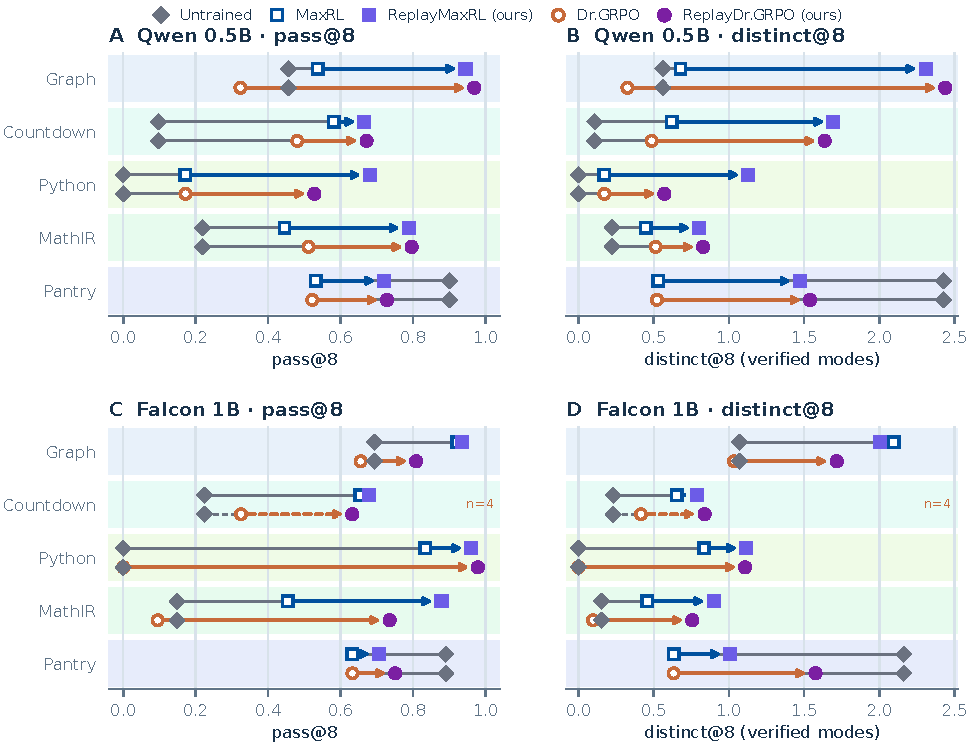
\includegraphics[width=.98\linewidth]
    {figures/e118_scale_extensions_appendix.pdf}
  \caption{\textbf{Per-domain results behind the cross-domain averages in
  Figure~\ref{fig:maxrl-factorial}.} Panels A--B show Qwen2.5-0.5B and panels
  C--D show Falcon3-1B. MaxRL--ReplayMaxRL pairs retain five terminal seeds
  in every domain. Dr.GRPO--ReplayDr.GRPO uses four admissible seeds for
  Falcon Countdown and five elsewhere. Domain tints match
  Figure~\ref{fig:modebench-examples}.
  Replay arrows, trained-arm markers, and untrained references use the same
  encoding as the main figure.}
  \label{fig:maxrl-factorial-scale-extensions}
\end{figure}

All five Qwen2.5-0.5B ReplayMaxRL--MaxRL blocks are complete. Both endpoint
effects are positive in every domain: \texttt{pass@8} effects range from
\(+.084\) to \(+.509\), and raw \texttt{distinct@8} effects range from
\(+.356\) to \(+1.630\). All five Falcon MaxRL--ReplayMaxRL blocks are also complete. ReplayMaxRL has a
positive mean \texttt{pass@8} effect in every Falcon domain and a positive raw
\texttt{distinct@8} effect in four of five. Graph is the exception on raw
support, with \(-.093\) modes (unadjusted 95\% interval
\([-.229,+.043]\)) and a small correctness effect of \(+.014\)
(\([-.016,+.044]\)). MathIR has the largest Falcon effects: \(+.424\) on
\texttt{pass@8} (\([+.310,+.539]\)) and \(+.443\) on
\texttt{distinct@8} (\([+.317,+.569]\)). The within-seed cross-domain
effects are \(+.133\) (\([+.043,+.223]\)) and \(+.228\)
(\([+.094,+.361]\)), respectively. Falcon Python remains inconclusive despite
positive means: \(+.127\) (\([-.372,+.625]\)) and \(+.280\)
(\([-.209,+.769]\)).

\textbf{The completed Qwen2.5-3B Python block extends the breadth result.}
All five seeds, 70--74, now have valid pass-8 endpoints for all four arms
(Table~\ref{tab:qwen3b-python-factorial}). ReplayMaxRL raises raw
\texttt{distinct@8} relative to MaxRL by \(+.391\)
(unadjusted paired 95\% interval \([+.079,+.704]\)); every paired seed has a
positive raw-support effect. The mean correctness gain is \(+.277\), but its
interval \([-.037,+.590]\) includes zero. This supports a domain-specific
breadth benefit at the larger model, without establishing a correctness gain
or a model-size trend. The other four Qwen2.5-3B domains remain incomplete;
no Qwen2.5-3B cross-domain average is reported.

\begin{table}[H]
  \centering
  \caption{\textbf{Newly completed Qwen2.5-3B Python factorial.}
  Means use all five registered seeds, 70--74, at exactly pass 8.
  The paired ReplayMaxRL--MaxRL effects and their unadjusted intervals are
  reported in the text; arm means alone are not paired effects.}
  \label{tab:qwen3b-python-factorial}
  \small
  \begin{tabular}{@{}lrrr@{}}
    \toprule
    \textbf{Method} & \(n\) & \textbf{pass@8} & \textbf{distinct@8} \\
    \midrule
    \input{results/e118_qwen3b_python_terminal_table_body.tex}
    \bottomrule
  \end{tabular}
\end{table}

\subsection{Interpretation boundary}
\label{app:scale-boundary}

At terminal pass 8, the ReplayDr.GRPO contrast has 24 admissible Falcon3-1B
pairs and 25 Qwen2.5-3B pairs. Falcon Countdown uses four seeds; the other
blocks use five. Raw \texttt{distinct@8} is higher in every admissible pair. Correctness-adjusted
breadth is strongest on Graph coloring, Countdown, and PantryPlan; Python
factors and MathIR more often improve correctness without a consistent breadth effect. These are per-domain,
within-scale comparisons. They do not establish monotonic improvement with
parameter count. MaxRL--ReplayMaxRL pair results use their own admissible seed sets;
full factorial interactions use the four-arm intersection. Incomplete Level-2
blocks remain descriptive and do not support cross-domain generality.

\section{Reproducibility and Claim Boundaries}
\label{app:reproducibility}

\subsection{Comparison registry}
\label{app:program-registry}

\begin{table}[H]
  \centering
  \caption{\textbf{The three experiments and the evidence boundary at the
  September 4 freeze.} A complete block contains all five registered paired
  terminal seeds. Partial or source-excluded intersections are not counted as complete blocks.
  E120 uses its September 4, 15:40:26 UTC snapshot.}
  \label{tab:experiment-map}
  \scriptsize
  \setlength{\tabcolsep}{3pt}
  \begin{tabularx}{\linewidth}{@{}P{.09\linewidth}P{.27\linewidth}P{.25\linewidth}P{.15\linewidth}Y@{}}
    \toprule
    & \textbf{Question} & \textbf{Registered unit} & \textbf{Complete} &
      \textbf{Still needed} \\
    \midrule
    Exp. 1 & Does canonical replay retain verified support? &
      Level 1; 3 scales $\times$ 5 domains; Dr./ReplayDr. &
      14/15 blocks; one $n=4$ & retain Falcon Countdown as descriptive after source exclusion \\
    Exp. 2 & Does memory add value beyond MaxRL? &
      Level 1; 3 scales $\times$ 5 domains; MaxRL/ReplayMaxRL &
      11/15 blocks & four Qwen-3B blocks; full factorial has ten complete blocks and one $n=4$ \\
    Exp. 3 & Does the factorial transfer to a harder matched level? &
      Level 2; Qwen-0.5B; 5 domains $\times$ 4 methods &
      1/5 blocks; Graph complete; MathIR \(n=1\) & finish the other four domains \\
    Ablation & Does fresh-frequency replay differ from uniform key replay? &
      Level 1; 9 model--domain blocks; 45 cells &
      5/9 blocks; 25/45 cells & larger-model blocks absent from the frozen E120 snapshot \\
    \bottomrule
  \end{tabularx}
\end{table}


The primary registry is the $2\times2$ factorial over fresh objective
(Dr.GRPO or MaxRL) and verified replay (off or on). Level 1 covers five domains
at Qwen2.5-0.5B, Falcon3-1B, and Qwen2.5-3B; Level 2 repeats the full factorial
on a separately generated, support-matched set at Qwen2.5-0.5B. A result enters
the paper only at a registered checkpoint shared by the paired methods. Seed
prefixes are labeled with exact $n$ and are never promoted to five-seed
estimates. GRPO, UCPO, sparse RLEP-Dr, and fixed Semantic MaxEnt remain direct
comparators rather than components of the primary factorial. The eleven complete
MaxRL--ReplayMaxRL blocks remain valid at five seeds each. Requiring all four
arms leaves ten complete five-seed blocks and one four-seed Falcon Countdown
block. Cross-objective interactions require the common admissible seed
intersection; they are not differences of aggregates with different seed sets.

\subsection{Training and evaluation contract}
\label{app:repro-run-contract}

\begin{table}[H]
  \centering
  \caption{\textbf{Core matched run contract.} Scale-specific systems changes
  are applied to every method within a paired comparison, so systems changes
  cannot define a treatment arm.}
  \label{tab:run-contract}
  \small
  \begin{tabularx}{\linewidth}{@{}P{.24\linewidth}Y@{}}
    \toprule
    \textbf{Component} & \textbf{Frozen setting} \\
    \midrule
    Data & 384 training and 128 disjoint evaluation prompts per domain and
      level; no evaluation row enters training or replay. \\
    Rollouts & $G=16$, temperature 1, top-$p=1$; one prompt group per update. \\
    Training & Eight passes (3,072 updates), one PPO epoch,
      $\beta_{\mathrm{KL}}=0$; paired methods share initialization, prompt stream,
      optimizer, and checkpoint cadence. \\
    Evaluation & Passes $0,.5,\ldots,8$; a separate temperature-0 greedy
      trace and four fixed temperature-1, top-$p=1$, $K=8$ draws per prompt for
      \texttt{pass@8}, \texttt{mean@8}, and \texttt{distinct@8}; no
      best-checkpoint selection. \\
    Replay & One capacity-16 bank per prompt; one bank selected by a serialized
      round-robin cursor per update; $\lambda_{\mathrm{replay}}=.10$; controls
      use the same replay code with an exact-zero derivative; realized banks and workloads can differ. \\
    \bottomrule
  \end{tabularx}
\end{table}

The pinned revisions are listed separately to keep model identity explicit:
\begin{itemize}
  \item Qwen2.5-0.5B-Instruct: {\scriptsize\texttt{7ae557604adf67be50417f59c2c2f167def9a775}};
  \item Falcon3-1B-Instruct: {\scriptsize\texttt{28ba2251970a01dd1edc7ba7dad2eb71216ccfdf}};
  \item Qwen2.5-3B-Instruct: {\scriptsize\texttt{aa8e72537993ba99e69dfaafa59ed015b17504d1}}.
\end{itemize}
Training seeds are 43--47, 55--59, and 70--74, respectively. Qwen2.5-0.5B uses a constant
$2\times10^{-7}$ learning rate; Falcon3-1B uses the same rate with optimizer
state offload; Qwen2.5-3B uses a $10^{-7}$ peak cosine schedule, $10^{-8}$
floor, and 10\% warmup. Every paired comparison uses the same hardware class
within its model--domain--seed block.

Graph coloring and Countdown allow 192 response tokens; Python factors uses
192/512/192 tokens at 0.5B/1B/3B; MathIR uses 64/128/64; PantryPlan uses eight.
Evaluation base seeds are 610100, 610200, 610300, 610400, and 76299 in domain
order. Sampled draw $d$ uses base seed plus $d$, with independent responses
within each draw. Metrics average over all 128 prompts and four draws; raw
prompt responses, per-draw endpoints, and their aggregate spread are retained.
Evaluation outputs never enter training, replay, checkpoint choice, or stopping.

\subsection{Recovery and fail-closed rules}
\label{app:repro-recovery}

Model and optimizer state, bank contents, replay cursor, data cursor, and random
request-stream state are checkpointed atomically. Resume checks schema,
capacity, scheduler settings, objective constants, token types, prompt hashes,
exemplar/key consistency, and cursor bounds. Non-finite values, state mismatch,
missing completion markers, changed data identities, or aggregate drift are
hard failures. Placement-only recovery amendments may change hardware or wall
time but not the scientific update.

\subsection{Artifacts and implementation map}
\label{app:repro-artifacts}
\label{app:repro-code}

Every reported figure has an adjacent machine-readable record containing its
source paths, exact seed set, checkpoint rule, displayed values, and SHA-256
hashes. \path{paper/FIGURE_MANIFEST.md} maps figures to builders and versioned
records. The ModeBench example renderer re-executes every displayed coloring,
factorization, arithmetic transition, and pantry allocation. Result builders
abort on missing matched comparisons or source-hash drift rather than carrying a
shallower checkpoint forward.

Under \path{src/oat_drgrpo/}, benchmark environments are implemented in
\path{canonical_actions.py}, \path{python_modebench.py}, \path{mathir.py}, and
\path{pantry_plan.py}; isolated Python execution uses
\path{python_modebench_process.py} and \path{python_modebench_worker.py}.
Verified replay and bank state are implemented in
\path{canonical_replay.py} and \path{online_canonical_bank.py}; learner
integration is in \path{learner/grpo.py} and \path{learner/run.py}. The
post-hoc raw-collapse and token-entropy audit is regenerated by
\path{ops/exp_scaling/build_paper_e78_python_collapse_diagnostics.py} into
\path{paper/results/e78_python_collapse_diagnostics.json}. E119 all-domain
terminal progress is stored beside Figure~\ref{fig:level2-admission}; E120-R1 is
regenerated by \path{ops/exp_scaling/build_paper_e120_frequency_progress.py}
into \path{paper/results/e120_frequency_progress.json} and its table body.
Dataset manifests under \path{var/data/} bind every train/evaluation identity
and level.

\section{Limitations and Disclosures}
\label{app:limitations}

Appendix~\ref{app:theory} gives categorical collapse and retention
results, plus conditional extensions to stochastic updates and bank admission.
These require the stated geometry, energy, and coverage assumptions; they do
not certify the implemented neural optimizer. Convergence to uniform correct
mass in the categorical uniform-replay model requires full verified coverage,
which Python's bank capacity precludes. ModeBench measures
task-defined executable support on small synthetic tasks rather than free-form
reasoning diversity or downstream utility. Experiments fix \(G=16\), zero
reference KL, no token-entropy bonus, and a single decoding protocol; dynamic
sampling, larger groups, regularization, and decoding sweeps remain open. The
uniform-versus-frequency ablation has five of nine complete blocks, all at
Qwen2.5-0.5B, in the frozen September 4, 15:40:26 UTC E120 snapshot. The across-scale
MaxRL pair has 11/15 complete blocks; requiring all four arms leaves ten
complete blocks and one four-seed block. Core replay evidence contains 14
complete blocks and one four-seed block. Level-2 transfer remains complete
only on Graph. Sign tests are nominal exploratory summaries assuming
independent block signs; individual intervals quantify estimation uncertainty.

\subsection{AI Use Statement}
\label{sec:ai-use}

In this work, we used a general-purpose generative AI tool to organize and
copy-edit the manuscript, help interpret recorded experimental results for
reporting, develop and check mathematical arguments, write auxiliary
result-reporting code, and check internal consistency, sources, formatting,
and compilation. We did not use the tool to
generate experimental observations, select reported checkpoints, alter
registered stopping rules, or make final decisions about scientific claims.
Every numerical statement is regenerated from the recorded run artifacts by
the scripts identified in Appendix~\ref{app:reproducibility}. The authors
reviewed all AI-assisted prose, code, and claims and take responsibility for the
final content of this work.

\subsection{Ethics Statement}

The benchmark and experiment-specific data are synthetic; this study collects
no human-subject or personal data. More verified modes are not inherently
better: a distinct execution may be risky or costly even when it passes the
validator, and \texttt{distinct@}$K$ does not measure downstream value. Systems
that evaluate or optimize breadth should report correctness, invalidity, and
application-specific costs alongside mode counts.

\subsection{Reproducibility Statement}

Claims are computed from versioned result files; missing final results and aggregate drift cause the build to
fail. Appendix~\ref{app:reproducibility} records protocols, hashes, validations,
and regeneration commands; Appendix~\ref{app:data} records split identities.
The AI Use Statement above discloses generative-AI assistance.



\end{document}
